%%%%%% IMPORTAÇÃO DOS PACOTES %%%%%%
\documentclass[
	% -- opções da classe memoir --
	12pt,				% tamanho da fonte
	openright,			% capítulos começam em páginas ímpar (insere página vazia caso preciso)
	oneside,			% para impressão em verso e anverso. Oposto a oneside
	a4paper,		% tamanho do papel.
	% -- opções da classe abntex2 --
	chapter=TITLE,		% títulos de capítulos convertidos em letras maiúsculas
	section=TITLE,		% títulos de seções convertidos em letras maiúsculas
	%subsection=TITLE,	% títulos de subseções convertidos em letras maiúsculas
	%subsubsection=TITLE,% títulos de subsubseções convertidos em letras maiúsculas
	% -- opções do pacote babel --
    brazil,				% o último idioma é o principal do documento
	english,			% idioma adicional para hifenização
	%french,			% idioma adicional para hifenização
	%spanish,			% idioma adicional para hifenização
	sumario=tradicional,
	]{abntex2}

% --------------- PACOTES -----------------%
%%%%% conflict with float package, loaded by one of the packages bellow.
% \usepackage{floatrow} % pacote para criar ambientes float genéricos
% \floatsetup[table]{style=plaintop} % poe legendas de tabelas em cima.

% Pacotes fundamentais
\usepackage{cmap}				% Mapear caracteres especiais no PDF
\usepackage{lmodern}			% Usa a fonte Latin Modern
\usepackage[T1]{fontenc}		% Selecão de códigos de fonte. hifenação correta.
\usepackage[utf8]{inputenc}		% Codificacao do documento (conversão automática dos acentos)
\usepackage{lastpage}			% Usado pela Ficha catalográfica
\usepackage{indentfirst}		% Indenta o primeiro parágrafo de cada seção.
\usepackage{xcolor}				% Controle das cores
\usepackage[pdftex]{graphicx}	% Inclusão de gráficos
\graphicspath{{figures/}}
\usepackage{subcaption}
\usepackage{epstopdf}           % Pacote que converte as figuras em eps para pdf


% Pacotes adicionais, usados apenas no âmbito do Modelo Canônico do abnteX2
\usepackage{nomencl}
\usepackage{amsmath}   % usado para ter o environment pmatrix, align
\usepackage{mathtools} % usado para ter o environment pmatrix*
\usepackage{mathrsfs}  % usado para ter o curly H
\usepackage{xfrac}     % usado para ter o comando \sfrac
\usepackage{bbm}
\usepackage[chapter]{algorithm}
\usepackage{algorithmic}
\usepackage{multirow}
\usepackage{rotating}
\usepackage{pdfpages}       % insere páginas pdf no arquivo
\usepackage{siunitx}        % pacote para padronizar display de números e unidades

\usepackage[brazilian,hyperpageref]{backref}	 % Paginas com as citacões na bibl

\usepackage[toc,acronym,nomain,nogroupskip,nonumberlist]{glossaries}%nonumberlist
\newacronym{linac}{LINAC}{Linear Accelerator}
\newacronym{cnpem}{CNPEM}{National Center for Research in Energy and Materials}
\newacronym{lnls}{LNLS}{Brazilian Synchrotron Light Laboratory}
\newacronym{3gls}{3$^\text{rd}$ GLS}{Third Generation Light Sources}
\newacronym{4gls}{4$^\text{th}$ GLS}{Fourth Generation Light Sources}
\newacronym{mac}{MAC}{Machine Advisory Committee}
\newacronym{bsc}{BSC}{Beam Stay Clear}
\newacronym{supcond}{SC-RF}{Superconducting RF Cavity}
\newacronym{csr}{CSR}{coherent synchrotron radiation}
\newacronym{dsp}{DSP}{direct space charge}
\newacronym{isp}{ISP}{indirect space charge}
\newacronym{maxeq}{ME}{Maxwell Equations}
\newacronym{lhs}{l.h.s.}{left hand side}
\newacronym{rhs}{r.h.s.}{right hand side}
\newacronym{xfel}{FEL}{X-Ray Free Electron Lasers}
\newacronym{als}{ALS}{Advanced Light Source}
\newacronym{cern}{CERN}{European Organization for Nuclear Research}
\newacronym{neg}{NEG}{Non--Evaporable Getter}
\newacronym{pec}{PEC}{Perfect Electric Conductor}
\newacronym{esrf}{ESRF}{European Synchrotron Radiation Facility}
\newacronym{mba}{MBA}{Multi-Bend-Achromat}
\newacronym{tmci}{TMCI}{Transverse Mode-Coupling Instability}
\newacronym{lmci}{LMCI}{Longitudinal Mode-Coupling Instability}
\newacronym{fofb}{FOFB}{Fast Orbit Feedback System}
\newacronym{apu}{APU}{Adjustable Phase Undulator}
\newacronym{rms}{rms}{root-mean-square}
\newacronym{vfp}{VFP}{Vlasov Fokker Planck}
\newacronym{si}{SI}{International System of Units}
\newacronym{ibs}{IBS}{intrabeam scattering}
\newacronym{pic}{PIC}{particle in cell}
\newacronym{dc}{DC}{direct current}

\newglossaryentry{bpm}
{
  name={BPM},
  description={Beam Position Monitor},
  first={\glsentrydesc{bpm} (\glsentrytext{bpm})},
  plural={BPMs},
  descriptionplural={Beam Position Monitors},
  firstplural={\glsentrydescplural{bpm} (\glsentryplural{bpm})}
}
\newglossaryentry{sls}
{
  name={SLS},
  description={Synchrotron Light Source},
  first={\glsentrydesc{sls} (\glsentrytext{sls})},
  plural={SLSs},
  descriptionplural={Synchrotron Light Sources},
  firstplural={\glsentrydescplural{sls} (\glsentryplural{sls})}
}
\newglossaryentry{id}
{
  name={ID},
  description={Insertion Device},
  first={\glsentrydesc{id} (\glsentrytext{id})},
  plural={IDs},
  descriptionplural={Insertion Devices},
  firstplural={\glsentrydescplural{id} (\glsentryplural{id})}
}
\newglossaryentry{bbr}
{
  name={BBR},
  description={broad band resonator},
  first={\glsentrydesc{bbr} (\glsentrytext{bbr})},
  plural={BBRs},
  descriptionplural={broad band resonators},
  firstplural={\glsentrydescplural{bbr} (\glsentryplural{bbr})}
}
\newglossaryentry{hom}
{
  name={HOM},
  description={higher order mode},
  first={\glsentrydesc{hom} (\glsentrytext{hom})},
  plural={HOMs},
  descriptionplural={higher order modes},
  firstplural={\glsentrydescplural{hom} (\glsentryplural{hom})}
}


% Pacote que faz Citações padrão ABNT
\usepackage[
alf,
versalete,
abnt-and-type=&,
abnt-etal-cite=2,
abnt-etal-list=3,
abnt-doi=link,
% abnt-repeated-author-omit=yes,
abnt-etal-text=emph]{abntex2cite}
% \citebrackets[]
% \usepackage[style=numeric-comp]{biblatex}
\renewcommand{\authorcapstyle}{\small}
\renewcommand{\authorstyle}{\relax}

% Pacote de customização - Unicamp
\usepackage{unicamp}

% Pacote para fazer desenhos
\usepackage{tikz}
%\usetikzlibrary{⟨list of libraries separated by commas⟩} % carrega bibliotecas adicionais
\usetikzlibrary{calc,arrows.meta}


% Pacotes de Debbuging:
\usepackage{lipsum}     % Pacote que gera texto dummy
%\usepackage{blindtext}  % Pacote que gera texto dummy
% \usepackage{showlabels} % Pacote que mostra os labels das equações no pdf
\usepackage{todonotes}  % Pacote que insere notas no pdf

% Posso criar definições de acrônimos e ele automaticamente coloca o nome completo
% no texto na primeira ocorrência ou o acrônimo nas referências subsequentes
% \frenchspacing
% \renewcommand{\finalnamedelim}{\ \&\ }
% \makenoidxglossaries
% \newacronym{linac}{LINAC}{Linear Accelerator}
\newacronym{cnpem}{CNPEM}{National Center for Research in Energy and Materials}
\newacronym{lnls}{LNLS}{Brazilian Synchrotron Light Laboratory}
\newacronym{3gls}{3$^\text{rd}$ GLS}{Third Generation Light Sources}
\newacronym{4gls}{4$^\text{th}$ GLS}{Fourth Generation Light Sources}
\newacronym{mac}{MAC}{Machine Advisory Committee}
\newacronym{bsc}{BSC}{Beam Stay Clear}
\newacronym{supcond}{SC-RF}{Superconducting RF Cavity}
\newacronym{csr}{CSR}{coherent synchrotron radiation}
\newacronym{dsp}{DSP}{direct space charge}
\newacronym{isp}{ISP}{indirect space charge}
\newacronym{maxeq}{ME}{Maxwell Equations}
\newacronym{lhs}{l.h.s.}{left hand side}
\newacronym{rhs}{r.h.s.}{right hand side}
\newacronym{xfel}{FEL}{X-Ray Free Electron Lasers}
\newacronym{als}{ALS}{Advanced Light Source}
\newacronym{cern}{CERN}{European Organization for Nuclear Research}
\newacronym{neg}{NEG}{Non--Evaporable Getter}
\newacronym{pec}{PEC}{Perfect Electric Conductor}
\newacronym{esrf}{ESRF}{European Synchrotron Radiation Facility}
\newacronym{mba}{MBA}{Multi-Bend-Achromat}
\newacronym{tmci}{TMCI}{Transverse Mode-Coupling Instability}
\newacronym{lmci}{LMCI}{Longitudinal Mode-Coupling Instability}
\newacronym{fofb}{FOFB}{Fast Orbit Feedback System}
\newacronym{apu}{APU}{Adjustable Phase Undulator}
\newacronym{rms}{rms}{root-mean-square}
\newacronym{vfp}{VFP}{Vlasov Fokker Planck}
\newacronym{si}{SI}{International System of Units}
\newacronym{ibs}{IBS}{intrabeam scattering}
\newacronym{pic}{PIC}{particle in cell}
\newacronym{dc}{DC}{direct current}

\newglossaryentry{bpm}
{
  name={BPM},
  description={Beam Position Monitor},
  first={\glsentrydesc{bpm} (\glsentrytext{bpm})},
  plural={BPMs},
  descriptionplural={Beam Position Monitors},
  firstplural={\glsentrydescplural{bpm} (\glsentryplural{bpm})}
}
\newglossaryentry{sls}
{
  name={SLS},
  description={Synchrotron Light Source},
  first={\glsentrydesc{sls} (\glsentrytext{sls})},
  plural={SLSs},
  descriptionplural={Synchrotron Light Sources},
  firstplural={\glsentrydescplural{sls} (\glsentryplural{sls})}
}
\newglossaryentry{id}
{
  name={ID},
  description={Insertion Device},
  first={\glsentrydesc{id} (\glsentrytext{id})},
  plural={IDs},
  descriptionplural={Insertion Devices},
  firstplural={\glsentrydescplural{id} (\glsentryplural{id})}
}
\newglossaryentry{bbr}
{
  name={BBR},
  description={broad band resonator},
  first={\glsentrydesc{bbr} (\glsentrytext{bbr})},
  plural={BBRs},
  descriptionplural={broad band resonators},
  firstplural={\glsentrydescplural{bbr} (\glsentryplural{bbr})}
}
\newglossaryentry{hom}
{
  name={HOM},
  description={higher order mode},
  first={\glsentrydesc{hom} (\glsentrytext{hom})},
  plural={HOMs},
  descriptionplural={higher order modes},
  firstplural={\glsentrydescplural{hom} (\glsentryplural{hom})}
}

% comando \gls


%---------------CONFIGURAÇÕES------------%

% informações do PDF. O pacote hyperref já foi incluido em abntex2, eu acho
\makeatletter
\hypersetup{
     	%pagebackref=true,
		pdftitle={\@title},
		pdfauthor={\@author},
    	pdfsubject={\imprimirpreambulo},
	    pdfcreator={LaTeX with abnTeX2},
		pdfkeywords={abnt}{latex}{abntex}{abntex2}{trabalho acadêmico},
		hidelinks,					% desabilita as bordas dos links
		colorlinks=false,       	% false: boxed links; true: colored links
    	linkcolor=blue,          	% color of internal links
    	citecolor=blue,        		% color of links to bibliography
    	filecolor=magenta,      	% color of file links
		urlcolor=blue,
%		linkbordercolor={1 1 1},	% set to white
		bookmarksdepth=4
}
\makeatother

% Espaçamentos entre linhas e parágrafos
\setlength{\parindent}{1.3cm} % Tamanho da identação do parágrafo
% Controle do espaçamento entre um parágrafo e outro:
\setlength{\parskip}{0.2cm}  % tente também \onelineskip

%\setlength{\mathindent}{0cm}

% Compila o índice
\makeindex
\makenomenclature

% \bibliography{library}

% Informacoes de dados para CAPA e FOLHA DE ROSTO:
\titulo{Estudo de Impedâncias e Instabilidades Coletivas aplicadas ao Sirius.}
\autor{Fernando Henrique de Sá}
\local{Campinas}
\data{2017}
\orientador[Orientador:]{Prof. Dr. Antônio Rubens Britto de Castro}
\coorientador[Co-orientador:]{Prof. Dr. Silvio Antonio Sachetto Vitiello}
\instituicao{%
    UNIVERSIDADE ESTADUAL DE CAMPINAS
    \par
    Instituto de Física Gleb Wataghin (IFGW)
    }
\tipotrabalho{Tese (Doutorado)}
% O preambulo deve conter o tipo do trabalho, o objetivo, o nome da instituição
% e a área de concentração
\preambulo{Tese apresentada ao Instituto de Física Gleb Wataghin (IFGW) da
           Universidade Estadual de Campinas (UNICAMP) como parte dos
           requisitos exigidos para a obtenção do título de Doutor em Física,
           com ênfase em Física de Aceleradores.}

\newcommand{\udefint}[2]{\int\!\!\text{d}#1 #2}                 % Integral indefinida
\newcommand{\udefoint}[2]{\oint\!\text{d}#1 #2}               % Integral fechada
\newcommand{\defint}[4]{\int_{#3}^{#4}\!\!\text{d}#1 #2}       % Integral definida
\newcommand{\infint}[2]{\defint{#1}{#2}{-\infty}{\infty}}      % Integra definida infinito
\newcommand{\dertot}[3][{}]{\frac{\mathrm{d}^{#1}#2}{\mathrm{d} #3^{#1}}} % Derivada total
\newcommand{\derpar}[3][{}]{\frac{\partial^{#1}#2}{\partial #3^{#1}}}     % Derivada parcial
\newcommand{\average}[2][{}]{\left\langle #2 \right\rangle_{#1}}
\newcommand{\vect}[1]{\overrightarrow{\boldsymbol{#1}}}
\newcommand{\versor}[1]{\boldsymbol{\hat#1}}
\newcommand{\tensor}[1]{\overleftrightarrow{\boldsymbol{#1}}} % Tensor
\newcommand{\fourier}[1]{\tilde{#1}}  % representation of the Fourier Transform
\newcommand{\real}[1]{\Re\left\{#1\right\}}
\newcommand{\imag}[1]{\Im\left\{#1\right\}}
\newcommand{\engw}[1]{\emph{#1}}        % Palavra em Língua Inglesa


% \includeonly{
% % %content/Chap1-introducao,
% % content/Chap2-fisica_aceleradores,
% % content/Chap3-impedancias_e_wakes,
% % %content/App1-derivacoes,
% }

\begin{document}
	% Retira espaço extra obsoleto entre as frases
	\frenchspacing

	%---------- Elementos pré-textuais --------------%
	\pretextual
	%Capa
\imprimircapa


%Folha de rosto sem número de página
\setcounter{page}{3}
\imprimirfolhaderosto*


% Ficha Catalográfica
% Não sei o que é ainda, mas parece que a universidade vai me fornecer uma
%após a defesa da minha tese. Quando ela fizer isso, tenho que comentar as
%linhas abaixo e descomentar o \includepdf:
\begin{fichacatalografica}
    \vspace*{\fill}
    \begin{center}
        \textsc{Inclua aqui o pdf com a ficha catalográfica fornecida pela BAE.}
    \end{center}
    \vspace*{\fill}
    %\includepdf{ficha-catalografica.pdf}
\end{fichacatalografica}


% Folha de aprovação
% Na versão final, tenho que excluir essas linhas e incluir o \includepdf
\newpage
\vspace*{\fill}
\begin{center}
    \textsc{Inclua aqui a folha de assinaturas.}
\end{center}
\vspace*{\fill}
\newpage
%\includepdf[pagecommand={\thispagestyle{plain}}]{folha-assinaturas.pdf}
\cleardoublepage


% Dedicatória
\begin{dedicatoria}
    \vspace*{\fill}
    \centering
    \noindent
    \textit{Dedico esta tese à todo mundo.}
    \vspace*{\fill}
\end{dedicatoria}

% Agradecimentos
\begin{agradecimentos}
    \lipsum[1-4]
\end{agradecimentos}

% Epígrafe
\begin{epigrafe}
    \vspace*{\fill}
    \begin{flushright}
        \textit{``Aqui jaz seis anos da minha vida.''\\
        (Fernando Henrique de Sá)}
    \end{flushright}
\end{epigrafe}

% Resumos em português
\begin{resumo}
    \lipsum[1-2]
    \vspace{\onelineskip}
    \noindent\textbf{Keywords}: keyword 1; keyword 2; keyword 3.
    \vspace{\fill}
\end{resumo}

% Resumo em Inglês
\begin{otherlanguage*}{brazil}
    \begin{center}{\ABNTEXchapterfont\huge Resumo}\end{center}

    \lipsum[1-2]
    \vspace{\onelineskip}
    \noindent\textbf{Palavras-chaves}: palavra-chave 1; palavra-chave 2; palavra-chave 3.
    \vspace{\fill}
\end{otherlanguage*}
\cleardoublepage


% Lista de ilustrações
\pdfbookmark[0]{\listfigurename}{lof}
\listoffigures*
\cleardoublepage


% Lista de tabelas
\pdfbookmark[0]{\listtablename}{lot}
\listoftables*
\cleardoublepage


% Lista de Acronimos e Abreviações
\renewcommand{\nomname}{Lista de Acrônimos e Abreviações}
\pdfbookmark[0]{\nomname}{las}
\printnomenclature
\cleardoublepage


% Sumário
\pdfbookmark[0]{\contentsname}{toc}
\tableofcontents*
\cleardoublepage


	%---------- Elementos textuais ------------------%
	\textual

%%%%%%%%%%%%%%%%%%%%%%%%%%%%%%%%%%%%%%%%%%%%%%%%%%%%%%%%%%%%%%%%%%%%%
%%%%%%%%%%%%%%%%%%%%%%%%%%%%%%%%%%%%%%%%%%%%%%%%%%%%%%%%%%%%%%%%%%%%%
\chapter{Introduction} \label{chap:intro}

	In scientific facilities commonly known as \gls{sls} the interaction between light and matter is used to study properties of a variaty of materials. Through techniques envolving absortion, reflection, refraction and scattering of light of different 'colors' by the materials under study, their atomic structure, composition and chemical activity can be determined.

  	The frequency of the light used in these facilities ranges from tera-hertz to hard X-rays and its origin is always related to synchrotron emission of radiation by charged particles, hence the name of the facility. The light emitted by centripetal acceleration of ultra-relativistic particles has unique properties for use in scientific investigation: broad spectrum, high total flux and the strong collimation are among them.

\section{Types of Light Sources}

    In general we can separate the \gls{sls} in two groups, depending on the topology of the accelerators involved: linear and circular. In the linear sources, denominated \gls{fel}, it is possible to excite the beam to emit light coherently, hence the name of these facilities. There are several techniques to achieve this and their enumeration or explanation is beyond the scope of this work~\cite{saseref,other_methods}. The important fact is that besides the high level of coherence of the light in these facilities, the intensity of the photon beam is increased by orders of magnitude with these techniques because it becomes proportional to the square of the number of particles in the beam, instead of the linear dependency of other sources. The excitation of coherent emission becomes increasingly difficult as the energy of the photons increase, because ever smaller errors in the fields or decoherences in the electron beam destroy the cascade of the stimulated emission. This task is so difficult that only in the last decade coherent X-rays were successfully generated by new machines that were built specially for that, the X-\gls{fel}. This achievement represented a revolution in the synchrotron radiation community and opened up exciting new possibilities for scientific research~\cite{some,scientific,papers}.

    Among the several types of circular accelerators we highlight the ones based on synchrotron storage rings. There is an abuse of use of the word synchrotron here, so far it meant the nature of emission of the light in these facilities, but when used to describe this type of accelerator it is related to the synchronicity of the revolution time of the electrons with the electromagnetic field that drives their motion, which is the main mechanism behind the operation of these machines. In this type of \gls{sls} the electrons are grouped in several bunches that fill the whole storage ring and are confined for hours in close to circular orbits by deflecting and focusing magnetostatic fields. The radiation used in experiments can be generated by the same fields that deflect the beam (dipoles) or by special devices called \gls{ids} that are put in empty sections of the ring, called straight sections.

    While the experiments in X-\gls{fel} are performed with only one strong single pulse of radiation that can be generated at a repetition rate of a few hundreads of Hertz, in storage rings the emitted light continuously hit the samples under study and the interaction patterns are recorded for as long as needed to achieve the desired resolution for the experiment. Besides, while in X-\gls{fel} it is only possible to have one beamline operating, in storage rings dozens of them can work simultaneously, performing completely different experiments.

    Figure~\ref{fig:light_source_example} shows a generic example of a storage ring based light source. It has three main subsystems: an injector, the storage ring and the beamlines. The injector is the responsible of generating and accelerating the particles up to the energy of the storage ring and in most light sources it is composed of a gun, a \gls{linac} and a booster synchrotron. In the case of electron storage rings the gun extract the electrons from metals, via thermoionic or photoelectric effect, and guide them to the \gls{linac} where they are compressed in bunches and accelerated, generally up to energies of hundreads of \si{\mega\electronvolt}. After this, the electrons are transported to the booster synchrotron where they are accelerated up to the energy of the storage ring, generally a few \si{\giga\electronvolt}, and extracted from it to be injected in the storage ring. In modern light sources this whole process can happen with a repetition rate of a few \si{\hertz}.

    \begin{figure}[b!]
        \center
        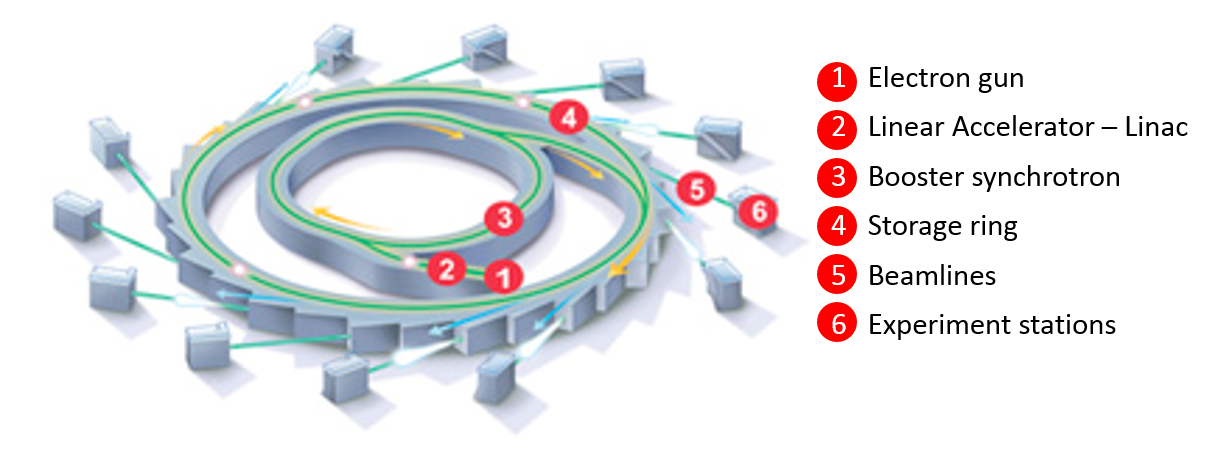
\includegraphics[width=\textwidth]{storage_ring_example.png}
        \caption[Schematic of a storage ring based light source.]{Schematic of a storage ring based light source. Notice the three main systems: the injection systems, composed of an electron gun, a \gls{linac} and a booster; the storage ring and the beamlines, with the experiment stations at their end.}
        \label{fig:light_source_example}
    \end{figure}

    The storage ring is a synchrotron just like the booster that, instead of accelerating the electrons, keeps their average energy fixed while they perform dozens of billions of turns in the few hours they remain there. After the injection, the bunch of electrons oscillate around the ideal orbit of the storage ring, but in a few dozens of thousands of turns they are damped, reaching the storage ring equilibrium values of transverse emittances (size and divergence), longitudinal length and energy spread. In ideal storage rings they stay stable in stationary closed orbits emitting radiation that is collected by the beamlines. The radiation exits the storage ring through holes in the external part of the vacuum chamber and propagate through the beamline in straight trajectories, tangent to the electrons orbit in the point where it was generated. Among all the elements in the beamlines, we highlight the monochromators, used to select a narrow energy bandwidth of the radiation, and the mirrors, which deflect and focus the photon beam to the samples, located at the end of the beamline, together with a complex apparatus to support it and measure its interaction data.

\section{Storage Ring Main Devices} \label{sec:storage_ring_main_devices}

    This work will focus on the study of the dynamics of the particles while they are in their equilibrium regime inside the storage ring, without considering the details of the injection process. For this reason, in this subsection we will present the main subsystems of a storage ring and discuss on their main contributions to the task of keeping particles confined for such long times.

\subsection{Magnetic Lattice}

    The magnetic lattice is the name of the series of static magnets that are placed along the beam trajectory that deflect and focus it to keep it circulating the ring. It is composed of a reduced number of different types of magnets that have specific functions for the beam confinement:
    \begin{description}[align=left]
        \item[Dipoles:] or bending magnets are the devices responsible for deflecting the beam in such a way that its liquid deflection in one turn is \SI{2\pi}{\radian}. They generate an almost constant vertical field, $B_y$, along the beam path that curves its horizontal trajectory and keeps the vertical unchanged, see Figure~\ref{fig:dipole}. At each point of the trajectory inside a dipole the curvature, $G(s)$, is given by:
        \begin{align}\label{eq:curvature_dipole}
            G(s) = \frac{1}{\rho(s)} = \frac{e}{p_0}B_y(s) \approx \frac{ec}{E_0}B_y(s)
        \end{align}
        \begin{figure}[t!]
            \center
            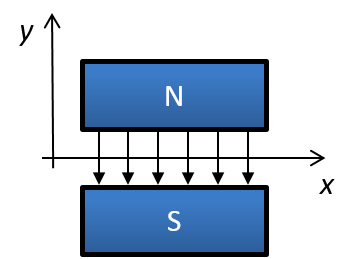
\includegraphics[width=0.4\textwidth]{dipole_example.png}
            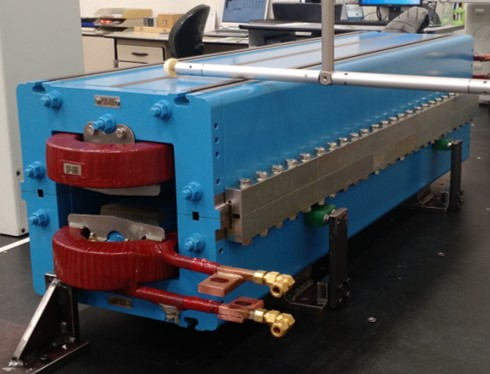
\includegraphics[width=0.5\textwidth]{dipole_real.jpg}
            \caption[Example of dipole magnet.]{Left: Schematic figure of a dipole magnet, where N and S indicate the North and South poles of the magnet and the vertical down arrows indicate the magnetic field lines. Right: Picture of a real dipole magnet.}
            \label{fig:dipole}
        \end{figure}
        where $s$ is the longitudinal position along the ring, $\rho(s)$ is the radius of curvature, $e$ is the absolute value of the particle's charge, $c$ is the speed of light, $p_0$ is the absolute value of the average linear momentum of the beam and $E_0$ is the average beam energy. Notice in the equation above that dipoles work as spectrometers, if the beam has an energy spread, particles with higher/lower energy will spiral out/in because their total deflection angle will be different than \SI{2\pi}{\radian}, which means eventually all particles will hit the vacuum chamber and be lost;
        \item[Quadrupoles:] are responsible to focus the beam, keeping the particles that are not in the ideal orbit oscillating around it. They achieve this by creating a field that grows linearly in intensity with the displacement from its center (see Figure~\ref{fig:quadrupole}), in such a way that they work as lenses. They are characterized by their strength, defined by:
        \begin{align}
            K(s) = \frac{e}{p_0}\left.\derpar{B_y}{x}\right|_{y=0}(s)
        \end{align}
        \begin{figure}[t!]
            \center
            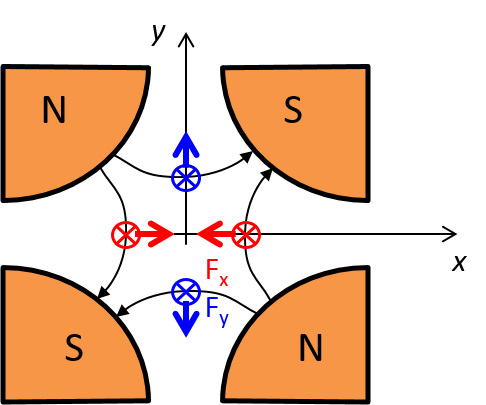
\includegraphics[width=0.4\textwidth]{quadrupole_example.png}
            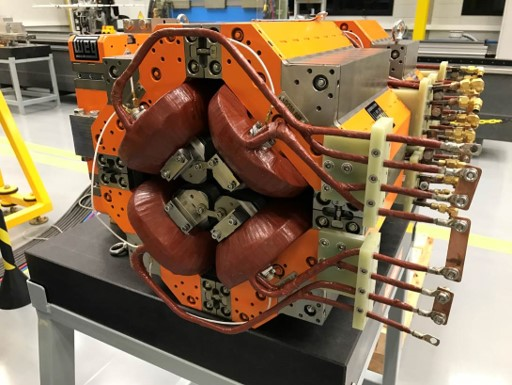
\includegraphics[width=0.5\textwidth]{quadrupole_real.jpg}
            \caption[Example of quadrupole magnet.]{Left: Schematic figure of a quadrupole magnet, where N and S indicate the North and South poles of the magnet, the curved arrows indicate the magnetic field lines and the red/blue arrows indicate the direction of the horizontal/vertical forces felt by an electron entering the sheet. Notice this quadrupole focuses in the horizontal, so it is a focusing quadrupole. Right: Picture of a real quadrupole magnet, with the coils that generate the magnetic field and the iron core that guide and shape the field lines inside the gap.}
            \label{fig:quadrupole}
        \end{figure}
        where $x$ is the horizontal displacement from the center of the quadrupole and $y$ is the vertical. The strength defined above is directly related to how much the quadrupole deflect off-centered particles, being its integral along the quadrupole length directly related to the focal distance of the magnet. One intrinsic limitation of quadrupoles imposed by \gls{maxeq} and the Lorentz force is that they cannot focus the beam simultaneously in the horizontal and vertical directions. This means that in a magnetic lattice it is always needed to have two types of quadrupoles, one to focus in the horizontal, called focusing quadrupoles, and one to focus in the vertical, called defocusing quadrupoles, in such a way that liquid focusing in both planes can be achieved with intelligent positioning of the magnets. Besides, quadrupoles are arranged along the ring to correct the intrinsic limitation of the dipoles regarding the energy dispersion, as discussed above, adding/subtracting liquid deflection in one turn for particles with more/less energy. This cause particles to have different closed orbits depending on their energy, but at least maintain them stable. Quadrupoles and dipoles are the most important multipoles in a storage ring because together they define its main properties, such as the particles average energy, the transverse beam emittance, and beam sizes along the ring, as well as the fundamental frequency of oscillation of the particles, the tune.
        \item[Sextupoles:] quadrupoles also suffer from chromatic aberrations, focusing more or less the particles depending on their energy. This difference in focusing makes particles oscillate differently around their closed orbit, changing their fundamental resonance frequency. This is not a fundamental problem, but in almost all modern storage rings it is impossible to store particles with only dipoles and quadrupoles. Sextupoles can correct that effect if placed at the right positions along the ring because of their non-linear magnetic field, which grows quadractically with the distance from its center, see Figure~\ref{fig:sextupole}. Just like quadrupoles, it is needed two types of sextupoles, focusing and defocusing, to correct the horizontal and vertical frequency of oscillation of the particles. Sextupoles are needed, but they introduce several complications for the design of a storage ring, because their non-linear fields introduce chaos in some regions of the particles phase space. More sextupoles or higher order multipoles can be introduced to avoid chaos as much as possible and also to help correcting higher order chromatic effects.
        \begin{figure}[t!]
            \center
            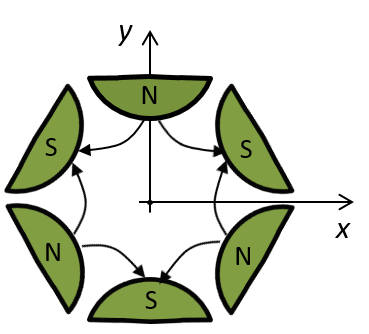
\includegraphics[width=0.4\textwidth]{sextupole_example.png}
            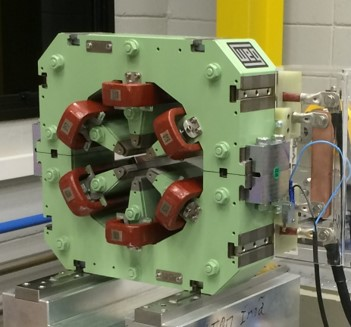
\includegraphics[width=0.5\textwidth]{sextupole_real.jpg}
            \caption[Example of sextupole magnet.]{Left: Schematic figure of a sextupole magnet, where N and S indicate the North and South poles of the magnet and the curved arrows indicate the magnetic field lines. Right: Picture of a real sextupole magnet.}
            \label{fig:sextupole}
        \end{figure}
    \end{description}

    Higher order multipoles, such as octupoles and decapoles, can be used to correct higher order chromatic and geometric aberrations, but their use is not very common in the design of storage ring for light sources as they are in colliders, even though this tendency is changing with the new light sources that are being designed~\cite{maxiv,esrfupgrade}. Nevertheless, they are always present in storage ring as errors of the main magnets and their effect must be taken into account in detailed single particle dynamics analysis.

    Generally lattices have high periodicity, being the repetition of a unit cell along the whole extension of the ring. This periodicity simplifies the design of the ring, the dynamics of the electrons and reduces the number of dangerous resonances that can harm the beam stability. Unit cells generally can be divided in two parts, an arc section, where are placed the dipoles, intervealed by focusing elements to control the dispersion and focus the beam from one dipole to another, and a straight section, with an empty space for the installation of \gls{ids} for light generation and some focusing elements to focus the beam in the center of these empty spaces.

\subsection{RF Cavity}

    Each turn the electrons lose energy due to synchrotron radiation which must be replenished periodically in order for them to remain in stable orbits, with energy close to the nominal energy of the storage ring. The magnetostatic components described above cannot perform such a task neither any other component or method relying on static electromagnetic fields of any kind, because according to the \gls{maxeq} and the Lorentz force, the liquid energy transfered to a charged particle by static fields in one turn over the ring must be zero. This means that the laws of physics constraint it is necessary to rely on time dependent electromagnetic fields to replenish the energy of the electrons. The way this is accomplished in a storage ring is through the use of devices called RF cavities.

    RF cavity is a jargon for a cylindrical electromagnetic cavity with the lowest Transverse Magnetic mode (TM010) in the range of radiofrequency. Cavities for use in storage rings must have at least two small holes in its axis for the beam passage and one other hole to couple the cavity with an external source to feed the mode TM010 with energy. This energy is transfered to the particles in the storage ring through the almost homogeneous longitudinal eletric field of this mode when the particles passes through the cavity. The frequency of this particular mode of the cavity is always exactly equal to a multiple, $h$, of the revolution frequency of the beam along the ring, in such a way that once initially adjusted, the beam will always enter the cavity when the electric field has a phase that replenish the average energy lost by it in one turn. Besides, this synchronicity mechanism, that, by the way, is the responsible for the name of these machines, creates $h$ points in the ring where it is possible to put a bunch of electrons around it and keep it stable.

\subsection{Vacuum System}

    The vacuum system is responsible for creating a compact region around the reference orbit in the whole machine with very low pressure, which minimize collisions of the stored charged particles with gas molecules and, consequently, increase the average time particles can be stored with stable movement. Quantitatively, the average pressure of a storage ring must be lower than \SI{1}{\nano Torr} for the average stored time of the particles to be of the order of a few dozens of hours.

    The vacuum system is composed of two main subsystems, the vacuum vessel, which defines the boundaries of the electrons atmosphere with the environment, and vacuum pumps to maintain the desired difference in pressure between the two regions. Most of the extension of the vacuum vessel is composed of straight and long chambers with a specific cross section, constant along the extension of the chamber. They are made of metals due to several desirable properties of these materials, such as high heat and electrical conductivity, maleability, high acceptance to yelding and brasing and high resistence to pressure. Among them we highlight implications of the high electrical conductivity, due to its importance for this work. Besides the standard vacuum chamber there are several other structures that compose the vacuum vessel, for example:
    \begin{description}[align=left]
        \item[Bellows:] are sanfonated elements that connect two vacuum chambers in order to accommodate longitudinal thermal expansions and transverse misalignments between them;
        \item[Valves:] devices that are used to isolate the vacuum in different sections of the ring. Generally they remain opened, creating a single vacuum region along the ring, but can be closed automatically in case of accidents, or manually for maintenance;
        \item[Flanges:] are the components responsible for coupling two different vacuum components together in a leakage-free way;
        \item[Dipole Chambers:] are special curved chambers used in the regions where there are dipoles. In some cases they also have exit ports for the photon beam passage at its external side;
        \item[Radiation Masks:] only a small part of the synchrotron radiation generated in a storage ring exits the ports and are used in the beamlines. Most of it hits the vacuum chamber and is transformed in heat that is absorbed and diffused by it. However, some components are sensitive and must be protected from the radiation, which requires the vacuum chamber to have some obtrusions inside it to create shadows for such elements;
        \item[Diagnostic:] are components that measure the electromagnetic signal generated by the beam to determine its properties, such as intensity, positions and oscillations. They must be inside the chamber because the high frequency components they measure cannot propagate out the chamber;
        \item[Transitions:] there are some sections of the vessel that have different cross sections than the standard chamber, generally to accomodate special devices such as RF cavity, \gls{ids} or some magnets. Transitions are smooth longitudinal variations of cross section from one chamber to the other.
    \end{description}

    Notice that these are only some examples of the different components of the vacuum vessel of a storage ring. All these components introduce variations in the inner cross sections of the chamber which interact with the electromagnetic fields of the beam, creating other fields, called wake fields, that causes heating of the components, in addition to the radiation heating, and affects the beam dynamics. The study of this last interaction will be the main subject of this work.

\section{Light Source Generations}

    The brightness is the main figure of merit used to characterize a synchrotron light source, the larger its value the better the radiation . It is a measure of the intensity and collimation of the radiation at a given frequency or wavelength and can be mathematically defined by the following expression:
    \begin{align}\label{eq:brightness}
        B(\omega) = \frac{1}{\Delta\omega}\defint{\omega'}{\frac{F(\omega')}{\Sigma_x(\omega')\Sigma_y(\omega')}}{\omega-\frac{\Delta\omega}{2}}{\omega+\frac{\Delta\omega}{2}}
    \end{align}
    where $\omega$ is the photon frequency, $F(\omega)$ is the flux, $\Sigma_x$ and $\Sigma_y$ correspond to the volume the photon beam occupies in the horizontal and vertical phase space, respectively, and $\Delta\omega$ is a frequency bandwidth that is proportional to the central frequency (usually \SI{0.1}{\percent}). The volume occupied by the photon beam in phase space is the product of the standard deviations in angle and position of the photons distribution, which is the result of a convolution of the electron beam distribution and the single photon distribution. This last term depends on the radiation frenquency and on how it was generated. On the other side, the volume occupied by the electron beam in phase space is called emittance and it depends only on the storage ring properties.

    Notice in equation~\eqref{eq:brightness} that to increase the brightness of a given light source it is necessary to increase the number of stored electrons, which linearly impacts the total photon flux, and minimize the emittance of the electron beam. Consequently, together with the electrons energy, the emittance and the current are the main figures of merit of a storage ring. New machines always try to push the limit of these factors to obtain gains in synchrotron light quality and, from time to time, new ideas and breakthroughs in accelerators technology create large scale advances.

    These descontinuities in the otherwise small and incremental improvements of the radiation quality happened three times along the history of storage ring based light sources, creating four generations of machines. The first breakthrough was the creation of machines specialized in the generation of synchrotron radiation, which marked the difference of the first generation of light sources, which were parasitical to particle colliders, to the second generation. With specially designed machines it was possible to optimize the magnetic lattice to achieve smaller emittances, higher currents and always use light particles, such as electrons, as the source.

    The second breakthrough was the construction of machines specialized to operate with \gls{ids}, which are special devices that are put along the straight trajectory of the beam and generates a transverse magnetostatic field with an amplitude that varies sinusoidally with respect to the longitudinal direction. When the beam passes through this field it wiggles, and synchrotron emission of radiation happens due to its deflection at each wiggle. The light emitted from successive wiggles interferes in such a way that only photons with specific frequencies survive and the resulting radiation has a spectrum where all the energy is concentrated at very thin peaks around multiples of this resonant frequency. The intensity of these peaks is proportional to the number of particles in the beam and the number of wiggles of the \gls{id} field and their bandwidth is proportional to the inverse of the number of wiggles, hence these devices are built with the maximum number of periods that are technically possible. Additionally, the polarization of the radiation is defined by the direction of the magnetic field of the \gls{id}. For example, if the field is vertical in relation to the ground, the electrons will oscilate horizontally and the radiation will be horizontally polarized. Circular and elliptical polarizations can also be achieved by changing not only the intensity of the field but also its direction as a function of the longitudinal position. In a real \gls{id} all these properties of the light can be tuned according to the needs of the experiment to be carried out at the experimental station, which makes this devices a very powerful tool for scientific experiments.

    Currently another generation of light sources is rising. With much smaller emittances, these machines are being called difraction limited light sources. This term is used when the emittance of the electrons is smaller than the emittance of the single photon distribution up to a few \si{\kilo\electronvolt}. This way, the convolution of the two is mainly determined by the method the radiation is generated, which in turn is defined by the laws of nature and cannot be further optimized. This search for smaller emittance becomes clear when we observe the graph shown in Figure~\ref{fig:scaled_emittances} which compares the 3th and \gls{4gls}. To interpret this figure it is important to know that the emittance of a storage ring roughly scales with
    \begin{align}
        \varepsilon \propto \frac{\gamma^2}{N_b^3},
    \end{align}
    \begin{figure}[b!]
        \center
        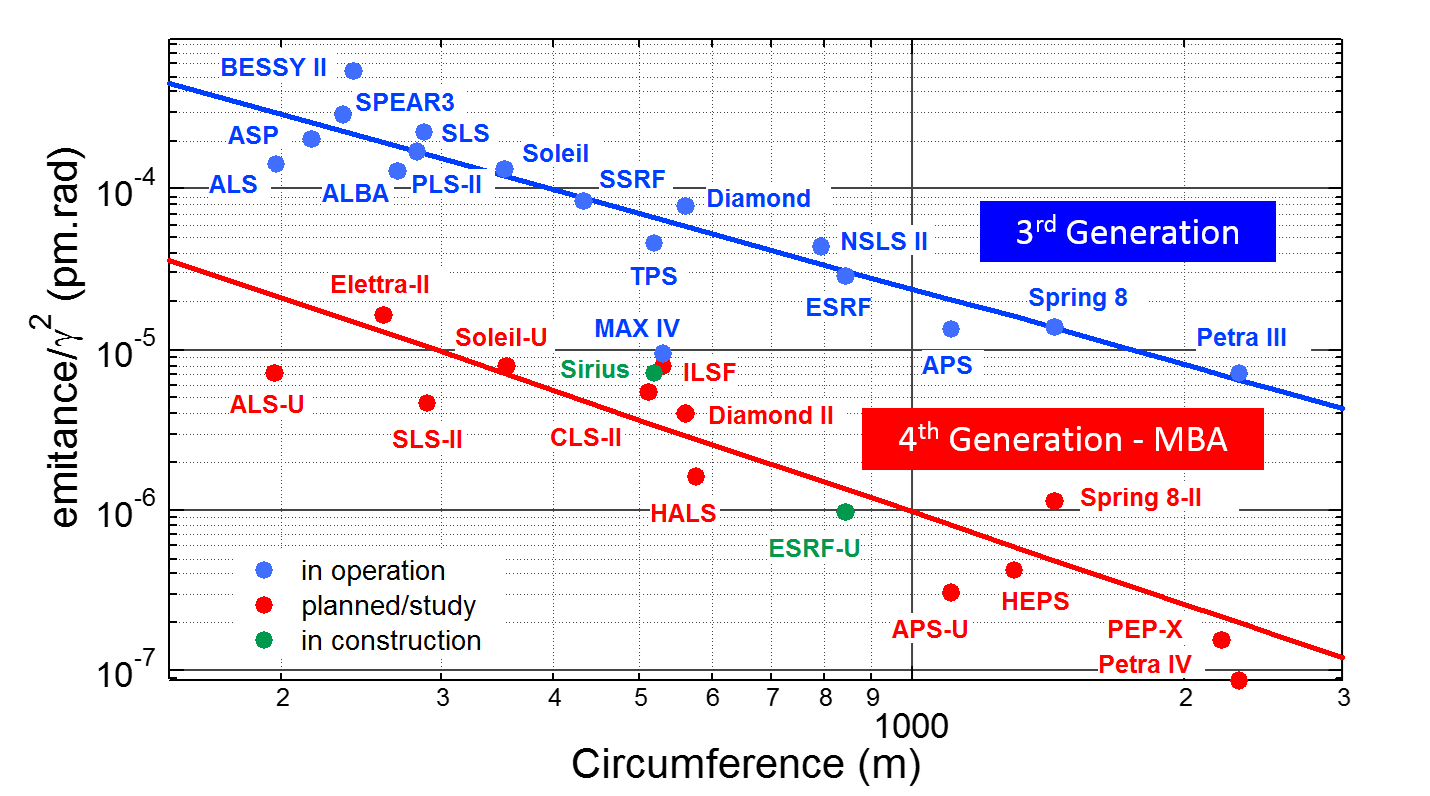
\includegraphics[width=\textwidth]{emittance_third_versus_fourth.png}
        \caption[Comparison of machines emittances.]{Natural emittance normalized by relativistic energy square as function of ring circumference for several existing \gls{3gls} and future \gls{4gls}. The blue solid line is a fitting among the \gls{3gls} and the red solid line is a fitting among the \gls{4gls}. Notice the only \gls{4gls} in operation is MAX-IV. Adapted from~\cite{Liu2017}.}
        \label{fig:scaled_emittances}
    \end{figure}
    where $\gamma = E/m_0c^2$ is the relativistic energy and $N_b$ is the number of dipoles, or bending magnets, of the storage ring. Besides, higher energy storage rings generally imply in larger circumferences and, consequently more dipoles. Given the scaling presented above, it is clear that in general the emittance is reduced with the increase of the ring circumference, as shown by the tendency lines in the figure.

\subsection{\Glsentryfull{mba}}

    The main reason for the \gls{4gls} to achieve such small emittances is the use of \gls{mba} lattices. In \gls{3gls} the number of dipoles in one unit cell of the magnetic lattice is two or three depending on the machine, but in \gls{4gls} this number is larger than five, hence the name multi-bend. The achromat part of the name \gls{mba} is due to the fact that energy dispersion errors introduced by dipoles are corrected locally and do not affect the trajectories and transverse bunch sizes inside the \gls{ids}.

    Even though this change does not seem to be harmful or difficult in a first analysis, it requires several developments in almost all the areas involved in designing, constructing and operating a light source~\cite{Liu2017,Neuenschwander2015,Hettel2014}. The larger number of dipoles in a short space requires strong focusing from the quadrupoles to achieve low emittances. These strong quadrupoles requires strong sextupoles to correct their chromatic errors, which, in turn, requires other strong sextupoles to increase the stability region around the fixed point of the one turn map. In order to produce all these strong magnets, they need to be closer to the beam, their gap must be smaller, which implies the vacuum chambers must be smaller too. The smaller vacuum chamber decreases the vacuum conductance\footnote{The vacuum conductance is proportional to the third power of the vacuum chamber radius~\cite{someone}.}, making it necessary to adopt different solutions for vacuum, generally distributed along the whole ring, such as the use of \gls{neg} coating inside the chambers~\cite{negcitation}. The proximity of the vacuum chamber and all the other in-vacuum components to the beam, increase the beam coupling impedance, which leads to higher heating of the components and to instabilities. The stronger magnets also implies more sensibility of the lattice to errors, such as construction errors of the magnets, misaligments and multipoles~\cite{wikilnls}, and, together with the very small transverse sizes of the beam, requires tight tolerances on ripple from the power supplies and vibration, not only of the magnets, but also of the components of the beamlines, such as the monochromators~\cite{monochromlnls}. Underlying all these intrincacies is the need of very detailed design, characterization and, in some cases measurement, of all the components that are installed in the light source. Besides, detailed single particle models of the storage ring are fundamental to evaluate the effect of every new design on the global properties of the ring, such as beam lifetime and dynamic aperture. All this requires very detailed simulations and high computational power.

    Regarding the beam coupling impedance, the last \gls{3gls} that were built already demonstrated concern to evaluate the budget of the ring, simulating and, more importantly, designing the components to minimize heating and other impedance related issues~\cite{nagaokasoleil,tomasalba,nslsii}. For \gls{4gls} this approach is practically mandatory because the predictions for thresholds for strong instabilities are much lower for these machines than they were for \gls{3gls}~\cite{heps,sirius,diamond2}. Besides, the use of ~\gls{neg} technology extended along the whole ring requires more detailed analysis of its effect on the impedance.

\section{Collective Effects}

    Collective effects can cause severe deterioration of the brightness of a machine because they can lead to the increase of the effective emittance of the electron beam, through coherent oscillations of the bunches, increase of the energy spread and the beam sizes in all three planes. Besides, they can even cause beam loss, which limits the maximum current that can be stored and consequently the total photon flux of the machine. In this section we will introduce the main mechanisms that drive collective effects in a storage ring.

\subsection{Interaction Mechanisms}

    One of the most important interaction for storage rings of light sources is the collision of particles, generally refered to as Coulomb scattering or intrabeam scattering, which is so unpredictable and chaotic that its effects on the beam resembles the properties of the emission of radiation, causing emittance and energy spread increase~\cite{intrabeam_scaterring}. Additionally, the collision process also leads to particle loss through a mechanism called Touscheck scattering~\cite{touscheck_scatering}, where the transverse energy of oscillation is transfered to the longitudinal plane and the particles gain an energy deviation so large that they are lost. All these effects are very detrimental to new light sources, being the Touscheck lifetime their main source of particle loss~\cite{touscheck_lifetime}.

    The \gls{dsp} is another type of interaction among the particles, being the result of the action of the cloud of electromagnetic field existent inside the beam on individual particles. Each particle generates an electric and a magnetic field that, when averaged among all particles, result in a net potential dependent on the shape and sizes of the bunch. This potential acts like an external field on the movement of the particles, leading to tune-shifts with amplitude and possible excitation of resonances~\cite{direct_space_charge}. However, for ultra-relativistic electron beams such as the ones of a light source storage ring, with energies of the order of a few \si{\giga\electronvolt}, this effect is very small and can be neglected. This happens because in this limit the non-radiating fields generated by each particle is concentrated in a plane transverse to its movement and the electric and magnetic forces that act on other particles moving parallel to it cancel each other out. In Appendix~\ref{app:lorentz_cancel} a more detailed explanation for this property is given.

    The \gls{csr} is another type of direct interaction between particles in a beam. The radiation emitted by the particles travels forward with the velocity of light and, due to the fact that the particles are moving on a curved trajectory when they emit light, this radiation catches up with the particles ahead of the emitting particle. If the wavelength of the radiation is of the same order of or larger than the bunch length, the average of this effect is non-zero and the head of the bunch feels a net force. As this effect depends on the radiated field, in contrast to the \gls{dsp}, it does not tend to zero as the energy of the particles increases and can be very harmful, depending on the bunch length of the beam, causing energy spread increase and bunch lengthening or even microbunching~\cite{csr_instability}. However, this mechanism of interaction suffers from shielding of the vacuum chamber because, depending on the transverse separation of the walls, the low frequency radiation cannot propagate, which mitigates the effect~\cite{csr_shielding}.

    All mechanisms described above are examples of direct interactions among the particles, they do not depend on the environment in which they are imerse to happen. The wake fields and the \gls{isp} on the other hand, use the vacuum chamber as intermediary of the interaction. The contact of the non-radiating field of the beam with the metallic walls of the chamber induces currents in the surface of the metal that travels with the beam, these surface currents also generate an electromagnetic field that propagates to the center of the vacuum chamber and influences the movement of the particles. This electromagnetic field can have properties of non-radiating and radiating field, depending on the characteristics of the vacuum chamber. If we consider the chamber is perfectly conducting and with translational symmetry in the longitudinal direction, then the surface charges travel in straight lines with the beam speed, which means they will produce only non-radiating fields with the same properties of those of the \gls{dsp}. This is the origin of the \gls{isp}, that for the same reasons as the \gls{dsp} is negligible for high energy storage rings.

\subsection{Wake Fields}\label{ssec:wake_fields}

    If any of the two conditions imposed on the vacuum chamber is broken, then the surface charges also generate radiating fields or fields that are dragged behind the source particle, namely wake fields. For example, if the vacuum chamber has no longitudinal translational symmetry, then the surface charges must follow curved paths, which makes then suffer accelerations and hence, radiate electromagnetic fields. Notice that this is only one of the several possible ways of introducing this mechanism, it would be equivalent to say that the surface of the metal scatter the fields generated by the particles in the beam and when the surface of the vacuum chamber has longitudinal symmetry the refletion is specular but when it has corrugations or transitions, the scattering is difuse. Precisely what happens is that the walls of the vacuum chamber impose \gls{bcon} on the fields that exist inside the vacuum vessel, univocally defining its time and spatial dependency.

    The wake fields can be very harmful to the beam, changing the properties of the static distribution of particles and creating instabilities above a given current threshold, which can lead to coherent oscillations of the bunches, emittance and energy spread increase and even beam loss. All these effects cause serious deteriorations of the brightness of the radiation, limiting the photon flux and the deterioration of its phase space average distribution.

\section{Brazilian Synchrotron Light Laboratory}

  	The \gls{cnpem} is a brazilian institution located in Campinas-SP that gathers four national laboratories, being the \gls{lnls} one of them. This laboratory was created in 1987 with the objectives of to project, construct and operate a \gls{sls}. Such goals were successfully achieved with UVX, a second generation light source which begun operation with external users in 1997. Since them the brazilian community of synchrotron users has grown and studies of a new, more competitive machine, started in 2008.

\subsection{Sirius}

    By the end of 2011, Sirius was a well developed project and it consisted on a permanent magnet based \gls{3gls}, with an energy of \SI{3}{\giga\electronvolt}, an emittance of the order of \SI{2}{\nano\meter\radian} and circumference of \SI{480}{\meter}~\cite{SiriusAntigo}. This scenario changed after the first reunion of the \gls{mac}, in june of 2012, when the committee inspired the project leaders to follow the example of MAX-IV~\cite{MaxIVfirst} and pursue sub-nanometer emmittances. This challenge was accepted and Sirius became the second project to fit the category of what today is called \gls{4gls}~\footnote{At the begginning these machines were called "The Ultimate Light Sources" and then "Diffraction Limited Light Sources". But as the initial excitement of the community faded away the names became more humble and today it seems they have converged to "4th Generation Light Sources".}, with a natural emittance even lower than MAX-IV's~\cite{FirstSirius}.

    After several changes in the magnetic lattice~\cite{ipac2014,ipac2015} to improve the brightness of the light generated by the insertion devices that were being planned for Sirius~\cite{wikisirius,luana}, the current lattice of the storage ring is the one presented in Figure~\ref{fig:sirius_lattice}.
    \begin{figure}[t!]
        \center
        % 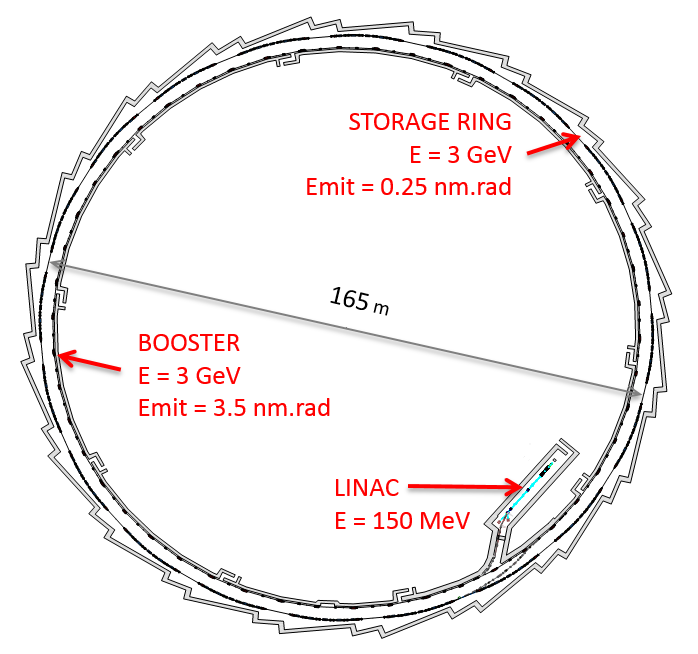
\includegraphics[width=0.7\textwidth]{sirius_machine.png}
        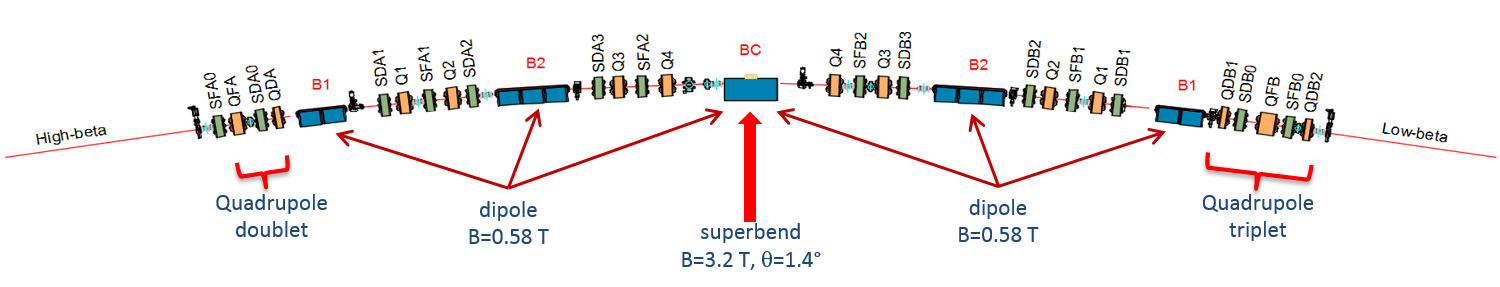
\includegraphics[width=\textwidth]{sirius_lattice.png}
        \caption[One fourth of the unit cell of the Sirius storage ring.]{One fourth of the unit cell of the Sirius storage ring. Dipoles are shown in blue, quadrupoles in orange and sextupoles in green. The vacuum pumps and valves are also shown. Only half of the high-beta (A) and of the low-beta (B) straight sections are shown. The arc and the straight sections are repeated to form the unit cell in the following way: A-B-B-B. The unit cell is then, repeated five times to form the ring.}
        \label{fig:sirius_lattice}
    \end{figure}
    The arc of the cell, composed of all the elements from the first to the second B1 dipole, inclusive, is repeated twenty times to form the ring. The straight sections alternate in sections with two quadrupoles (A), and sections with three quadrupoles (B), in the following manner: A-B-B-B, in such a way that the ring has five A sections and fifteen B sections. The difference between these two types of sections is that beam is strongly focused in the B sections, to improve the radiation generated by the undulators which will be installed there and the A sections are optimized for the injection from the booster, that will take place in one of them. These way the ring has twenty straight sections, from which eighteen will be available for installation of \gls{ids}. However the real symmetry of the ring is only five, which difficults the optimization of the single particle non-linear optics~\cite{Sa2016, Dester2017}. In the center of each arc there is a special dipole magnet, with longitudinal gradient and a very strong peak field of \SI{3.2}{\tesla} in its center that will provide hard x-rays, with critical energy of \SI{19.2}{\kilo\electronvolt}, for additional 20 beamlines~\cite{Liu2016, wikisirius}.

    The whole accelerator complex of the Sirius \gls{sls} will be composed of a \SI{150}{\mega\electronvolt} \gls{linac}, a full range booster synchrotron, that will ramp the electrons from the \gls{linac} energy to the storage ring nominal energy with a cycling rate of \SI{2}{\hertz}, and the storage ring. The injection system will operate in topup mode, where the total current of the storage ring is kept constant along the whole operation shift, because periodic injections cycles along the day are performed without the need of interrupting the operation of the machine. The booster will be concentric to the storage ring and placed inside the same tunnel, which minimizes costs related to the construction of a separate shielding and helps diminishing its emittance, only \SI{3.5}{\nano\meter\radian} at \SI{3}{\giga\electronvolt}, which is important to maximize the injection efficiency in the storage ring.

    Table~\ref{tab:sirius_main_parameters} shows the main global parameters of the storage ring and Table~\ref{tab:sirius_operation_phases} shows the predicted operation phases of the machine along the next years. Even though the commissioning will be performed with a normal conducting PETRA 7-CELL RF cavity, in the users operation phases the RF cavities of the storage ring will be superconducting. It is predicted the installation of a 3th harmonic passive landau cavity to lengthen the bunches and increase the lifetime, allowing multi-bunch operation with higher currents. There is no prediction of operation with single bunch, but high single bunch current in the middle of the train is foresaw. Even though the expected filling of the machine is the uniform shape, it is possible the need of operating with gaps due to ion instabilities~\cite{ioninstability}.

    \begin{table}[b]
        \caption{Main Parameters of the Sirius Storage Ring.}
        \begin{subtable}[h]{0.45\textwidth}
            \centering
            \caption{example table.}
            \label{tab:sirius_main_parameters}
            \begin{tabular}{c|c|c}
                1&2&3\\
                4&5&6
            \end{tabular}
        \end{subtable}
        \begin{subtable}[h]{0.45\textwidth}
            \centering
            \caption{example table.}
            \label{tab:sirius_operation_phases}
            \begin{tabular}{c|c|c}
                1&2&3\\
                4&5&6
            \end{tabular}
        \end{subtable}
    \end{table}

\section{Description of the work}

    The first objectives of this work were to study the subject of wake fields and impedances in accelerators and their effects on the beam dynamics of electron storage rings. The following goals were to apply this knowledge gathered from the literature to the Sirius storage ring, building the impedance budget with semi-analytical and numeric calculations of the impedances of the main components of the storage ring\footnote{This part of the work was shared with other members of the \gls{lnls} team.}, with special care to the characterization of the effect of the \gls{neg} coating on the total impedance; and to perform calculations to predict the beam instabilities thresholds and study the possible cures for them.

    This thesis is organized in the following manner: in Chapter~\ref{cap:single_particle_dynamics} the main concepts of the single particle dynamics, important for the development of the rest of the work, will be introduced; in Chapter~\ref{cap:wakes_impedances} the main aspects of the wake field theory will be presented with focus to the physical interpretation of the quantities introduced; in Chapter~\ref{cap:collective_effects} the methodology for computation of the impedance effects on the beam will be briefly described, with references for more detailed works and explanation of the derivation of the equations; in Chapter~\ref{cap:impedance_modelling} the models applied to the impedance calculation of the main components of the storage ring will be presented and justified;


%%%%%%%%%%%%%%%%%%%%%%%%%%%%%%%%%%%%%%%%%%%%%%%%%%%%%%%%%%%%%%%%%%%%%
%%%%%%%%%%%%%%%%%%%%%%%%%%%%%%%%%%%%%%%%%%%%%%%%%%%%%%%%%%%%%%%%%%%%%
\chapter{Single Particle Dynamics}\label{cap:single_particle_dynamics}

    In this chapter the main concepts of single particle dynamics that will be useful for the rest of the work will be introduced without any intention to be complete or rigorous in the presentation. There are great books~\cite{LeeBook,WiedemannBook} and also some outstanding reports~\cite{Sands1969Int} that cover all the topics presented here, and much more, with incredible didactic.

\section{Reference System}

    Connected to the concept of a storage ring is the one of the reference orbit. This special closed orbit is the one that an idealized particle, the synchronous particle, with the storage ring nominal energy would follow if it had the correct initial conditions. Besides, all the components of a storage ring are aligned according to this special orbit in such a way that their center, symmetry points or axis coincide with it and, in practice, the trajectories of all particles stored in the machine will be close to it. For this reason, the reference orbit is chosen to be the origin of the reference frame, defining a curved coordinate system that moves along the ring, with one longitudinal coordinate tangent to the local orbit and two transverse coordinates perpendicular to it. This type of co-moving coordinate system is a particular case of a Frenet-Serret frame~\cite{Frenet1847,Serret1851,wikipedia}, where the torsion is always zero, due to the fact that storage rings only have dipoles to bend the trajectories in the horizontal plane. Such a coordinate system can be defined in the following way~\cite{LeeBook}:
    \begin{align}\nonumber
        \versor{s}(s) &= \dertot{\vect{r}_0(s)}{s},\\
        \versor{x}(s) &= -\rho(s)\dertot{\versor{s}(s)}{s},\\\nonumber
        \versor{y}(s) &= \versor{s}(s) \times \versor{x}(s),
    \end{align}
    where $s$ is the arc length of the reference orbit starting from an arbitrary point, $\vect{r}_0$ is the position of the reference orbit in relation to a static, cartesian reference frame, $\versor{s}$ is the vector tangent to the orbit, standard from the Frenet-Serret description, $\versor{x}$ is the negative of the normal vector, generally called in accelerator physics as radial or horizontal coordinate, $\versor{y}$ is the standard binormal versor, often called as vertical direction in accelerator physics. The scalar $\rho$ is the local radius of curvature of the reference orbit, which is equal to the one introduced by the dipoles, as defined in equation~\eqref{eq:curvature_dipole}. This means that the reference frame of an accelerator is piecewise straight with curvature different from zero only at the dipoles.

    With the definitions above, the position of an arbitrary particle can be described as small deviations from the reference orbit (see Figure~\ref{fig:reference_frame})
    \begin{align}
        \vect{r}(s) = \vect{r}_0(s) + x\versor{x}(s) + y\versor{y}(s)
    \end{align}
    \begin{figure}
        \centering
        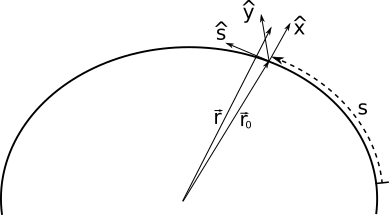
\includegraphics[width=0.65\textwidth]{coordinate_system.png}
        \caption[Frenet-Serret reference frame of a storage ring]{Frenet-Serret reference frame of a storage ring, with right-handed coordinate system $\{ \versor{x}, \versor{y}, \versor{s} \}$. Adapted from~\cite[pp. 123]{LeeBook}.}
        \label{fig:reference_frame}
    \end{figure}
    with $x$ and $y$ being the horizontal and vertical displacements of the particles in relation to the reference orbit. In this reference frame, the dynamics of each particle can be represented by its position in the six dimensional phase space defined by:
    \begin{align}\label{eq:phase_space_definition}
        \left\{ x, x', y, y', z, \delta \right\}
    \end{align}
    with
    \begin{align}
        x' = \dertot{x}{s} \approx \frac{p_x}{p_0},\quad
        y' = \dertot{y}{s} \approx \frac{p_y}{p_0},\quad
        \delta = \frac{p}{p_0}-1
    \end{align}
    where $p_0$ is the storage ring nominal linear momentum, $\delta \approx \Delta E/E_0$ is the energy deviation of the particle in relation to the nominal energy of the storage ring and $x'$ and $y'$ are the normalized transverse components of the linear momentum of the particle. The coordinate $z$ is defined as the relative longitudinal position of the particle in relation to the synchronous particle
    \begin{align}\label{eq:longitudinal_deviations}
        z(t) = s_\text{sync}(t) - s(t)
    \end{align}
    where $t$ is the wall-clock time and $s_\text{sync}(t)$ is the position of the synchronous particle. Notice if the particle is ahead of the synchronous particle then $z$ will be negative. This convention is very important and will be consistently adopted throughout this work.

\section{Transverse Dynamics}

    At this point it is convenient to describe in general terms how is the movement of the stored particles. They are ultra-relativistic electrons with energy of the order of a few \si{GeV}, and most of their velocity is always in the direction of the tangent of the ideal orbit. There are approximately hundreds of billions electrons grouped in several bunches along the reference orbit, each bunch having length of a few milimiters and transverse sizes of the order of dozens of microns. Each electron is under the influence of a variaty of electromagnetic fields (gravity can be neglected), coming from the static magnetic fields of the dipoles and multipoles, the radiofrequency field of the RF cavity, the direct fields of other electrons in the same bunch and the fields scattered by the vacuum vessel, generated by other electrons in the same bunch, in other bunches or even by themselves in previous turns. Also, they emit synchrotron radiation which makes them lose energy and perturbes their movement with a recoil effect.

    The description of the dynamics of the stored particles begin with an approximation that neglect the effects of their self-fields, i.e. their interaction with each other, with the vacuum chamber and with the residual molecules in their atmosphere. In this framework the only forces acting on the particles are the magnetic fields of the dipoles and multipoles and the longitudinal electric field of the RF Cavity and the only way they can lose energy is through synchrotron radiation emission. Under such conditions, the one turn map of the ring defines a fixed point in the phase space defined in equation~\eqref{eq:phase_space_definition} and the particles oscillate around it, being the oscillations in the planes $\{x,x'\}$, $\{y,y'\}$ and $\{z,\delta\}$ practically uncoupled. The oscillations in the first two planes are called transverse oscillations, while the one in the third plane is denominated longidutinal oscillation.

    When such calculations are performed for current synchrotrons it is noticeable that the dynamics of the longitudinal motion is much slower than the dynamics of the transverse motion. As an example, in the Sirius storage ring particles take approximately 215 revolutions around the ring to complete one turn around the fixed point in the longitudinal direction while they oscillate 49 times per revolution around the fixed point in the transverse plane. This property makes it possible to separate the study of the longitudinal plane from the transverse one, considering the energy deviation of one particle as a constant parameter in the transverse equations of motion. The effects of the radiation energy loss are even slower than the longidudinal motion, taking a few thousands of turns in the ring to significantly change the transverse motion.

    Neglecting the energy variations of the particles, and the randonnes of the radiation emission, the motion of the particles can be described by a hamiltonean in the Frenet-Serret coordinate system defined by the ideal orbit. Procceding in the approximations, considering the paraxial motion of the particles around the closed orbit, this hamiltonean can be simplified to a quadratic form in the momenta coordinates. See, for example, the second chapter of reference~\cite[pp. 32]{LeeBook}.

    This Hamiltonean generates two second order coupled and non-linear equations of motion for the transverse coordinates that accurately describes the short and mid-term stability of the particles. Most of the non-linearities and coupling in these equations come from the magnetic fields of the magnets along the ring, being the other contributor the curvature of the reference orbit and the energy deviation of each particle. At this stage of the simplification of the problem the dynamics of the electrons still is very complicated, mainly for storage rings such as Sirius, with several and very strong Sextupoles that introduces chaos in the system in regions of the phase-space that are close to the fixed point.

\subsection{Linear Equations of Motion}

	With further approximations, considering only the terms of the equations of motion that are linear with the phase-space coordinates and eliminating all coupling between the two transverse directions, the analysis of the dynamics becomes simple enough to allow its complete understanding, with analytical solutions to the equations of motion and physically significant parametrizations, that summarizes and simply describes a given machine. In this regime, the transverse movement of the electron is only dependent on the fields of dipoles and quadrupoles. Under such considerations, the Hamiltonean of an arbitrary particle stored in the ring is given by
    \begin{align}\label{eq:approximated_hamiltonean}
        H \approx \frac{x'^2}{2} + \frac{y'^2}{2} - \frac{G^2(s)}{2}x^2 + \frac{K(s)}{2}\funcof{x^2-y^2} + G(s)x\delta
    \end{align}
    where we notice the Hamiltonean is normalized by the total momentum of the particle, $p$, and expanded up to second order in the transverse phase space coordinates, in such a way that only dipoles, $G(s)$, and quadrupoles, $K(s)$, contribute to the dynamics. Besides, the independent variable was changed from time to the longitudinal position of the particle along the Frenet-Serret frame, which is possible because $s$ is a monotonic function of the time in storage rings, which allow easy invertion of derivatives. All the steps to get the equation above are described in details in the literature~\cite{LeeBook,Bengtssonpaper,WiedemannBook}. The equations of motion will be:
    \begin{align}\label{eq:linear_equation_motion}
        x'' &= -\derpar{H}{x} = -\funcof{K(s)-G^2(s)}x + G(s)\delta\\\nonumber
        y'' &= -\derpar{H}{y} = K(s)y
    \end{align}
    where the energy deviation dependent term in the horizontal equation of motion is the dispersion generated by the dipole.

	Looking back at the beggining of this section and reviewing all the approximations, at first sight it seems that the region of validity of these linear equations is so limited that their understanding is useless. However that is not what is observed in practice, because storage rings are carefully designed to maximize the validity of this linear behavior: the position, number and strength of all magnets are so well tuned that nonlinearities cancel each other. Another important point to justify the study of these linear equations is that, luckly, for synchrotron radiation generation the smaller the transverse size and divergence of the electron beam the better, which means most particles will stay for most of the time in a very small region of approximately hundreads of microns around the fixed point, where only the linear part of the one turn map have a significant effect on the dynamics. Besides, if a particle experience large transverse oscillations and happens not to be lost, damping effects that arise due to synchrotron radiation emission will bring them close to the fixed point in a few dozens of miliseconds.

\subsection{Betatron Function and Phase Advance} \label{ssub:betatron_function}

    The homegeneous part of the equations of motion presented in equation~\eqref{eq:linear_equation_motion} can be cast in the following way:
    \begin{align}
        u'' + K_u(s)u = 0
    \end{align}
    where $u$ can be both, $x$ and $y$ and $K_x=K(s)-G^2(s)$ and $K_y=-K(s)$. These equations are known as Hill equations~\cite{HillEqu} and their solutions can be parametrized in the following form:
	\begin{align} \label{eq:betatron_motion}
		u(s) &= \sqrt{2J\beta_u(s)} \cos(\mu_u(s) - \phi)
	\end{align}
	where $\beta_u(s)$ is called the betatron function and depends only on the magnetic lattice and $\mu_u(s)$ is called phase advance and its relation to the betatron function is given by
	\begin{align}\label{eq:phase_advance}
		\mu'_u(s) &= \frac{1}{\beta_u(s)}.
	\end{align}
	The constants $\phi$ and $J$ depend on the initial conditions. It can be shown that:
	\begin{align} \label{eq:linear_invariant}
		J = \gamma_u(s)u^2(s) + 2\alpha_u(s)u(s)u'(s) + \beta_u(s)u'^2(s),
												\quad \text{with}& \\[3mm]
        \alpha_u(s) = -\frac{\beta_u'(s)}{2} \quad \text{and} \nonumber \quad
		\gamma_u(s) = \frac{1+\alpha_u^2(s)}{\beta_u(s)},
	\end{align}
	which represents the equation of an ellipse in phase space with $J$ being the area of such ellipse.

	The relevance of this parametrization is that there are several very important practical informations regarding the properties and responses to perturbations of the beam that can be extracted directly from the betatron function. It can be seen from equation~\eqref{eq:betatron_motion} that the maximum excursion a given particle can experience in a fixed longitudinal point of the ring is proportional to the square root of the betatron function. Analogously, the beam size of a distribution in equilibrium will also be proportional to the square root of the local betatron function. Thus, the ratio between the amplitudes of movement in two different positions is proportional to the ratio of the square root of the betatron functions at the two locations, a property that is fundamental in the process of defining the transverse sizes of the vacuum chamber of a storage ring. For example, lets suppose the maximum betatron function of a lattice is \SI{16}{\meter} and at this place the vacuum chamber has an internal dimension of \SI{12}{\milli\meter}. This means that in another place where the betatron function is only \SI{1}{\meter} the vacuum chamber can be much smaller, only \SI{3}{\milli\meter}, without affecting the stored beam, which would allow the installation of devices that requires smaller appertures. This strategy of focusing the betatron function is commonly used in storage rings in straight sections where \gls{ids} are installed, with smaller gaps they can generate stronger magnetic fields, which is desirable for radiation emission.

	Another important property that can be infered from the betatron function is the sensibility of the beam to spurious eletromagnetic fields. It can be shown that the larger the betatron function the larger the effect of such field in the beam dynamics. In the special case of dipolar fields, which are constant in the transverse plane, this dependency goes with $\sqrt{\beta(s_0)}$, for a quadrupolar field it is proportional to $\beta(s_0)$, for a sextupole $\beta^{3/2}(s_0)$ and so on.

	Besides the betatron function, another important advantage of the parametrization presented in equation~\eqref{eq:betatron_motion} is the interpretation of the integral of the phase advance in one turn around the ring. This integral normalized by \SI{2\pi} defines the tune of the machine:
	\begin{align}
		\nu_u = \frac{1}{2\pi}\udefoint{s}{\frac{1}{\beta_u(s)}}.
	\end{align}
	The integer part of this number corresponds to the number of complete oscillations in the phase space the particles make in one turn in the ring. To interpret the fractional part it is important to notice in equation~\eqref{eq:betatron_motion} that the movement of a particle in a fixed longitudinal position in sucessive turns is a perfect senoid, independently of the parametrization:
	\begin{align}
		u_i(s_0) = A_{u,0}\cos(2\pi\nu_u i -\phi_0).
	\end{align}
	where $A_{u,0}$ is a constant and the fractionary part of the tune is identified as the natural frequency of oscillation. This means that resonances can be excited by any electromagnetic field along the ring with a frequency equal to the tune times the revolution frequency. This is the main mechanism that drives the collective instabilities that will be studied in this work. The electromagnetic fields generated by a bunch of particles interacts with other bunches and, because they have the same oscillation frequency, which is the tune, a collective oscillation emerges due to resonance. This can even happen in a single bunch, where oscillations of the head of the bunch drives the tail to ever larger oscillations.

	Additionally, resonances can even be excited by static fields if the tune is a rational number, as long as these fields have the correct transverse spatial dependency. For example, if the fractionary part of the tune is $\sfrac12$ and there is a spurius constant quadrupolar field in some point of the ring, the kicks received by the particles in successive turns would always sum constructively and a resonance behaviour would be excited. If both transverse planes of motion are considered it can be shown that if the tune satisfies the equation:
	\begin{align}\label{eq:betatron_resonance}
		m\nu_x + n\nu_u &= p
	\end{align}
	where $m$, $n$ and $p$ are integers, resonances can be excited depending on the static magnetic field around the ring. The number $r^2 = m^2 + n^2$ is called the order of the resonance, and the lower the order the higher its strength. If both, $m$ and $n$ must be non-zero for the equation~\eqref{eq:betatron_resonance} to be true, then the resonance depends on the existence of coupling fields, where the position of the particle in one direction influences the kick in the other direction.

\subsection{Dispersion Function}

	The inomogeneus solution of the linear equations of motion can be written in the following form:
	\begin{align}\label{eq:dispersion_function}
		x_\delta(s) = \eta(s)\delta
	\end{align}
	where $\eta(s)$ is called dispersion function and, just like the betatron function, depends only on the magnetic lattice. Notice that this is a particular solution of the equation, where periodic conditions were applied. This choice has an advantage over other solutions because of the meaning of the dispersion function: its value along the ring give the shape of the averaged trajectory of a particle with non-zero energy deviation. In other words, this particular solution of the inomogeneus equation gives the closed orbit of off-momentum particles.

	The dispersion function is very important to determine the equilibrium emittance of a storage ring~\cite[pp. 304]{WiedemannBook},
    \begin{align}
        \varepsilon_0 \propto \udefoint{s}\frac{\mathscr{H}\funcof{\eta(s),\eta'(s)}}{\rho^3(s)}
    \end{align}
     where the minimization of the functional
	\begin{align}
		\mathscr{H}(\eta(s), \eta'(s)) &= \gamma_x(s)\eta^2(s) +
										2\alpha_x(s)\eta(s)\eta'(s) +
										 \beta_x(s)\eta'^2(s)
	\end{align}
	in the dipoles of the ring is one of the main goals when designing a storage ring. Besides, the dispersion function is important to calculate the momentum compaction factor, $\alpha$, which is the relative difference in path length in one turn in the ring per unit of energy deviation:
	\begin{align}\label{eq:momentum_compaction}
		\frac{\Delta L}{L} &\approx \delta \alpha \coloneqq \delta \udefoint{s}{\frac{\eta(s)}{\rho(s)}}.
	\end{align}
	This parameter, which in general is positive, is of fundamental importance for the longitudinal dynamics, because it couples linearly the time it takes for the particles to complete one turn in the ring with their energy deviation. Notice that the only sections of the ring which contribute to the integral are where the reference orbit is curved (in other places the radius is infinity) and this is because particles with more/less energy generally follow paths with larger/smaller radius in the dipoles, which increases/decreases the path lenth. Negative momentum compaction are possible to be obtained in several storage rings by adjusting the quadrupoles of the lattice, but these mode of operations are rare and in the case of Sirius it will not be possible to operate under such condition.

\subsection{Action-Angle Variables}

    Finding the action angle variables for a given Hamiltonean is equivalent to solve the equations of motion, due to the simple time, or $s$, evolution of such variables. For  hamiltoneans with one elliptic fixed point, this task is achieved by performing canonical transformations in the phase space variables that brings them to the normal form, where the movement is a simple harmonic oscillator. Then, the radius in phase space is an invariant of motion and is recognized as the action. This procedure can be applied to the Hamiltonean of equation~\eqref{eq:approximated_hamiltonean} by recognizing the dispersion orbit as a canonical transformation that changes the origin of the phase space~\cite[Appendix A2]{Berg1996}
    \begin{align}\label{eq:off_momentum_canonical_transformation}
        x (s) \to \overbrace{x(s) - x_\delta (s)}^{x_\beta},
    \end{align}
    where $x_\delta (s)$ is given by equation~\eqref{eq:dispersion_function}, in such a way that the new Hamiltonean is purely a quadractic form, without the crossed term $x\delta$. This pure betatronic Hamiltonean can than easily be written in action-angle variables in the following way:
    \begin{align}\label{eq:betatron_hamiltonean}
        K = \frac{J_x}{\beta_x(s)} + \frac{J_y}{\beta_y(s)}
    \end{align}
    where $J_x$ and $J_y$, defined by equation~\eqref{eq:linear_invariant} are recognized as horizontal and vertical actions and the equation of motion shows that the angle variable, $\theta$, is the phase advance, defined in equation~\eqref{eq:phase_advance}:
    \begin{align}
        J'_u = \derpar{K}{\theta_u} = 0 \quad \text{and} \quad \theta'_u = \derpar{K}{J_u} = \frac{1}{\beta(s)} = \mu'_u
    \end{align}
    These variables will be very important for this work, because the wake-fields will be included in the electron dynamics as perturbations to the Hamiltonean presented above.

\subsection{Linear Map Formulation: Matrix Theory}

	An alternative way to describe the linear dynamics of a storage ring is via symplectic transfer matrices, where the evolution of the coordinates in phase space can be always written in the following form
	\begin{align}
		\vect{u}(s) = \tensor{M}_{s_0\to s} \vect{u}(s_0)
	\end{align}
	where $\vect{u}(s) = \left(u(s), u'(s)\right)$ is the coordinates in phase space and  $\tensor{M}_{s_0\to s}$ is the transfer matrix from points $s_0$ to $s$. This form of the time evolution of the coordinates can be obtained from equation~\eqref{eq:betatron_motion} by derivation with respect to $s$ and substitution of $J$ and $\phi$ by the initial conditions $\vect{u}(s_0)$. After this procedure, it can verified that $\vect{M}$ can be written in normal form~\cite{bengtsson}
	\begin{align}
		\tensor{M}_{s_0\to s} = \tensor{A}(s)\cdot\tensor{R}(\mu_{s_0\to s})\cdot\tensor{A}^{-1}(s_0)
	\end{align}
	where $R$ is a rotation matrix and $A^{-1}$ is a transformation matrix to the normalized coordinates, given by
	\begin{align}
		\tensor{R}(\theta) =
				\begin{bmatrix}
					\cos(\theta)  & \sin(\theta)\\
					-\sin(\theta) & \cos(\theta)
				\end{bmatrix}
				\quad\text{and}\quad
		\tensor{A}(\mu) =
				\begin{bmatrix}
					\sqrt{\beta_u}                 & 0\\
					-\frac{\alpha}{\sqrt{\beta_u}} & \frac{1}{\sqrt{\beta_u}}
				\end{bmatrix},
	\end{align}
	and also satisfy the composition rule
	\begin{align}
		\tensor{M}_{s_0\to s_2} = \tensor{M}_{s_1\to s_2}\cdot\tensor{M}_{s_0\to s_1}
	\end{align}
	where $\{s_0, s_1, s_2\}$ in this order are sequential positions along the ring. Besides, successive turns around the ring at some position $s_0$ are completely described by the one turn matrix, $\tensor{M}(s_0)$ :
	\begin{align}
		\vect{x}_n = \tensor{M}^n \cdot \vect{x}_0, \quad \text{with} \quad
		\tensor{M}^n = \tensor{A}\cdot\tensor{R}^n(2\pi\nu)\cdot\tensor{A}^{-1} =
					    \tensor{A}\cdot\tensor{R}(2\pi n \nu)\cdot\tensor{A}^{-1}.
	\end{align}
    This formulation of the linear transverse motion is very usefull for numeric calculation of the evolution of the particles.

\subsection{Chromaticity and Action Dependent Tune-shift}

	The quadrupoles correct the chromatic effects in the orbit of the beam that are generated in the dipoles and the result of such a correction is the finite value of the dispersion function. However the quadrupoles also are dispersive components, which means their focusing strength depends on the energy of the particles. This dependency comes from higher order terms of the Hamiltonean, not shown in equation~\eqref{eq:approximated_hamiltonean}, and causes an effect on the beam where particles with different relative energy offset have different tunes.

    The linear part of this dependency is called linear chromaticity, which, if not corrected, reduces the lifetime of the beam to a few seconds in most storage rings. For example, for the case of Sirius the chromaticity of the ring without sextupoles is $\approx -130$ for the horizontal direction. This means that particles with an energy deviation of only \SI{0.15}{\percent} would have a tune that is \SI{0.2}{} smaller than the tune of a particle with zero energy deviation. As the energy deviation oscillates in the scale of hundreds of turns, this particle would almost certainly cross a resonance that would induce its loss. Considering the equilibrium energy spread of the Sirius storage ring is only half of this value, $\approx$ \SI{0.09}{\percent}, without chromaticity correction all particles with energy deviation above two sigma of this distribution would be lost.

	The sextupoles are introduced in the machine to correct the linear chromaticity to values close to zero. In this processes of minimization they change the higher-order chromatic terms and also introduce geometric aberrations, non-linearities in the dynamics of all particles that reduces the region around the fixed point where the beam is stable. The main contribution of this effect for the dynamics in the vicinity of the fixed point is the generation of a linear dependency of the tune of each particle with its action variable, $J_u$. Writting the linear expansion of the tune as a function of the energy deviation and the action we get:
	\begin{align}
		\nu_x(\delta, J_x, J_y) \approx \nu_{x,0} + \xi_x \delta + A_{xx} J_x + A_{xy} J_y \\\nonumber
		\nu_y(\delta, J_y, J_x) \approx \nu_{y,0} + \xi_y \delta + A_{yy} J_y + A_{yx} J_x
	\end{align}
	where $\xi_x$ and $\xi_y$ are the horizontal and vertical chromaticities, and $A_{xx}$, $A_{yy}$ and $A_{xy}=A_{yx}$ are the action dependent tune-shifts.

\section{Longitudinal Dynamics}

    In the study of the transverse dynamics the time scale involved was of a few turns in the storare ring, which allowed us to treat the energy deviation of the particles as another constant of motion. In this section the dynamics of the electrons in a few hundreads of turns will be analysed. In this scale the transverse betatron oscillations are averaged out and the longitudinal dynamics, which describes the path length and energy oscillations around the fixed point, has its natural frequency. The main factors that influence the movement in this scale are the small unballances between the energy loss of the particles and their energy gain in the RF cavity in one turn and the revolution time variation due to the energy offset of the particles.

\subsection{Changes in Revolution Time}\label{sec:longitudinal_deviations}

    When the energy of a particle changes, its velocity is also modified, which contributes to the change of the revolution time. For most storage rings of \gls{sls}s this effect is negligible when compared to the change in path length described by equation~\eqref{eq:momentum_compaction}, due to the ultra-relativistic regime in which these machines operate. This allows us to approximate the \gls{lhs} of equation~\eqref{eq:momentum_compaction} to the relative change in revolution time. Then, from one turn to another, the relative position of a particle will change by:
	\begin{align}\label{eq:revolution_time_variation}
		z_{n+1} = z_n + \delta_n\alpha L_0
	\end{align}
	where $n$ refers to the current turn and $n+1$ to the next and $L_0$ is the nominal circumference of the ring.

\subsection{The Energy Balance}

	It can be shown that the rate of energy loss of a particle due to synchrotron radiation emission is proportial to the square of the magnetic field times the square of its total energy~\cite[pp. 123]{Jackson}. Translating this dependency to a storage ring, the energy loss in one turn depends on the magnetic lattice and on the energy deviation of the particle. For the ideal particle the energy loss is always the same and depends only on the magnetic field of the dipoles, but as the closed orbit for particles with non-zero energy deviation is different, its energy loss will be different not only because of the intrinsic dependence of the emission but also because of the slightly different magnetic fields it will experience in one turn. The combination of these effects can be modelled in the following linear approximation:
	\begin{align}\label{eq:radiation_loss}
		\Delta E_\text{Rad} \approx -U_0 - E_0L_0\alpha_z\delta_n
	\end{align}
	where $U_0$ is the energy loss of the ideal particle in one turn, $E_0$ is the nominal energy of the storage ring and the coefficient $\alpha_z$ includes both effects, the intrinsic dependence on the energy and the different orbit fields.

	The energy gain of a particle in the RF cavity is given by the integral of the longitudinal electric field, $E_\parallel$, along the path of the particle and depends only on the initial phase of the field when it enters the cavity:
	\begin{align}
		\Delta E = V(t_0) = q\defint{s}{E_\parallel(s,t)|_{t=\sfrac{s}{c}+t_0}}{0}{L_c}
	\end{align}
	where $V(t_0)$ is called the gap voltage of the cavity and $L_c$ is its length.

	Now lets assume the frequency of oscillation of the electromagnetic field inside the cavity, $\omega_{RF}$, is exactly a multiple of the revolution frequency of the synchronous particle, $\omega_0$:
	\begin{align}\label{eq:harmonic_number}
		\omega_{RF} &= h\omega_0
	\end{align}
	where $h$ is called harmonic number. With this assumption, even though the fields are time dependent, the synchronous particle will always see the same conditions as it enters in the cavity. Now lets make a further assumption that the synchronous particle reaches the cavity in the exact time where it gains $U_0$ energy of the cavity:
	\begin{align}\label{eq:synchronous_phase_condition}
		V(0) = U_0
	\end{align}
	where the time reference on \gls{lhs} is relative to the position of the synchronous particle. Considering both assumptions and combining the energy gain in the cavity with the energy loss in one turn, given by equation~\eqref{eq:radiation_loss}, we get the following one turn energy balance for a storage ring:
	\begin{align}\label{eq:energy_balance}
		\delta_{n+1} = \delta_n - L_0\alpha_z\delta_n + \frac{V(z_{n+1})-U_0}{E_0}.
	\end{align}
	where the subscript $n+1$ in the particle position means that it will go around the ring first and then pass through the cavity.

\subsection{Phase Stability Principle}

	Combining equations~\eqref{eq:revolution_time_variation}~and~\eqref{eq:energy_balance} we get the one turn map for the longitudinal plane for which the synchronous position and the nominal energy defines a fixed point. To analyse the stability of this fixed point let's linearize the map in its vicinity:
	\begin{align}\label{eq:longitudinal_linear_map}
		\begin{bmatrix} z_{n+1} \\ \delta_{n+1}\end{bmatrix} = \overbrace{
			\begin{bmatrix}
                1 & \alpha L_0 \\
                -V'_0 & 1-L_0\alpha_z - V'_0\alpha L_0
            \end{bmatrix}
		}^M \begin{bmatrix} z_n \\ \delta_n \end{bmatrix}.
	\end{align}
	where $V'_0$ is the derivative of the voltage gap in relation to the arrival time of the particles at the synchronous position normalized by the nominal energy of the ring, $E_0$. The stability condition, $\text{Tr}(M) <= 2$~\cite[pp. 123]{LeeBook}, requires the derivative of the gap voltage to be positive if $\alpha$ is positive. To ilustrate this condition consider that initially a particle arrives ahead of the synchronous particle, the positive derivative means it will gain more energy, which makes it take longer to go around the ring, diminishing the difference in arrival time for the next turn. This way all particles remain in an oscillatory movement around the fixed point with frequency given by
	\begin{align}
		\text{Tr}(M) = 2\cos(2\pi\nu_s) \approx 2-(2\pi\nu_s)^2 \implies
		\nu_s \approx \frac{1}{2\pi}\sqrt{L_0\alpha_z+V'_0\alpha L_0},
	\end{align}
	where $\nu_s$ is called synchrotron tune in analogy to the betatron tunes defined in subsection~\ref{ssub:betatron_function}.

	Additionally, the determinant of the one turn matrix is $(1-L_0\alpha_z)$, which implies the oscillations are damped, with $\alpha_z$ being the damping factor. In most storage rings this effect is small compared to the oscillation time, requiring thousands of turns to influence the dynamics.

	The voltage gap has the same harmonic composition as function of the arrival time as the electric field as a function of time. This means that the condition imposed in equation~\eqref{eq:harmonic_number} implies that there are at least $h$ stable fixed point along the ring and, as in general the voltage is a pure senoid, these are the only stable points. This means that it is possible to store up to $h$ aglomerations of electrons, called bunches, in a storage ring.

\subsection{The Potential Well}

	There is an important approximation to the map equations derived in the previous sections that consists in considering the turn by turn iterations as inifinitesimal transformations and taking the limit to the continuum, considering differences between turns as derivatives. With this considerations, the equations of motion becomes:
	\begin{align}
		\dertot{z}{s} &= \alpha \delta(s) \\\nonumber
		\dertot{\delta}{s} &= \alpha_z\delta(s) + \frac{V(z(s))-U_0}{L_0E_0}.
	\end{align}

    If the damping term is not considered, the equations of motion can be derived from a static Hamiltonean, given by:
	\begin{align}\label{eq:longitudinal_hamiltonean}
		H_\parallel = \frac\alpha2\delta^2 \quad \overbrace{-
                            \defint{w}{\frac{V(w)-U_0}{L_0E_0}}{0}{z}
                        }^{U(z)}
	\end{align}
	where the first term of the \gls{rhs} is the kinetic term and $U(z)$ is called the potential well, in an analogy with a potential energy. When the oscillations are small the potential well can be expandend in power series of the longitudinal position. Generally the RF cavity of storage rings are adjusted with each other in such a way that their potentials always sum constructively, creating a practically linear potential $V(z)$ around the fixed point, which implies the Hamiltonean can often be approximated by
    \begin{align}
        H_\parallel = \frac\alpha2\delta^2 + \frac{V'}{2L_0}z^2
    \end{align}
    which is an harmonic oscillator, equivalent to the to the linear map of equation~\eqref{eq:longitudinal_linear_map}, if the damping is not considered. This harmonic Hamiltonean is often used for analytical treatments of instabilities because it is a good approximation for most RF systems and also due to the simple expressions of its action-angle variables.

\section{Radiation Damping and Equilibrium Parameters}

    The synchrotron radiation emission is a quantum process that happens uncorrelatedly among all the electrons in the beam. While the average emission has a well defined and smooth behavior, such as the spectra that are calculated with classical electrodynamics for dipoles and \gls{ids}, a closer look into the individual emissions reveals the random nature of these events. As expected the effect this process generates on the beam is also dual, the average emission is responsible for energy loss and damping of the longitudinal and transverse oscillations, while the single emission events generates uncorrelated motion in all planes that heat up the beam.

    Both effects have very different dependency on the parameters of the particles. For example, in the last section it was used that the energy loss depends linealy with the energy deviation of the particles, which caused an exponential damping of the oscillations, i.e. a damping proportional to the amplitude of the oscillation, while the heating in the longitudinal plane happens because the emissions are instantaneous and uncorrelated among electrons or in time, having no short term dependency on any parameter of the electrons, which generates random walks for the energy deviations. Because these effects have such different dependencies they always compete with each other, if the amplitude of oscillation is large the damping dominates, if it is small there is a blow up. It is this competition that generates the equilibrium energy distribution of the beam and consequently, due to the potential well, the longitudinal distribution. While the amplitude of oscillation of each electron is in an endeless variation, the average of all electrons in a bunch remains stationary, with both effects cancelling each other out.

    In the transverse plane the effect of the radiation emission on the dynamics is not as direct as in the longitudinal plane. Damping in the transverse plane is a two fold effect: first the electrons lose transverse momentum due to radiation emission because the emission is majoritarely on the direction of motion. This does not change the normalized momentum of the electron, because the longitudinal momentum is also affected by this emission. In a second moment the electron passes through the RF cavity, where the longitudinal momentum is replenished but the transverse momentum is unchanged, which means the normalized transverse momentum is decreased. The liquid effect is an exponential damping of the transverse oscillations, proportional to the betatron action of the movement.

    The excitations of oscillations happen in the horizontal plane because of the dispersion function in the dipoles. When an electron emits radiation its closed orbit abruptly changes, because its energy deviation has changed, however, as the position of the electron is the same as before, a betatron oscillation around the new closed orbit is excited. Again, both effects cancel out in the equilibrium, defining a distribution and consequently the natural emittance of the storage ring. In the vertical plane, as the dispersion is ideally zero, the excitations are created by a much weaker mechanism and the natural vertical emittance is practically zero. This mechanism is related to the fact that the photon emission is not exactly in the direction of the momentum of the electrons, but with an angle apperture around it proportional to $1/\gamma$, which slightly changes the vertical momentum of the electron, exciting betatron oscillations. In real storage rings, residual vertical dispersion function from magnet errors and coupling fields that transfer part of the horizontal emittance to the vertical plane completely dominate this process and define the vertical emittance of the beam.

\subsection{Fokker-Planck Equation}\label{ssec:fokker_planck_equation}

	All the arguments described in the last section can be mathematically described by modelling the evolution of the beam distribution in terms of the Fokker-Planck equation. In this framework we can consider the interaction of the electrons with the radiation they emit as large particles subjected to a weak random and Markovian force, with an approximately white spectrum. These are the conditions imposed on a system by the kinect theory in order for the distribution function to be described by such equation \cite{landau, Wang1945, zwanzig}.

    There are several works that explain the use of the Fokker-Planck equation in storage rings~\cite{Lindberg2016,Suzuki1983,Suzuki1986,LeeBook,Wiedemann}. Here, only the main results will be presented:
    \begin{align}\label{eq:fokker_planck_equation}
        \derpar{\Psi}{s} + \poison{\Psi, H} = \mathscr{F}\funcof{\Psi}
    \end{align}
    where $\Psi = \Psi\funcof{\vect{q},\vect{p}, s}$ is the beam distribution in phase space, $\vect{q}=(x,y,z)$ and $\vect{p}=(x',y',\delta)$ are the position and momentum vectors,
    \begin{align}
        \poison{\Psi, H} = \derpar{\Psi}{\vect{q}}\cdot\derpar{H}{\vect{p}} -
                           \derpar{\Psi}{\vect{p}}\cdot\derpar{H}{\vect{q}}
    \end{align}
    is the Poison bracket between the Hamiltonean and the particle distribution, where the operators $\derpar{}{\vect{q}}$ and $\derpar{}{\vect{p}}$ are the gradients in relation to the positions and momenta of the phase space, and $\mathscr{F}(\cdot)$ is the Fokker-Planck operator for the accelerator, explicitly given by~\cite[eq. 33]{Lindberg2016}
    \begin{align}\nonumber
        \mathscr{F}\funcof{\Psi} = & \frac{2\alpha_z}{c}\funcof{
                                            \Psi + \delta\derpar{\Psi}{\delta}
                                      } + D_z \derpar[2]{\Psi}{\delta} + \\\nonumber
                                   & \frac{2\alpha_x}{c}\funcof{
                                         \Psi + J_x\derpar{\Psi}{J_x}
                                     } + D_x \funcof{J_x\derpar[2]{\Psi}{J_x} +
                                                 \derpar{\Psi}{J_x} +
                                                 \frac{1}{4J_x}\derpar[2]{\Psi}{\theta_x}
                                          } + \\
                                   & \frac{2\alpha_y}{c}\funcof{
                                        \Psi + J_y\derpar{\Psi}{J_y}
                                     } + D_y \funcof{J_y\derpar[2]{\Psi}{J_y} +
                                                 \derpar{\Psi}{J_y} +
                                                 \frac{1}{4J_y}\derpar[2]{\Psi}{\theta_y}
                                         }
    \end{align}
    where $c$ is the speed of light, $\{J_x, \theta_x\}$ and $\{J_y, \theta_y\}$ are the action-angle variables of the horizontal and vertical planes, as defined in equation~\eqref{eq:linear_invariant}, and $\alpha_u$ and $D_u$ are the damping and diffusion terms introduced by the radiation emission in the three planes of motion, for which the references~\cite{Sands1969Int,WiedemannBook} derive explict expressions.

    Notice that equation~\eqref{eq:fokker_planck_equation} separates the hamiltonean forces in the \gls{lhs} and the dissipative and random forces in the \gls{rhs}. If the effect of radiation emission were not taken into account, the \gls{rhs} of would be zero and the \gls{lhs} would be a statement of the Liuville Theorem for Hamiltonean flow, which in the accelerators physics community is also known as Vlasov Equation. For machines that operate with heavy particles, such as the colliders that use protons or ions, this is approximately true and the beam never reaches the equilibrium, but for storage rings of synchrotron light sources, which mostly employ electrons, the Fokker-Planck terms are very important to describe the behaviour of the beam in time scales of the order of \si{\milli\second} or higher, which are the scales where impedance related collective instabilities happen.

    The Fokker-Planck equation can be used to calculate the equilibrium distribution of the beam. Considering the total Hamiltonean of the ring is given by the sum of equations~\eqref{eq:longitudinal_hamiltonean} and~\eqref{eq:betatron_hamiltonean},
    \begin{align}
        H = \frac{J_x}{\beta_x} + \frac{J_y}{\beta_x} + \frac\alpha2\delta^2 + U(z),
    \end{align}
    the equilibrium distribution is a separable function in the three planes of motion because the $H$ does not couple them. Besides, the horizontal distribution must be a function only of the invariant $J_x$, the vertical of $J_y$ and the longitudinal of $H_\parallel$, because they are the invariants of motion:
    \begin{align}
        \Psi(\vect{q},\vect{p}) =
        f_x(x,x')f_y(y,y')f_z(z,\delta) =
        f_x(J_x)f_y(J_y)f_z(H_\parallel).
    \end{align}

    With these considerations the distribution commutes with the total Hamiltonean and the \gls{lhs} of the Fokker-Planck equation,~\eqref{eq:fokker_planck_equation}, is zero. From the \gls{rhs} it can be shown that
    \begin{align}
        \Psi(\vect{q},\vect{p}) = \frac1A \exp\funcof{
                                - \frac{J_x}{\varepsilon_x}
                                - \frac{J_y}{\varepsilon_y}
                                - \frac{1}{2\sigma_\delta^2}\funcof{\delta^2 + \frac2\alpha U(z)}}
    \end{align}
    with
    \begin{align}
        \varepsilon_x = \frac{cD_x}{2\alpha_x}, \quad
        \varepsilon_y = \frac{cD_y}{2\alpha_y}, \quad
        \sigma_\delta = \frac{cD_z}{2\alpha_z}
    \end{align}
    where $\varepsilon_x$ and $\varepsilon_y$ are the horizontal and vertical emittances, $\sigma_\delta$ is the energy spread of the beam and $A$ is a normalization constant such that
    \begin{align}
        \udefint{\vect{q}}{\udefint{\vect{p}}{\Psi(\vect{q},\vect{p})}} = 1.
    \end{align}

    It easy to see that the beam vertical size is given by
    \begin{align}
        \sigma_y^2(s) = \average{y^2} = 2\beta_y(s)\udefint{\theta_y}{\cos^2(\theta_y)\udefint{J_y}{f_y(J_y)J_y}} = \beta_y\varepsilon_y
    \end{align}
    where it was assumed $f_y(J_y) = \exp\funcof{J_y/\varepsilon_y}/2\pi\varepsilon_y$
    \begin{align}
        \udefint{\theta_y}{\udefint{-J_y}{f_y(J_y)}} = 1
    \end{align}
    and that for the horizontal plane the canonical transformation that shifted the off-momentum fixed point, represented by equation~\eqref{eq:off_momentum_canonical_transformation}, must be taken in account:
    \begin{align}
        \sigma_x^2 = \average{\funcof{x+\eta\delta}^2} = \average{x^2} + \average{2x\eta\delta} + \eta^2\average{\delta^2} = \beta_x\varepsilon_x + \eta^2\sigma_\delta^2.
    \end{align}


%%%%%%%%%%%%%%%%%%%%%%%%%%%%%%%%%%%%%%%%%%%%%%%%%%%%%%%%%%%%%%%%%%%%%
%%%%%%%%%%%%%%%%%%%%%%%%%%%%%%%%%%%%%%%%%%%%%%%%%%%%%%%%%%%%%%%%%%%%%
\chapter{Wakes and Impedances}\label{cap:wakes_impedances}

    In the last chapter the main aspects of the single particle dynamics, governed by the guiding electromagnetic fields generated by the magnets and the RF cavity were analysed. The effects of the radiation emission on the particle that generated this radiation were also considered, and concepts such as equilibrium distribution of particles, emittance and energy spread were introduced, however no interaction among the particles in this distribution was considered. Besides the external fields, the self-fields, fields induced by the stored particles, are important to characterize the dynamics when the intensity of the beam becomes large. These fields have different effects on the beam depending on how the interaction happens. In this chapter we will study the theory of wake fields, analysing its main definitions and approximations.

\section{Wake Fields}\label{sec:wake_fields}

    As described in sub-section~\ref{ssec:wake_fields}, even though the mechanism behind the interaction among the stored particles through wake fields is very simple to describe qualitatively, a quantitative self-consistent description of this effect is practically impossible. The main difficulty comes from the fact that \gls{maxeq} should be solved using the vacuum chamber of the whole ring being subjected to a source, the beam, that is varying due to the external fields and also due to the effect of the own fields that we want to find. In order to tackle this problem self-consistency must be forgotten and approximations must be done.

    The first approximation is to consider that all the properties of the materials that compose the vacuum chamber are linear in relation to the intensity of the fields. This linearity combined with the linearity of the \gls{maxeq} allow us to solve the electromagnetic fields for a single source particle and sum over the beam to get the desired result. Another approximation consists in breaking the storage ring in several small parts that do not interact with each other, which allow us to solve \gls{maxeq} for each part independently. This approximation is valid for storage rings because generally the irregulaties or transitions in the vacuum chamber are far from each other in such a way that the fields generated in one of them cannot propagate to the other.

    The two approximations described above already greatly simplifies the problem, but in order to make it treatable other two are needed: the rigid beam and the impulse approximations. The rigid beam approximation consists in considering that when the particles are passing through a component that generates wake fields they always move in straight lines parallel to each other with constant and equal speeds. Applying this approximation to the particles that generates the wake fields creates a simple algorithm to solve the \gls{maxeq} for any structure, because it defines that the source of the fields is a particle moving straight in the logitudinal direction with constant speed. As the boundary conditions are imposed by the walls of the chamber, the whole problem becomes well defined. The impulse approximation consists in saying that the effect of the wake fields of a structure on the particles is only to change their momentum after the whole process and this change in momentum is given by the integral from minus infinity to infinity of the Lorentz Force on the unperturbed trajectory of the particle. Combining this approximation with the rigid beam, we see that the integral must be performed parallel to the source particle at a fixed distance from it.

    To clarify these approximations, lets express them mathematically. First lets consider a particle with charge $Q$ and velocity $v$  moving in the vacuum chamber. The \gls{maxeq} for the fields generated by this particle are given by:
    \begin{align}\label{eq:maxeq}
	  	\nonumber
      	\vect{\nabla}\cdot\vect{D} &= Q\delta(x-x_0)\delta(y-y_0)\delta(s-vt)\\ \nonumber
	  	\vect{\nabla}\cdot\vect{B} &= 0\\
	  	\vect{\nabla}\times\vect{E} &= -\derpar{\vect{B}}{t}\\
	  	\nonumber
	  	\vect{\nabla}\times\vect{H} &= Qv\versor{s}\delta(x-x_0)\delta(y-y_0)\delta(s-vt) + 		\derpar{\vect{D}}{t}
    \end{align}
    where $\delta(\cdot)$ is the Dirac's Delta function, $x_0$ and $y_0$ defines the transverse displacement of the source particle, $\versor{s}$ is the unitary vector that defines the longitudinal direction and
    \begin{align}
  	  	\vect{D}(t) &= \infint{t'}{\varepsilon(t-t')\vect{E}(t')}\\
	  	\vect{B}(t) &= \infint{t'}{\mu(t-t')\vect{H}(t')},
    \end{align}
    where $\varepsilon$ and $\mu$ simplifies to the electric permeability and magnetic permissivity of the vacuum in the region inside the vacuum chamber where the source particle is, but can be any causal function that describes the dynamics of the material of the wall. Combining these equations with the \gls{bcon} of continuity of the perpendicular component of $\vect{D}$ and of the tangencial component of $\vect{H}$ the problem is well defined and there is an unique solution for $\vect{E}$ and $\vect{B}$ inside the vacuum chamber.

    Now, lets consider that there is a witness particle with charge $q$ that feels the action of these fields in accordance to the approximations made before. We can express the variation in momentum of this particle in the following form:
    \begin{align}\label{eq:momentum_gain}
  	  	\Delta \vect{p}(\vect{\rho}_s, \vect{\rho}_w, z) = \infint{t}{\left.\vect{F}(\vect{\rho}_s, \vect{\rho}_w, s, t)\right|_{s=vt-z}}
    \end{align}
    where $\vect{\rho}_w$ and $\vect{\rho}_s$ are the transverse positions of the witness and source particles, respectively, and $z$ is the distance the witness particle is behind the source. The Lorentz force in this case is given by
    \begin{align}\label{eq:lorentz_force}
  	  	\vect{F} &= q\left(E_s\versor{s} + (E_x+vB_y)\versor{x} + (E_y-vB_x)\versor{y}\right).
    \end{align}

    All the conditions imposed above to simplify the problem are refered as zeroth order approximations by reference~\cite{Stupakov2000a}, which indeed they are in the sense that they define the minimum level of complexity the analysis of wake fields must contain to explain the behavior of the beam. However most of the considerations are well justified, for example, the assumption of linearity of the materials is justified by the fact that the intensities of the fields involved are not large compared to the saturation curves of the materials, in such a way that linearization of the responses is always possible. For example, the magnetic field of in-vacuum \gls{ids} is generated by ferromagnetic blocks placed with alternating magnetization direction along the beam trajectory. Generally there is a very thin copper foil between the blocks and the beam enviroment shielding the blocks from the self-fields of the beam, however very low frequency fields can penetrate the foil and reach the blocks, which makes them important for the determination of such fields and the effects on the beam. This was the case presented on reference~\cite{Bassi} where a model for the wakes was built from the linearization of the response of such materials and a good agreement with beam measurements was achieved.

    The approximation of breaking the ring in several small parts that contribute independently to the whole budget of wake in the machine is always revisited by people responsible for simulating the components of new machines. In several ocasions where elements that introduce variations in the vacuum chamber transverse profile are close they are simulated together to check if there is interference of one to another, but, apart from some cases where the elements have resonances with similar frequencies, the results show that one simulation with both components is equal the sum of them simulated separately.

    The impulse approximation is also justified by the small effect these fields have on the dynamics of the beam. Actually this approximation is recurent in accelerator physics simulations; it is very common to create models for \gls{ids} and multipoles, such as quadrupoles and sextupoles, under this assumption. Even for these components, which are stronger than wake fields, the results are a good approximation to the more detailed simulation with thick components.

    There are two different aspects of the rigid beam approximation that must be analyzed separately in order to justify it. The first is the consideration that the witness particle is always at a fixed distance $z$ behind the source particle. This approximation is very good for any storage ring because as the particles are ultra-relativistic, their velocity is close to the light speed and even with a considerable energy difference between the particles, their velocity difference would be despicable. Additionaly, the typical energy variation inside a bunch is very small, of the order of \SI{0.1}{\percent}. The second aspect is related to the consideration that the particles traverses the structure parallel to the axis, because, in principle, inclined straight trajectories could also be considered and the momentum gain would be dependent on the angles $x'$ and $y'$ of the source and the witness particle. An inclined trajectory of the source particle could generate different electromagnetic fields in the structure, because the coupling between the two would be affected. Besides, an inclined trajectory of the witness particle would make it sample different fields yielding to a different momentum change. However, when the paraxial nature of the movement of the particles is considered, these effects can always be considered as higher order corrections of a parallel motion with the average position position of the particles along the structure. {\huge cite the case where it was proposed angle dependence}

    {\huge Digression about the non-hamiltonean nature and the mean field approximation}

\section{Wake Functions}\label{sec:wake_functions}

    The approximations performed in the last section led to a formula to describe the change in momentum of the witness particle and to a method of how to include this momentum change in the dynamics of this particle. In summary, everything we need to know in order to compute the effect of the wake fields are already defined, we just need to compute the total momentum variation for each particle due to the action of all the other particles. In this process it useful to define functions that are independent of the charge of the particles involved, being dependent only on the structure that generates the wake fields. These functions are called wake functions or simply wakes and are defined by
    \begin{align}\label{eq:wake_definition}
	  	\left(w_x, w_y, w_s\right) =
	  	\frac{v}{qQ} \left(\Delta p_x, \Delta p_y, -\Delta p_s\right)
    \end{align}
    where the components of $\vect{\Delta p}$ are given by equation~\eqref{eq:momentum_gain}. The factor $\sfrac{v}{qQ}$ gives a unit of energy per unit of charge square to the wake function, which in SI unit system is \si{\volt\per\coulomb}.  The minus sign in the definition of the longitudinal wake is introduced to give positive values a intepretation of energy loss when both charges, the witness and the source, have the same sign.

\section{The Wake Potential}

    With the approximations performed in the section~\ref{sec:wake_fields} together with the restrictions imposed on the electromagnetic fields by the \gls{maxeq} it is possible to show that the wake functions can be derived from a scalar potential function, called wake potential. To show this, we will use the same approach of reference~\cite{Stupakov2000a}, that is credited to Alex Chao. Lets consider the Lagrangian of the witness particle:
    \begin{align}
  	  	L = -mc^2\sqrt{1 - \frac{v^2}{c^2}} + q\vect{A}\cdot\vect{v} - q\phi
    \end{align}
    where $\vect{A}$ is the potential vector of the electromagnetic fields defined in equation~\eqref{eq:maxeq} and $\phi$ is the scalar potential of the same fields. Inputing this Lagrangian into the Euler Lagrange equation we get
    \begin{align}
	  	\dertot{}{t} \left(\vect{p} + q\vect{A}\right) = q\vect{\nabla}\left( \vect{A}\cdot\vect{v} - \phi\right).
    \end{align}
    where $\vect{\nabla}$ denotes derivation in relation to the witness particle position. Integrating the equation above with the considerations made in section~\ref{sec:wake_fields} we get
    \begin{align}
   		\vect{\Delta p} = q\infint{t}{\vect{\nabla}\left(vA_s - \phi \right)} = \frac{qQ}{c} \vect{\nabla}_R W.
    \end{align}
    where $\vect{R} =(x_w, y_w, -z)$ and $W = W(\vect{\rho}_s, \vect{\rho}_w, z)$ is the wake potential and it was used that the velocity of the particle is in the longitudinal direction. It was also considered that the fields go to zero at infinity. It can be checked\footnote{In Appendix~\ref{app:check_panofky} there is a demonstration of the equalities in equations~\eqref{eq:wake_from_potential}.} that the wake functions as defined in equation~\eqref{eq:wake_definition} are obtained from the wake potential by
    \begin{align}\label{eq:wake_from_potential}
   		w_s = - \derpar{W}{(-z)} = \derpar{W}{z},\qquad \vect{w}_\perp = \vect{\nabla}_{w,\perp} W,
    \end{align}
    and, as $W \in C^{\infty}$, we have the following equality
    \begin{align}\label{eq:panofsky_wenzel_theorem}
   		\derpar{\vect{w}_\perp}{z} = \vect{\nabla}_{w,\perp} w_s.
    \end{align}
    which is known as Panofsky-Wenzel theorem. It is also possible to show that in the ultra-relativistic limit, $v \to c$, the wake potential is an harmonic function of the transverse coordinates of the witness particle~\cite{Stupakov2000a}
    \begin{align}\label{eq:potential_harmonic}
  	  	\nabla^2_{w,\perp} W = \derpar[2]{W}{x_w} + \derpar[2]{W}{y_w} = 0,
    \end{align}
    and, if perfect conducting walls are assumed at the ends of the structure, it is also an harmonic function in relation to the transverse coordinates of the source particle~\cite{Zagorodnov2015}
    \begin{align}\label{eq:potential_harmonic_source}
  	  	\nabla^2_{s,\perp} W = \derpar[2]{W}{x_s} + \derpar[2]{W}{y_s} = 0.
    \end{align}

    These properties are very important for calculating the wake functions numerically and will be used later in this work. The Panofsky-Wenzel theorem, for example, is very important in three dimensional simulations because all wake-functions can be obtained only from the longitudinal electric field, because the longitudinal wake function depends only on the longitudinal electric field as pointed out by equation~\eqref{eq:lorentz_force}. Then, from equation~\eqref{eq:panofsky_wenzel_theorem} we have:
    \begin{align}
  	  	\vect{w}_\perp = \defint{z'}{\vect{\nabla}_\perp\left(\frac{c}{qQ}\infint{t}{E_s|_{s=ct-z'}}\right)}{-\infty}{z}.
    \end{align}

\section{The "Causality" Principle}

    When we take the ultra-relativistic limit, $v \to c$, all the wake fields generated by a particle can only influence particles that are behind it, no particle ahead will suffer its influence. This is equivalent to say that the wake potential must satisfy the condition
    \begin{align}
  	  	W(\vect{\rho}_s, \vect{\rho}_w, z) = 0, \,\,  \forall\,\, z < 0
    \end{align}
    and this condition directly applies to the wake functions. This condition is known in literature as causality principle and, even though it is only an approximation for the real machine, most calculations of wake functions for the ring components are performed under this condition, including all the refined results obtained of the solutions of the \gls{maxeq} by numeric solvers, due to the difficulties of simulating sources with velocity different, but close to the light's speed in a mesh grid \cite{MagazineImp}.

    In appendix~\ref{app:causality} we will discuss this approximation in more detail, but the general idea is that due to the fact that the direct field of an ultra-relativistic particle is in the same plane as the particle itself, the wake-fields generated by an imperfection in the vacuum chamber are created at the exact same time this particle passes through the longitudinal position where this imperfection is located. Since the particle and wake-field wave front have the same speed, the latter cannot catch up with the first.

    Even though this is a good approximation for real beams stored in \gls{sls} storage rings and it generally simplifies the calculations and even possibilitates the use of specific algorithms to compute the effects on the beam\footnote{An example is the algorithm to find the beam equilibrium longitudinal distribution described in reference~\cite{bane}}, in this work we will not assume this approximation for any of the wakes used and all the algorithms used will work with causal and non-causal wakes. The main reason for this consideration is that all the raw wakes that results from the time domain solvers of the \gls{maxeq} do not respect the causality condition\footnote{The motive will be discussed in the section~\ref{ssec:numeric_methods}} and there are some ocasions where their use instead of the refined results is interesting for many reasons that will be discussed in section~\ref{ssec:numeric_methods}. Besides, this formalism of wake functions is more general than the wake fields subject and can be applied for other sources of collective effects, such as the interaction of the beam with ions in the vacuum chamber~\cite{zimerman} or to model the effect of \gls{csr} on the beam. While the wakes of the first also respect the causality, the second is completely the opposite, being zero for particles behind the source and non-zero for particles ahead~\cite{csrpaper}.

\section{Expansion of the wakes}

    For most applications we are interested in knowing the wake-functions only very close the center of the vacuum chamber, with $\vect{\rho}_s$ and $\vect{\rho}_w$ much smaller than the characteristic transverse dimension of the vacuum chamber, which allow us to expand the wake potential in its transverse coordinates and keep only the low order terms
    \begin{align}\label{eq:wake_potential_expansion}
      	W(\vect{\rho}_s, \vect{\rho}_w, z) \approx W_0 +
	  	\vect{M}_s\cdot\vect{\rho}_s + \vect{M}_w\cdot\vect{\rho}_w +
	  	\vect{\rho}_w^T\cdot\tensor{D}\cdot\vect{\rho}_s +
	  	\vect{\rho}_w^T\cdot\tensor{Q}\cdot\vect{\rho}_w
    \end{align}
    where $W_0$, $\vect{M}_s$, $\vect{M}_w$, $\tensor{D}$ and $\tensor{Q}$ are coefficients of the expansion that depend only on the longitudinal position $z$, being $\tensor{Q}$ and $\tensor{D}$ symmetric tensors and $Q_{11}=-Q_{22}$ due to equation~\eqref{eq:potential_harmonic}. Expanding the wake functions in first order we get
    \begin{align}\label{eq:wake_functions_expansion}
      	w_s &\approx W'_0 + \vect{M'}_s\cdot\vect{\rho}_s + \vect{M'}_w\cdot\vect{\rho}_w \\
	  	\vect{w}_\perp &\approx \vect{M}_w + \tensor{D}\cdot\vect{\rho}_s + \tensor{Q}\cdot\vect{\rho}_w
    \end{align}
    where the prime indicates derivation in respect to $z$.

    All these components have different effects on the beam and some of them are more important than others. The component $W'_0$ generally is the only term of the expansion of $w_s$ that is considered in calculations because it dominates the rest of the expansion. So this term is the responsible for all the longitudinal effects on the beam, including average energy loss, potential well-distortion, hence bunch-lengthening and bunch-shortening, coupled bunch oscillations, and even energy spread increase in some cases. For this reasons, from now on, the term longitudinal wake will always refer to $W'_0$ unless otherwise specified.

    The vectors $\vect{M}_s$ and $\vect{M}_w$ are generally refered to as monopolar wakes, because they generate a transverse wake that is independent of the transverse displacement of the particles. The effect these wakes can cause on the beam are changes in the closed orbit as a function of the current of the ring which is a static effect and cannot lead to instabilities. In addition, for most practical cases these terms are zero due to symmetries in the vacuum chamber, as can be seen in appendix~\ref{app:symmetry_analysis}.

    The terms of the tensor $\tensor{D}$ are refered to as dipole wakes, because they are generated due to dipole displacements of the source particle. Especifically the terms $D_{11}$ and $D_{22}$ are called horizontal and vertical dipole wakes, respectively. They are the responsible for all the transverse instabilities that leads to coupled oscillations of the bunches, emittance deterioration and even beam loss. Besides, they can also induce coherent tune-shifts, a concept that will be studied later. These terms are dangerous because they create a mechanism for the oscillations of the source particles to induce oscillations on the witness particle and this force is always resonant because both particles have approximately the same tune. The term $D_{12}=D_{21}$ is zero in most cases due to symmetries in the vacuum chamber, but even when it is non-zero it does not induce any significant effect on the beam because, as generally the fractionary part of the horizontal and vertical tunes are different, oscillations in one plane do not drive oscillations in the other.

    The coefficients $Q_{11}$ and $Q_{22}$ are called detuning or quadrupolar wakes because the force they induce has the same characteristics of a quadrupole. In the ultra-relativistic limit $Q_{11}=-Q_{22}$ which is the basic property of the quadrupole strengthes in the horizontal and vertical plane and, as expected from a quadrupole, they generate tune-shifts in the beam as a function of the current. The same analysis made for the coefficient $D_{12}$ applies for the term $Q_{12}$.

    As mentioned above, some componentes of the wake expansions are zero depending on the properties of the vacuum chamber. This is a consequence of the fact that the wake potential must preserve all the symmetries of the vacuum chamber\footnote{In appendix~\ref{app:symmetry_analysis} there is a demonstration of how the wake potential simplifies under the most common types of symmetries of the components of accelerators.}. For example, the standard vacuum chamber used in the Sirius storage ring is made of a round straight tube, which is a particular case of a cylindrical symmetry. For this type of symmetry all the components of $\vect{M}_s$, $\vect{M}_w$ and $\tensor{Q}$ must be zero and the only components of $\tensor{D}$ different from zero are the horizontal and vertical dipole wakes and they must be equal to each other. Thus we conclude that most of the resistive wall of the Sirius storage ring will not induce quadrupolar wakes nor any type of skew effect and that there will be no significant orbit distortions as a function of the current. Besides, considering that most of the components installed in the ring, such as bellows and \gls{bpms} only slightly break this symmetry, we can expect that the behavior of the beam in the horizontal and vertical plane will be very similar, where the differences will mostly be due to assymetries in the single particle dynamics.

    Taking into consideration what was discussed above, we can rewrite the expansion of the wakes made in equations~\eqref{eq:wake_potential_expansion}~and~\eqref{eq:wake_functions_expansion} keeping only the most important terms:
    \begin{align}\label{eq:important_wake_potential}
  	  	W(\vect{\rho}_s, \vect{\rho}_w, z) &=
	  		W_0(z) +
			x_w\left(W^D_X(z)x_s - W^Q(z)x_w\right) +
			y_w\left(W^D_Y(z)y_s + W^Q(z)y_w\right)
    \end{align}
    and, consequently
    \begin{align}\label{eq:important_wakes}\nonumber
  		w_s(z) &= W'_0(z) \\
		w_x(x_s, x_w, z) &= W^D_X(z)x_s - W^Q(z)x_w \\\nonumber
		w_y(y_s, y_w, z) &= W^D_Y(z)y_s + W^Q(z)y_w
    \end{align}
    where $W^D_X = D_{11}$, $W^D_Y = D_{22}$ and $W^Q = -Q_{22}$ and the ultra-relativistic approximation was considered.

\section{Impedances}\label{sec:impedances}

    As already mentioned in the beginning of section~\ref{sec:wake_functions} all the tools needed to model the effect of the wake fields on the beam are described in section~\ref{sec:wake_fields}, however it is useful to define some other concepts such as the wake functions or the wake potential because they facilitate and uniformize the process of dealing with the subject. The impedance is other one of these concepts, it is proportional to the Fourier Transform of the wake functions in relation to the longitudinal coordinate, $z$, and is very useful in any kind of analytic calculations of instabilities or even in the determination of the wake functions. Besides due to the fact that we are interested in the effects of wake fields for storage rings which are intrinsecally periodic, the impedance reveal properties that are difficult to infer looking to the wake itself.

    There are several different definitions of impedances in the literature. In this work we will adopt the definitions of the references~\cite{Chao1993, Stupakov2000a, Heifets1991}:
    \begin{align}\label{eq:impedances_definition}
	  	\nonumber
  	  	Z_\parallel(\omega) &= \frac1c \infint{z}{W'_0(z)e^{i\omega z/c}}\\
  	  	\nonumber
      	Z^D_X(\omega) &= -\frac{i}{c} \infint{z}{W^D_X(z)e^{i\omega z/c}}\\
      	Z^D_Y(\omega) &= -\frac{i}{c} \infint{z}{W^D_Y(z)e^{i\omega z/c}}\\
	  	\nonumber
      	Z^Q(\omega) &= -\frac{i}{c} \infint{z}{W^Q(z)e^{i\omega z/c}}
    \end{align}
    where $Z_\parallel \equiv Z_s \equiv Z_L$ is the longitudinal impedance, $Z^D_X$ and $Z^D_Y$ are the horizontal and vertical dipole impedances and $Z^Q$ is the quadrupole, or detuning, impedance. In other references, such as~\cite{Zotter1993, Wilson1987} the impedance is the conjugate complex of the definitions presented here. The wakes can be obtained back from the impedances by the inverse transform
    \begin{align}\label{eq:wake_as_impedance}
	  	\nonumber
  	  	W'_0(z) = \frac{1}{2\pi}\infint{\omega}{Z_\parallel e^{-i\omega z/c}}\\
	  	W_t(z) = \frac{i}{2\pi}\infint{\omega}{Z_t e^{-i\omega z/c}}
    \end{align}
    where $W_t$ and $Z_t$ denotes any of the transverse wakes and impedances. Considering that the wakes are real functions, the impedances must satisfy
    \begin{align}
  	  	Z_\parallel(\omega) &= Z_\parallel^*(-\omega)\\
	  	Z_t(\omega) &= -Z_t^*(-\omega)
    \end{align}
    or simply, the real part of the longitudinal impedance must be an even function of the frequency and the imaginary part must be an odd function, while for the transverses impedances the opposite is valid, the real part is odd and the imaginary part is even.

    Impedances have several other interesting mathematical properties, as presented in reference~\cite{Chao1993}. For example, when the wakes satisfy the causality condition the real and imaginary parts of the impedance are related by the Kramers Kronig relations\cite{kramers}. These other properties will be covered later in this work if they were necessary for the development of the analysis.

\section{Potential of Bunch of particles}

    Now that all the important tools for describing the wake field effects were introduced we will calculate the change in momentum that a specific particle inside a bunch will feel due to the action of all the other particles. To do that we will assume that in the whole ring there is only one source of impedance, localized at a given point of the accelerator, and that the vacuum chamber is perfectly aligned with reference orbit of the storage ring in such a way that a particle that is on the reference orbit also is at the origin of the expansion made in equation~\eqref{eq:wake_potential_expansion}. Regarding the longitudinal position the synchronous position will be adopted as the origin and the positions of the particles will be measured in relation to it in accordance to the definitions made in section~\ref{sec:longitudinal_deviations}, specifically in accordance with equation~\ref{eq:longitudinal_deviations}, where particles behind the synchronous particle have positive deviations. Under such assumptions we get:
    \begin{align}\label{eq:def_effective_wake_potential}
  	    V(\vect{\rho}_i, z_i) = \sum_j W(\vect{\rho}_j,\vect{\rho}_i,z_i-z_j)
    \end{align}
    where $V(\vect{\rho}_i, z_i)$ is denominated effective wake potential, because it is the net effect of the average of the Green wake potential over the buch and the indices $i$ and $j$ are related to the witness and the source particles respectively. Notice the summation above is very difficult to evaluate for a real beam, because in every bunch there are dozens of billions of electrons, besides this sum does not evidenciates properties of the beam such as time dependency. If the beam is in equilibrium or is slowly varying the \gls{lhs} of equation~\ref{eq:def_effective_wake_potential} is approximately the same for successives turns in the ring, or over several passages by the impedance source, but each term of the \gls{rhs} can be very different from turn to turn which means the sum must always be carried out. For all these reasons it is important to make an approximation and consider that the effective wake potential that any particle feels is an integral over the beam distribution:
    \begin{align}\label{eq:int_effective_wake_potential}
  	  	V(\vect{\rho}, z, t) = \udefint{\vect{p}}{\udefint{\vect{\rho}'}{\udefint{z'}{
	  			\Psi(\vect{p},\vect{\rho}',z'; t) W(\vect{\rho}',\vect{\rho},z-z')}}}
    \end{align}
    where $\vect{p} = (x', y', \delta)$ and $\text{d}\vect{p} = \text{d}x'\text{d}y'\text{d}\delta$ represents the momentum coordinates and $\Psi$ is beam density distribution function in phase space, which is time dependent in the general case.

\subsection{Mult-Turn and Mult-Bunch Effects}

    The equation~\eqref{eq:int_effective_wake_potential} is not general enough to take into account all the wake field forces on the particles. In some cases the wakes persist for so long that they last for a time equivalent to several turns in the ring, acting on the same particles that generate it in successive turns. Generally these wakes are generated by cavity-like structures in the vacuum chamber that trap their electromagnetic eigen-modes for long times. In this situation we must add a sum over the distribution in previous turns
    \begin{align}\nonumber
  	  	V(\vect{\rho}, z, t) = \sum_{k=-\infty}^\infty\udefint{\vect{p}}{\udefint{\vect{\rho}'}{\udefint{z'}{
	  			&\Psi(\vect{p},\vect{\rho}',z'; t-kT_0)\times\\ &W(\vect{\rho}',\vect{\rho},z-z' + kcT_0)}}}
    \end{align}
    where the sum can be extended to infinity because the wake-potential is zero for relative positions between the source and the witness when there is no interaction between them. For example it would not make sense for a particle feel the wake field it will generate in the next turn, this means the wake potential must be zero for large negative values of $z-z'$. Yet, in the most general case there is more than one bunch stored in the ring, which means it is also necessary to take the influence of other bunches into account
    \begin{align}\label{eq:general_eff_wake_pot}\nonumber
  	  	V_n(\vect{\rho}, z, t) = \sum_{l\in\mathscr{B}}\frac{I_l}{\average{I}}\sum_{k=-\infty}^\infty\udefint{\vect{p}}{\udefint{\vect{\rho}'}{\udefint{z'}{
	  			&\Psi_l(\vect{p},\vect{\rho}',z'; t-kT_0-\frac{(s_l-s_n)}{c})
				\times\\
				&W(\vect{\rho}',\vect{\rho},z-z' + kcT_0 + (s_l-s_n))}}}
    \end{align}
    where $I_l$ is the current and $s_l$ is the synchrotron position of the $l$-th bunch in the ring, $\average{I}=\sum_{l\in\mathscr{B}}I_l/M$ is the average current per bunch and $\mathscr{B}$ is a set of integer numbers to identify which bunchs are filled with particles. For example, if the bunches $1, 10, 500$ and $735$ are filled and the rest is empty, then $\mathscr{B} = \{ 1, 10, 500, 735 \}$ and for sure $n\in\mathscr{B}$. Also $V_n$ needs the subscript $n$ in order to identify that this is the wake potential felt by the $n$-th bunch in the ring.

    Combining equation~\eqref{eq:general_eff_wake_pot} with the expansion of equation~\eqref{eq:important_wakes} we can derive expressions for each component of the effective wake functions of the beam
    \begin{align}\label{eq:general_eff_long_wake}
	  	(V_0)_n(z, t) =\nonumber \sum_{l\in\mathscr{B}}\frac{I_l}{\average{I}}\sum_{k=-\infty}^\infty\udefint{z'}{
	  			&\lambda_l(z'; t-kT_0-\frac{(s_l-s_n)}{c})
				\times\\
				&W'_0(z-z' + kcT_0 + (s_l-s_n))}\\[3mm]
	  	(V^Q_X)_n(x, z, t) =\nonumber x\sum_{l\in\mathscr{B}}\frac{I_l}{\average{I}}\sum_{k=-\infty}^\infty\udefint{z'}{
	  			&\lambda_l(z'; t-kT_0-\frac{(s_l-s_n)}{c})
				\times\\
				&W^Q(z-z' + kcT_0 + (s_l-s_n))}\\[3mm]
	  	(V^D_X)_n(z, t) =\nonumber \sum_{l\in\mathscr{B}}\frac{I_l}{\average{I}}\sum_{k=-\infty}^\infty\udefint{z'}{
	  			&d_l(z'; t-kT_0-\frac{(s_l-s_n)}{c})
				\times\\
				&W^D_X(z-z' + kcT_0 + (s_l-s_n))}
    \end{align}
    where $\lambda_l$ is the longitudinal line distribution and $d_l$ is the horizontal dipole moment of the $l$-th bunch defined by
    \begin{align}
	  	\lambda_l(z; t) = \udefint{\vect{p}}{\udefint{\vect{\rho}'}{
	  			&\Psi_l(\vect{p},\vect{\rho}',z; t)}}\\
	  	d_l(z; t) = \udefint{\vect{p}}{\udefint{\vect{\rho}'}{
	  			&x\Psi_l(\vect{p},\vect{\rho}',z; t)}}
    \end{align}
    and $V_0$, $V^D_X$ and $V^Q_X$ are the effective longitudinal, horizontal dipole and horizontal detuning wake functions of the bunch. The expressions for the vertical effective wakes $V^D_Y$ and $V^Q_Y$ are very similar to the horizontal ones, just changing $x$ for $y$.

\subsection{Relation with Impedance}

    In order to demonstrate how the concept of impedance is useful in the calculations of beam dynamics and its interpretation lets consider the beam is stationary, which means the distribution does not depend on time, and that all bunches in the ring are identical and equally spaced. When we apply the last assumption to equation~\eqref{eq:general_eff_long_wake} we notice the double sum can be replaced by a single one, if we define a variable
    \begin{align*}
    	  j = kM + l - n
    \end{align*}
    where $M$ is the number of bunches stored in the ring. This way the sum reads
    \begin{align}
	  	V_0(z) = \sum_{j=-\infty}^\infty\udefint{z'}{
				&\lambda(z')W'_0(z-z' + jc\frac{T_0}{M})}.
    \end{align}
    where the symbols $l$ and $n$ can be dropped due to the symmetry among bunches and the potential is time-independent. Additionally, if we substitute the wake function by its representation in terms of the impedace given in equation~\eqref{eq:wake_as_impedance} the equation above becomes
    \begin{align}\label{eq:temp1}
	   	V_0(z) = \frac{1}{2\pi}\sum_{j=-\infty}^\infty\udefint{\omega}{
 				&\fourier{\lambda}(\omega)Z_\parallel(\omega)e^{-i\omega(z/c + j\frac{T_0}{M})}}
    \end{align}
    where the line density $\lambda(z')$ was also substituted by its Fourier  Transform, defined as
    \begin{align}
  		\fourier{\lambda}(\omega) = \infint{z}{\lambda(z)e^{i\omega z/c}}.
    \end{align}
  	% Finally, using the Poison sum Formula
  	% \begin{align}
  	% 	  \sum_{k=-\infty}^\infty F(kC) = \frac1C\sum_{k=-\infty}^\infty \fourier{F}(\frac{2\pi p}{C})
  	% \end{align}
    Finally, using the Fourier Series expansion of the delta combo:
    \begin{align}
  	  	\sum_{p=-\infty}^\infty \delta(\omega-pM\omega_0) =
	    	\frac{1}{M\omega_0} \sum_{j=-\infty}^\infty e^{-i2\pi j\frac{\omega}{M\omega_0}} =
	    	\frac{1}{M\omega_0} \sum_{j=-\infty}^\infty e^{-i\omega(j\frac{T_0}{M})},
    \end{align}
    where $\omega_0 = \sfrac{2\pi}{T_0}$ is the angular revolution frequency of the ring, equation~\eqref{eq:temp1} can be written as
    \begin{align}\label{eq:impedance_interpretation}
	  	V_0(z) = \frac{M\omega_0}{2\pi} \sum_{p=-\infty}^\infty \fourier{\lambda}(pM\omega_0)Z_\parallel(pM\omega_0)e^{-ipM\omega_0 z/c}.
    \end{align}
    where we notice the beam will only sample the impedance at multiples of the revolution frequency. Similar expressions can be obtained for the dipole and quadrupole effective wake functions:
    \begin{align}
  		V^D_X(z) = \frac{iM\omega_0}{2\pi} \sum_{p=-\infty}^\infty \fourier{d}(pM\omega_0)Z^D_X(pM\omega_0)e^{-ipM\omega_0 z/c}\\
		V^Q_X(x,z) = x\frac{iM\omega_0}{2\pi} \sum_{p=-\infty}^\infty \fourier{\lambda}(pM\omega_0)Z^Q(pM\omega_0)e^{-ipM\omega_0 z/c}
    \end{align}
    and analogously to the vertical plane. Notice in the equations above that the dipole impedance does not generate any effective wake function if the beam is stable and well centered in the vacuum chamber, because in this condition the dipole moment of the beam is zero. This is the main characteristic of a coherent mechanism, it depends on the values of specific properties of the beam, in this case the longitudinal distribution of the dipole moment, and its effects are only visible through averages on the distribution. On the other hand, the detuning wake generates a $z$-dependent quadrupole strength on individual particles of the beam even if the beam is stationary, which is a the characterist of an incoherent effect, it affects the intra-bunch dynamics but not necessarely is reflected in the averages on the distribution.

    Equation~\eqref{eq:impedance_interpretation} describes the meaning behind the concept of impedance and its analogy with an electric circuit impedance. Notice that the equation can be interpreted as the Fourier expansion of the wake in the interval $\sfrac{T_0}{M}$ and the coefficient that multiplies the exponential in the sum is the Fourier component of this expansion
    \begin{align}
  	  	\fourier{V}_0 = \fourier{\lambda}Z_\parallel,
    \end{align}
    where $\fourier{\lambda}$ is the analog of the current in a circuit and $\fourier{V}_0$ is the voltage induced by this current. The same analogy can be extended to the other impedances. Actually, as explained by Vaccaro in reference~\cite{vaccaro_novo} the concept of longitudinal impedance was introduced by himself in~\cite{vaccaro_velho} to explain collective effects using circuits models. This resource is still used nowadays to model the low frequency part of the impedance~\cite{davino, zotter}.

\section{Impedance Calculation}

    For most practical cases, determining the impedance of a given component of the storage ring is a very difficult task because of the complexity of the boundary conditions involved. The exact analitic solution of the \gls{maxeq} can only be performed for a limited number of cases, and even in this cases some idealizations of the real system must be performed. In order to tackle this problem the accelerator physics community resorts to all possible ways of finding approximate results and all these efforts can be group in to categories, the analytic treatments and the numeric solutions.

	An adequate description of the analytic methods for finding such solutions is far beyond the current competencies of the author and the scope of this work. At this point we strongly recommend Zotter's book~\cite{Zotter1997} for the interested reader, it is a masterpiece written by one of the most well-known and respected especialists of the field and one of the pionners of this area. Besides, references~\cite{Chao1993, Palumbo1994} also discuss some of the approximate methods in a very intuitive way, and in the end of the first chapter of reference~\cite{Ng2009} there is a table with some of the most important results for common types of accelerator structures. Not comprised in any of these references is the explanation of the use of the parabolic equation, which is a paraxial approximation of the \gls{maxeq}, to the impedances calculation, presented in~\cite{Stupakov2007}. From these equations it can be shown that the wakes must satisfy a very interesting scaling feature that is very useful for numeric simulations~\cite{stupakov2009}.

    Most analytic methods are employed in frequency domain, which means the result of the calculation is an expression for the impedance, not the wake. This expression generally is valid for a certain range of frequencies and the most common type of approximations consider frequencies much lower than the cutoff frequency\footnote{Cutoff frequency is the frequency of the lowest eigen-mode of the pipe, above which the fields can propagate through the tube.} of the pipe ($\omega\sim2.4c/b$) or very high frequencies. While the first kind of approximations are valid for bunches longer than the characteristic transverse dimension of structure, the latter is a good approximation for very short bunches.

    In the case of Sirius, the standard vacuum chamber has a radius of \SI{12}{\milli\meter} while the bunch will have approximately \SI{3}{\milli\meter}. This combination of dimensions is delicate because the bunch is not long enough for the low frequency approximations to be valid nor short enough for the high frequency regime to dominate, which means we cannot rely only on these methods to compose the Sirius Impedance budget.

\subsection{Numeric Methods}\label{ssec:numeric_methods}

    The numerical solvers can be grouped in two categories, the frequency domain codes, that are more indicated for calculation of resonant modes below the cutoff of the chamber, and the time domain solvers. While the first class computes the eigen-values and eigen-modes of the structures and the user must identify which ones can be excited by the beam passage, the latter solves \gls{maxeq} computing directly the fields that are generated by the beam. In this type of solvers the beam is modelled by a line density of charge, $\lambda$, that traverses the structure at the speed of light with a constant transverse displacement, $\vect{\rho}'_0$, and then, by discretization of the space-time in grids and approximations of the derivatives by linear operators on the fields in the vertices and faces of each grid, the electromagnetic field can be calculated up to the desired distance behind the source, so the integral defined in equation~\eqref{eq:momentum_gain} can be carried out. Depending on the methods employed in the discretization and the properties of the linear operators in each grid, different convergencies of the solutions in relation to the number and size of the grids can be achieved. There are several different methods and codes in the literature dedicated to this purpose~\cite{some}.

\subsubsection{Finite Line Density Issue}

    This procedure employed to find the impedances has an intrinsic limitation: the line density used as source particle in simulations must allways spread over a few grids, which means a delta-like function can never be used and the wake functions, or wake potential, cannot be obtained. Instead, the effective wake potencial, given by
    \begin{align}\label{eq:int_effective_wake_potential}
        V(\vect{\rho}'_0, \vect{\rho}, z) = \udefint{z'}{
                \lambda(z') W(\vect{\rho}'_0,\vect{\rho},z-z')},
    \end{align}
    is the result of the simulations. In principle this equation could be inverted with the aid of the convolution theorem~\cite{citehere}, where after the Fourier Transform on both sides of the equation one could get
    \begin{align}\label{eq:deconvolution}
        \fourier{W} = \frac{\fourier{V}}{\fourier{\lambda}}.
    \end{align}
    However, this procedure fails to give the values of the impedance at large frequencies due to two effects: the most obvious is the limitations imposed by the Nyquist theorem applied to the grid length of the simulation and the other comes from the fact that the line density Fourier transform has a tail at large frequencies that makes the denominator of equation~\eqref{eq:deconvolution} very small, which, in turn, increases the effect of the noise of the simulations for this frequency range. This limitation on the knowledge of the impedance for high frequencies makes it not possible to obtain the wake function accurately for short distances from the source.

    The line density generally used for such calculations is the Gaussian distribution:
    \begin{align}
        \lambda(z) = \frac{1}{\sigma\sqrt{2\pi}}
        \exp\left(-\frac{(z-n\sigma)^2}{2\sigma^2}\right)
    \end{align}
    due to its good relation between time and frequency dispersion~\cite{guyfrommagazinne}. A rule of thumb for these calculations is to consider the impedance only up to frequencies $\omega<=2\sigma/c$ to avoid strong influences of the numerical noises as discussed above, which is much more limiting that the Nyquist requirement, given that in simulations the bunch length must be at least five times larger than the grid size.

    In practical situations there are ways to overcome this problem~\cite{refs}. One of them comes from the fact that a real bunch also has a finite length and cannot excite wakes with arbritarely large frequencies, which means if the line density used to obtain the wakes is smaller than the smallest longitudinal structure in the bunch expected to generate any macroscopic significant effect we want to study, than the impedance extracted from that simulation is enough. Notice this method is intrinsically non-consistent, because we must know \emph{a priori} how the beam will behave to compute the impedance that will drive this behavior. However, the knowlegde gathered by the accelerator physics community in the last fifty years, through several experiments and confrontation of these results with simulated and analytic calculated beam dynamics, led to some rules of thumb that determines the maximum frequency can be expected to influence the dynamics of a bunch, given its natural bunch length.

    This approach may be conflicting in some situations when the high frequency content of the wake is desired but the structure being analysed has strong resonant modes that take hundreads of meters behind the source to damp. Running a simulation with a short line density will drastically increase the time of the simulation because of the smaller mesh size. The solution for these cases is to run two simulations, one with a short bunch and small wake length and other with a longer bunch and long wake length, to characterize the resonant mode. Another approach would be to simulate the resonant modes with a frequency domain code.

\subsubsection{ECHO Code}

    There are several solvers in the literature that were developed specifically for rotationally symmetric geometries~\cite{ABCI, MAFIA}, due to the high recurrency of this type of structure in accelerators. In this type of systems the wake potential in the ultra-relativistic approximation can be partially solved without the need of specifying the \gls{bcon}, only by the application of the Panofsky-Wenzel theorem and equation~\eqref{eq:potential_harmonic}. It can be shown~\cite{Stupakov2000a} that the most general form for the wake potential in such conditions is:
    \begin{align}
	       W(\rho_s, \rho_w, \theta, z) = \sum_{m=0}^\infty W_m(z) \rho_w^m\rho_s^m\cos(m\theta)
    \end{align}
    where $\rho = |\vect{\rho}|$ is the distance of the particles to the center of the chamber, $\theta$ is the angle between the the source and the witness particles and it was assumed the source particle is in the $\versor{x}$ direction. The wake functions can be obtained from the gradient of the wake potential. Expanding the wake functions in the leading order we notice
    \begin{align}
	    w_s(z) &\approx W'_0(z)\\
	    \vect{w}_t(x_s, z) &\approx W_1\rho_s(\versor{r}\cos(\theta)-\versor{\theta}\sin(\theta)) =
						W_1x\versor{x}
    \end{align}
    where we notice the force is in the same direction of the displacement of the source particle.

    This partial solution of the wake potential allow us to solve each azimuthal component of the wake potential separatelly, which implies the numerical solution can be found for a single plane of the structure, for example, the plane $x-s$, or $y=0$. This bidimensional mesh drastically reduces the simulation time for such components and this class of codes are called 2D solvers. Among such codes we highlight ECHOz1 and ECHOz2~\cite{Zagorodnov2003, Zagorodnov2005, Zagorodnov2006a}, which are distributed free of charge by the author. While ECHOz1 calculates only the azimuthal mode $m=0$, ECHOz2 provides the longitudinal and transverse wake functions for an arbitrary mode $m$.  This code employes several solutions to common problems of numeric simulations that makes it the state of the art for impedances calculation. Among the advantages of this code we highlight:
    \begin{itemize}
	    \item zero dispersion in the longitudinal plane, which is a numeric effect that introduces a non-physical dependency of the phase velocity of the electromagnetic waves with their frequency, which deteriorates the precision of the wakes;
	    \item fast convergence of the relation bunch size over grid length, $\sigma/h$: in other codes this ratio must be one order of magnitude larger than ECHO's for the results to have the same precision. In ECHO a ratio of \SI{5}{} already gives convergent results, which greatly reduces the simulation time for a given frequency requirement on the knowlegde of the impedance;
	    \item moving mesh: instead of discretize the whole structure, the grids move with the source and this region extends behind it only down to the desired length of the wake. This approach helps reducing the simulation time in cases where the structure is larger than the wake length and is applied in other codes too, such as GdfidL;
	    \item indirect integration: for the wake calculation, the infinite integral in the longitudinal direction can be substituted by finite integrals in closed contorns that spans the structure longitudinally. The first method proposed~\cite{Weiland} was valid only for cavity-like structures, but then it was generalized for any rotationally symmetric structure~\cite{Napoly1993, Zagorodnov2005} and finally generalized for any 3D structure~\cite{Zagorodnov2006}. This procedure greatly reduces the computational time because otherwise it would be necessary to propagate the beam for a very long distance only for the integral to converge. Besides, it improves the precision of the results, because the long integral in the direct method suffers from numerical errors accumulation.
    \end{itemize}

    There is another code provided by the same author, ECHOzR, that calculates the wakes for structures with rectangular cross sections~\cite{Zagorodnov2015}. The conditions imposed on the geometry are that the lateral walls are composed of infinite vertical and perfectly conducting parallel plates displaced one from another by a distance $w$ and that the horizontal walls that define the vertical gap has an arbitrary longitudinal profile and electrical conductivity. Employing the conditions of harmonicity of the wake potencial on the transverse coordinates of the source and witness particles, presented in equations~\eqref{eq:potential_harmonic} and~\eqref{eq:potential_harmonic_source}, the author solves partially the wake potential by expanding it in trigonometric functions that automatically satisfy the \gls{bcon} in the vertical plates. This way, similarly to the rotationally symmetric case, the numerical computation is reduced to a bidimensional problem that is solved independently for each term of the expansion. All the advantages presented for ECHOz2 regarding the precision of the results and simulation time also applies for ECHOzR. The main difference between the two codes is that for the recangular code significant post-processing of the results is needed, because the lowest order longitudinal and transverse wake functions are an infinite sum of the modes of the expansion. However, close to center of the chamber, convergence can be achieved by summation of approximately the first ten modes. In Appendix~\ref{app:wake_from_echozr} we discuss on the post processing necessary to retrieve the wakes from the simulation data.

    There is also a generic version of the ECHO code, called ECHO3D, that can be used to compute the wakes for an arbitrary geometry. This code has all the advantages of the bidimensional codes, but lacks a key feature: it is not parallelized. For 3D structures this limitation imposes great restrictions on the type of simulation that can be performed, due to the extremelly large computational time.

\subsubsection{GdfidL Code}

    When the components of the vacuum chamber do not respect the symmetries required by the 2D solvers or cannot be approximated by one that does, 3D codes must be used. They are also used when a detailed simulation is needed to compute not only the wake potential but also the distribution of the electromagnetic field density in the structure, to calculate heating effects and also the transmission of the fields through ports. The most well-known platforms for this type of simulations are GdfidL~\cite{Brums1997} and CST Particle Studio~\cite{siteCST}, being the first the code used for Sirius components design and simulation. GdfidL does not have all the advanced techniques ECHO3D has, actually from the advantages highlighted in the last section it only employes the moving mesh, but is was developed for massive parallelization, which is a big advantage. In Appendix~\ref{app:wake_from_gdfidl} we discuss on the post-processing of GdfidL computation data.

\section{Models for Impedances and Wakes}

    Even though the impedances and wake functions of each component in the ring is a result of a complex interaction between a particle and its environment, there are some patterns

\subsection{As Resonators}
\subsubsection{Broad-band}
\subsubsection{Narrow-Band}
\subsection{As circuit components}
\subsubsection{Inductive}
\subsubsection{Capacitive}
\subsubsection{Resistive}
\subsection{According to its source}
\subsubsection{Resistive Wall}
	For example, the most relavant case for this work where such an exact solution was found is the resistive wall impedance, which is the impedance created by the finite conductivity of a smooth vacuum chamber.
	The most complete description of this interaction\index{interaction} is reported on the work of Mounet for a 	cilindric~\cite{Mounet2009} and flat~\cite{Mounet2010} geometries of the vacuum chamber where the authors solved the \gls{maxeq} considering the
\subsubsection{Geometric}
\subsubsection{Coherent Synchrotron Radiation}


%%%%%%%%%%%%%%%%%%%%%%%%%%%%%%%%%%%%%%%%%%%%%%%%%%%%%%%%%%%%%%%%%%%%%
%%%%%%%%%%%%%%%%%%%%%%%%%%%%%%%%%%%%%%%%%%%%%%%%%%%%%%%%%%%%%%%%%%%%%
\chapter{Collective Effects}\label{cap:collective_effects}

    In the previous chapter the mechanism of interation between particles was modelled and formulas for the momentum change of an arbitrary particle due to the action of all the other particles in the beam were derived. In this chapter we will try to include these interactions in the dynamic model of the particles and analyze how the beam will behave as whole.

\section{Sum of the Wakes}

    With the theory developed so far it is formally possible to calculate the wake potential for all the structures of the ring and include their effects on the beam dynamics assuming the impulse approximation, which considers the variation of the particle momentum must be applied at the position in the ring equivalent to the center of the impedance source. However, a further approximation is usually done for the calculation of the effect of wake-fields in global parameters of the machine, such as tune-shifts, energy loss and even instabilities



\section{Energy Loss}

    One of the most important effects is the energy loss by the beam. It can be computed considering only the leading order term in the momentum change expansion
    \begin{align}
        \Delta E \approx c\Delta p \approx c\funcof{\frac{p_s}{p}\Delta p_s + x'\Delta p_x + y'\Delta p_y} \approx c\Delta p_s.
    \end{align}
    This way the energy variation of a given particle due to wake-fields depends on which bunch it is and on its longitudinal deviation from the synchronous particle and is given, in the most general form, by the  equation~\eqref{eq:general_eff_long_wake} multiplied by the average charge of the bunches and the charge of the particle. If we consider the distributions are stationary and the ring is uniformly filled with charge, then the expression for the wake-potential is reduced to equation~\eqref{eq:impedance_interpretation}.

    Under this approximation, the energy variation of a particle after passing througth the impedance source would be given by:
    \begin{align}\label{eq:part_energy_loss}
	  	\Delta E\funcof{z} = -eI_bT_0V_0(z) = -eI_bT_0\frac{M\omega_0}{2\pi} \sum_{p=-\infty}^\infty \fourier{\lambda}(pM\omega_0)Z_\parallel(pM\omega_0)e^{-ipM\omega_0 z/c}.
    \end{align}
    where $I_b=Q_b/T_0=N_be/T_0$ is the current per bunch, $T_0$ is the revoluton time, $N$ is the number of particles per bunch and $e$ is the absolute value of the elemetary charge of the electron. The average total energy lost by one bunch is given by
    \begin{align}
        \average[b]{\Delta E} = N_b\infint{z}{\lambda\funcof{z}\Delta E\funcof{z}} = -\funcof{I_bT_0}^2\overbrace{\frac{M\omega_0}{2\pi} \sum_{p=-\infty}^\infty |\fourier{\lambda}(pM\omega_0)|^2\real{Z_\parallel(pM\omega_0)}}^{\kappa_\parallel}
    \end{align}
    where $\kappa_\parallel$ is called the longitudinal loss factor, $|\fourier{\lambda\funcof{\omega}}|^2 = \fourier{\lambda}\funcof{\omega}\fourier{\lambda}^*\funcof{\omega}$ must be and even function of the frequency, given that $\lambda$ is real. Notice that only the real part of the impedance contributes to the energy loss, because the imaginary part is an odd function of the frequency. The average energy loss per particle can be defined as
    \begin{align}
        \average[p]{\Delta E} = \frac{\average[b]{\Delta E}}{N_b} = -eI_bT_0\kappa_\parallel.
    \end{align}
    For impedances that varys smoothly with the frequency, compared to the interval $M\omega_0$ the sum in the definition of the loss factor can be replaced by an integral
    \begin{align}
        \kappa_\parallel =
            \frac{1}{2\pi} \infint{\omega}|\fourier{\lambda}(\omega)|^2\real{Z_\parallel(pM\omega_0)} =
            \frac1\pi \defint{\omega}{|\fourier{\lambda}(\omega)|^2\real{Z_\parallel(pM\omega_0)}}{0}{\infty}.
    \end{align}

    The sum of the energy loss in each impedance source of the ring results in and additional energy loss per turn for the particles. This means the new fixed point of the longitudinal one turn map is not given by equation~\eqref{eq:synchronous_phase_condition}, but by
    \begin{align}
        V(z_0) = U0 + \average[p]{\Delta E}
    \end{align}
    instead, where $z_0$ is the new synchronous position, measured in relation to the zero current one.

\section{Potential-Well Distortion}

    Besides a shift of the synchronous phase, the wakes distort the potential well in the longitudinal plane, changing the

\section{Tune-shifts}
\subsection{Coherent Tune-shifts}
\subsection{Incoherent Tune-shifts}
\section{Instabilities}
\subsection{Multi-Turn Instabilities}
\subsection{Single-Turn Instabilities}
\section{Landau damping}
\section{Analytical Treatment}
\subsection{The Linearized Fokker-Planck Equation}
\subsubsection{Modal expantion}
\paragraph{Head-tail modes}
\subsubsection{Solution for Gaussian Bunches}
\subsubsection{Low Current Limit: Multi-Turn Instabilities}
\subsubsection{High Current Limit: Mode Coupling Instabilities}
\subsection{The Microwave Instability}
\subsection{Strong Head-tail instability}
\section{Numerical Treatment}
\subsection{Tracking Codes}
\subsubsection{Lump of Impedance Kicks}
\subsubsection{Slicing and particle deposition}
\subsubsection{Single-Bunch tracking codes}
\subsubsection{Multi-Bunch tracking codes}


% \chapter{Experimental Methods}
% \section{Impedance Measurement}
% \subsection{Direct Measurement}
% \subsubsection{Wire technique}
% \subsubsection{Double wire technique}
% \subsection{Beam Measument}
% \subsubsection{Single-bunch Current Dependent Tune-shifts}
% \subsubsection{Multi-bunch Current Dependent Tune-shifts}
% \subsubsection{Single-bunch Turn-by-Turn measurements}
% \subsubsection{Orbit bump method}
% \subsubsection{response matrix fitting}
% \subsubsection{Instability Threshold Measurements}
% \section{Instability Cures}
% \subsection{Landau Cavity}
% \subsection{Chromaticity}
% \subsection{Cavity power absorbers}
% \subsection{Cavity temperature adjustments}
% \subsection{Bunch-by-Bunch Feedback System}
% \subsubsection{How it works}
% \subsubsection{Possible Experiments}
% \paragraph{Grow-Damp Experiments}
% \paragraph{Tune measurement}
% \paragraph{Beam Response Function Measurement}
% \subsubsection{Main Limitations}


\chapter{Components Impedance Modelling}\label{cap:impedance_modelling}

    Below we will discuss on the impedance modelling of the main components of the Sirius storage ring.

\section{Multi-Layer Resistive Wall}

    The standard resistive wall effect is known for a long time, being first observed to generate coherent oscillations in electron streams coupled to circuits by \citeonline{Pierce1951} and then used to create a resistive-wall amplifier by \citeonline{Birdsall1953}. This idea was first applied to the study of collective effects in accelerators by \citeonline{Neil1965} and \citeonline{Laslett1965} to explain longitudinal and transverse coherent oscillations of coasting beams and then by \citeonline{Courant1966} to describe instabilities of bunched beams. Since then the theory for calculation of the now called resistive-wall impedance evolved~\cite{Chao1993}, being exactly solved by \citeonline{Bane1991} for a round and infinitely thick and long vacuum chamber, where the author provided analytic formulas for the short-range wake-fields, and for an arbitrary transverse cross section by \citeonline{Yokoya1993}, who based its work on a formalism developed by \citeonline{Gluckstern1993}. In his work, \citeauthor{Yokoya1993} also showed that the spectral dependency of the longitudinal and transverse dipole and quadrupole impedances of elliptic chambers with different excentricities but equal smaller radius are identical, in such a way that their wake functions differ from each other only by a constant factor. In the special cases of a round and a flat chamber, which are the limiting cases of an ellipse, with excentricities equal to $0$ and $1$ respectively, the so called \citeauthor{Yokoya1993} factors are given by
    \begin{align}
        \funcof{Z_\parallel}_\text{flat} &=
                        \funcof{Z_\parallel}_\text{round}\\
        \funcof{Z_x^D}_\text{flat} &= \frac{\pi^2}{24}
                        \funcof{Z_x^D}_\text{round}\\
        \funcof{Z_y^D}_\text{flat} &= \frac{\pi^2}{12}
                        \funcof{Z_x^D}_\text{round}\\
        \funcof{Z^Q}_\text{flat} &= \frac{\pi^2}{24}
                        \funcof{Z_x^D}_\text{round},
    \end{align}
    where we notice the liquid horizontal force felt by the witness particle with the same horizontal position as the source particle is zero. Actually, this is a particular case of the general result that the wake potential of this structure must not depend individually on the horizontal positions of the source and witness particles, but only on their difference
    \begin{align}\nonumber
        W_\text{flat}(x_s,y_s,x_w,y_w,z)=W_\text{flat}(y_s,y_w,x_s-x_w,z),
    \end{align}
    to respect the condition of translational symmetry in the horizontal direction.

    It is very recurrent in accelerators to have chambers that are composed of different laminar layers of materials. For example, the chambers of fast time-varying magnets, such as the injection kickers of a storage ring, must be made of a bad conductor, generally a ceramic. To avoid discontinuities in the path of the image current of the beam\footnote{This is equivalent to say: "to decrease the impedance of the beam".}, which could lead to excessive heating and consequent melting or burning of the magnet components and the accumulation of static charges in the ceramic, a thin layer of metal is deposited, coated, in the inner surface of the chamber. The thickness of the coating must be of a few microns: thin enough to do not distort the external field as it penetrates the walls, which has frequencies of the order of hundreds of kilo Hertz, and thick enough to shield most of the frequencies of the beam, which extend to a few dozens of giga Hertz. Especifically for the kicker magnet, outside the ceramic vacuum chamber there is a layer of ferrite, which is used to guide the external field of the kicker. In the low frequency part of the spectrum, all these different layers of materials are seen by the self fields of the beam and contribute to the impedance.

    Besides, the multi-layer chamber also appear in the simple case of a standard vacuum chamber of an accelerator, where the finite thickness of wall can be interpreted as a multi-layer chamber composed of metal and air. This finite thickness of the metal strong influences the low frequency part of the impedance because the skin depth of the fields becomes much larger than the thickness of the chamber and the losses diminishes, which causes the real part of the impedance to go to zero and the imaginary part to a constant value as the frequency tends to zero, while the infinitely thick formula predicts that both impedances diverge to plus and minus infinity, respectively, when the same limit is taken. This low frequency of the resistive wall has a very narrow band nature and influences the long range wake fields, which are directly related to the coupled bunch resistive wall instability and the incoherent tune-shifts caused by chambers without circular symmetry, as explained by \citeonline{Chao2002}.

    The multi-layer chambers problem was first tackled by \citeonline{Zotter1969}, who created an algorithm that solved the problem for an arbitrary number of layers of materials with arbitrary electric and magnetic properties, as long as they were linear, homogeneous and isotropic~\cite{Zotter1969,Zotter1969a,Zotter1970}. Even though his method was general enough to be applied to any azimuthal mode $m$ of the source, he only calculated the fields for the azimuthal modes $m=0$ and $m=1$\footnote{It is remarkable that his method goes beyond the rigid beam approximation, considering the source of the wake fields as an infinitely long beam oscilating in the transverse plane to calculate the mode $m=1$.}. This allowed him to derive explicit analytical formulas, under some approximations, for the longitudinal impedance of simplfied configurations, such as a single wall with finite thickness, and a metallized ceramic chamber sorrounded by a \gls{pec}, where the author noticed the effectiveness of the coating in the inner wall was much higher than what is intuitively thought by comparing the thickness of the coating with the skin depth of the fields for a given frequency.

    Later \citeonline{Piwinski1977} calculated the impedance generated by a gaussian bunch in a four-layer round chamber composed of metal, ceramic, ferrite and \gls{pec}, respectively, and confirmed what \citeonline{Zotter1970} had previously found, that for this type of multi-layer chambers, the fields will not penetrate through the coating if its thickness, $t$, satisfies
    \begin{align}
        t > \frac{\delta^2}{d}, \quad\text{with}\quad
        \delta = \sqrt{\frac{2}{\mu_0\omega\sigma_c}}
    \end{align}
    where $\delta$ is the skin depth and $\sigma_c$ is the conductivity of the coating, $\mu_0$ is the magnetic permeability of vacuum, $\omega$ is the angular frequency of the fields and $d$ is the thickness of the ceramic. This means that, since generally $d\gg t$, the coating is efficient down to frequencies much lower than what is intuitively thought.

    In a more recent work, \citeonline{Zotter2005} rederived his formalism for a point like charge, which was used by \citeonline{Mounet2009} to derive formulas for the electromagnetic fields and impedances for any azimuthal mode $m$, under the assumption of a rigid beam. Later, the same authors also derived expressions for a multi-layer flat chamber with possible different layers in the top and bottom plates~\cite{Mounet2010a} which allowed them to generalize the \citeauthor{Yokoya1993} factors~\cite{Mounet2010}. Then, in his PhD thesis, \citeonline{Mounet2012} developed a general method to compute Fourier Integrals which allowed him to compute the exact wake functions for short and long range using the impedances. All these developments in 2D impedance theory were implemented by \citeauthor{Mounet2011} in a code called ImpedanceWake2D that is available free-of-charge for the accelerators community. It is important to mention that other authors also solved the problem of multi-layer impedances using different methods, for example \citeonline{Hahn2008} and \citeonline{Al-Khateeb2005} also derived general methods valid for arbitrary energies and frequencies in round chambers and \citeonline{Burov2002,Burov2002a} also solved the problem under the assumption of long wavelengths, $c/\omega \ll a$, for round and flat geometries.

    In summary, the theory of smooth multi-layer infinitely long round chambers is completely solved. In this work we implemented \citeauthor{Mounet2009} formulas to calculate the impedances for round chambers for the azimuthal modes $m=0$ and $m=1$ in Matlab and Python3 and the wake functions were obtained using the code ImpedanceWake2D. In cases where the excentricity of the chambers are large, the \citeauthor{Yokoya1993} Factors were applied to the round chamber results.

\subsection{Pipe}

    Sirius standard vacuum chamber will be round, made of copper and will have an internal radius of \SI{12}{\milli\meter}, which is considerably smaller than the chambers of the \gls{3gls} as can be seen in Table~\ref{tab:chambers_radius}. This small chamber does not only affect the resistive wall impedance, which scales with $1/r^2$ for the transverse planes, but also all the other components impedance, because of the proximity of the walls with the beam.

    Besides, the solution adopted for the vacuum in Sirius employs the mixed and concomintant use of localized and distributed pumping, where the last is achieved through coating the vacuum vessel with \gls{neg}~\cite{NEGrefs}. The \gls{lnls} Vacuum Group
    %is working on collaboration with \gls{cern} to produce high quality \gls{neg} coating,
    is improving the \gls{neg} deposition technology, created by \gls{cern}, to produce coatings
    with low surface roughness and uniform thickness, in all vacuum chambers of the ring~\cite{LNLSNEG}, including the undulators chambers. The presence of \gls{neg} changes the electromagnetic properties of the inner surface of the chamber which contributes to the increase of the impedance. This effect was first studied by Nagaoka~\cite{Nagaoka} who tried to explain the increased tune-shifts with current in \gls{esrf} storage ring when \gls{neg} coated \gls{ids} were installed in the ring. Later, the same author included these effects in the impedance budget of the Soleil lattice, which have some sections of its aluminum chambers coated with \gls{neg}. In both works the impedance predicted by the multilayer expressions could not explain the measured effects on the beam, and the author hypothesized the roughness of the chamber inner surface could have an effect.

    There are expressions in the literature to estimate the impedance of a rough surface~\cite{Stupakov_Surface} and their prediction accounts for an inductive impedance in low frequency, and real impedance for very large frequencies. However, one of the considerations for the derivation of such formulas is that the surface is perfectly conducting. It seems not reasonable that this consideration holds when the skin depth of the surface material is larger then the amplitude of the corrugations, because field will majoritarely be determined by the resistive nature of the wall. For high frequencies this could be a good approximation, but this limit is much higher than any frequency of the Sirius electron beam. Considering the absence of better alternatives, the effect of the surface roughness was not included in our impedance model.

    The impedance adopted for this component was the model of a round smooth multi-layer and infinite pipe, where three layers were considered: \gls{neg}, copper and air. Table~\ref{tab:pipe_layers} shows the values of the main parameters of this model, where we notice the value used for \gls{neg} conductivity was \SI{1}{\mega\siemens}. This value is the average result of a measurement of the \gls{neg} resistivity as function of the frequency~\cite{NEG_measure}. However, it is difficult to generalize this result for other cases, because several factors can influence the conductivity value: the process of activation of the \gls{neg}, aging effects related to molecules absortion, or even the substract to which it was deposited. For these reasons, we calculated the impedance for several values of \gls{neg} conductivity to verify its effects on the Sirius electron beam. Figure~\ref{fig:neg_impedance} shows the transverse and longitudinal impedance for the pipe and Figure~\ref{fig:neg_effect} shows the effect of these different configurations on the \gls{tmci} and on the effective impedance $Z/n|_\text{eff}$. We notice the \gls{neg}

\subsection{Kicker Chambers}

    The Sirius storage ring will have two kicker magnets, one standard dipole kicker and one non-linear kicker. While the first will be used for on-axis injection in the commissioning of the light source and as a pinger magnet for machine studies, the second will be used for injection in top-up mode~\cite{SiriusInjection}. Even though the topology of both magnets is very different, their vacuum chamber will be identical: a ceramic chamber, coated with \SI{10}{\micro\meter} of Titanium with an additional layer of \gls{neg} of \SI{1}{\micro\meter}, which means at high frequencies their impedance will be identical too. To demonstrate that the impedance on the region of interest for Sirius is dominated by the properties of the coating, a detailed study of the standard window-frame dipole kicker impedance was carried out and the results were extrapolated to the non-linear kicker. Below there is a description of such study.

    Figure~\ref{fig:kicker_magnet} shows an schematic drawing of a transverse section of the window-frame dipole kicker magnet that will be used in Sirius storage ring.
    \begin{figure}[b!]
        \centering
        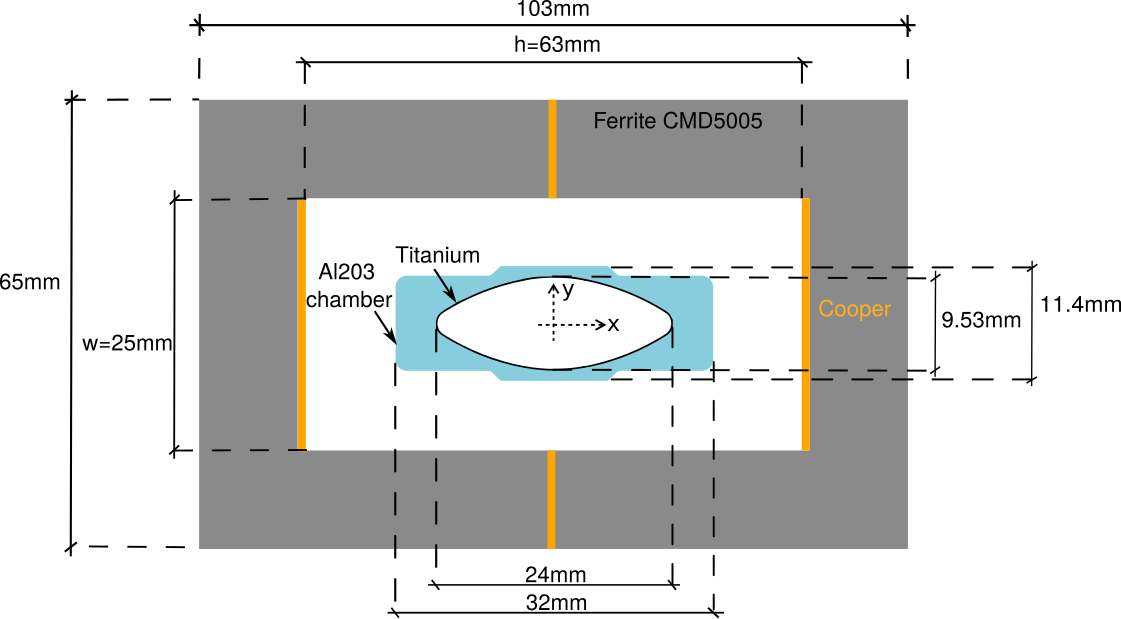
\includegraphics[width=0.8\textwidth]{kicker_magnet.png}
        \caption{Kicker magnet}
        \label{fig:kicker_magnet}
    \end{figure}
    According to the theory~\cite{Nassibian1979,Davino2003}, there are two main contributions to the impedance of this type of magnet: the losses and resonances defined by the materials of the vacuum chamber and the window-frame itself and the coupled flux of the beam with the external circuit that feeds the magnet. While the first contribution dominates the high frequency part of the spectrum, the second is important to the low frequency impedance.

    The coupled flux, first modeled by Nassibian and Sacherer~\cite{Nassibian1979} and improved by Davino and Hahn~\cite{Davino2003} treats the window-frame as a transformer that couples the beam with the external circuit impedance, $Z_g(\omega)$, characterized by the impedance termination of the pulser circuit and the residual capacitances and resistences of the device, which can be accessed via twin wire measurements~\cite{Caspershandbook} of the opened and shorted circuits on the endplates~\cite{Davino2003}. This model predicts impedances for the coupled flux given by
    \begin{align}\label{eq:coupled_flux_impedance}
        Z_\parallel^* = \frac{\Delta^2}{h^2}\frac{i\omega L_2 Z_g}{i\omega L_2 + Z_g},
        \quad Z_X^D = \frac{c}{\omega\Delta^2}Z_\parallel
    \end{align}
    where $\Delta$ is a transverse offset of the beam,
    \begin{align}
        L_2 = \mu_0L\frac{h}{w}\frac{\mu_rt}{\mu_rt+h\funcof{\frac{h}{w}+1}},
    \end{align}
    $L$ is the length of the magnet, $h$ and $w$ are the transverse dimensions defined in Figure~\ref{fig:kicker_magnet}, $t$ is the ferrite thickness and $\mu_r = \mu_r(\omega)$ is the frequency dependent relative magnetic permeability of the ferrite, which can be modeled by
    \begin{align}
        \mu_r(\omega) = \frac{\mu_i-1}{1+i\frac{\omega}{\omega_s}}
    \end{align}
    where $\mu_i$ is the initial permeability and $\omega_s$ is the saturation frequency of the material. Notice in equation~\ref{eq:coupled_flux_impedance} that the coupled flux does not contributes to the vertical impedance and that for a well centered beam, $\Delta=0$ the longitudinal impedance is zero too.

    Considering there is no measurements yet for the circuit impedance, $Z_g(\omega)$, of the kicker magnet, the parametric dependency described in the reference~\cite[eq. 11]{Davino2003}
    \begin{align}
        Z_g(\omega) = \frac{1}{\frac{1}{R_s}+i\omega C_{bb}}
    \end{align}
    was considered for Sirius, where $R_s$ is an equivalent resistance, which was considered \SI{490}{\ohm} in the same reference and $C_{bb}$ is the busbar capacitance, equal to \SI{28.8}{\pico\farad} for their kicker. Figure~\ref{fig:coupled_flux_impedance} shows the coupled flux horizontal impedance for some values of capacitance and resistance, where it is possible to notice the resonant behaviour created by the parallel association of the inductance $L_2$ with the capacitance $C_{bb}$. As this model does not take into account the vacuum chamber, it is expected that higher frequencies will be more damped by the Titanium coating, wich means sources of larger values of capacitance will have small influence on the impedance. For this reason the value considered to model the impedance {\huge to be continued...}

    Regarding the uncoupled flux, there are no formulas in the literature, to the knowledge of the author, to estimate the impedance of an out-of-vacuum window-frame magnet as the one presented in Figure~\ref{fig:kicker_magnet}. There are, however, a model for an in-vacuum magnet developed by Tsutsui in references~\cite{Tsutsui1999,Tsutsui1998,Salvant2010b} that solves \gls{maxeq} exactly for an ultra-relativistic beam, considering the approximate geometry of Figure~\ref{fig:tsutsui_model},
    \begin{figure}[b!]
        \centering
        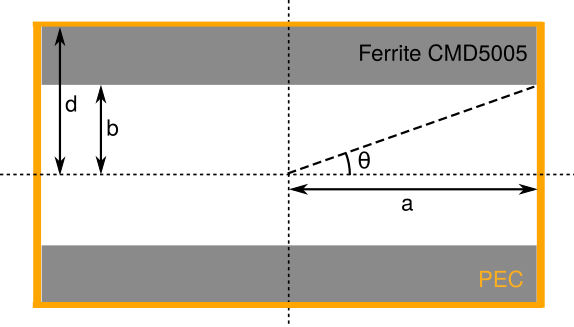
\includegraphics[width=0.5\textwidth]{tsutsui_model.png}
        \caption{Kicker magnet}
        \label{fig:tsutsui_model}
    \end{figure}
    which is infinite in the longitudinal direction. Notice that this model keeps the proportion, $\theta$, of the fields that directly see a very good conductor, in this case approximated by a \gls{pec}, and the lossy material, the ferrite, in relation to the original model.

    In order to estimate the effect of the vacuum chamber on the impedance, other models based on the round multi-layer formulas were developed. These models also tried to account for limiting cases of the Tsutsui geometry in relation to the angle $\theta$ that directly interact with a good conductor. Under this assumptions the models are
    \begin{description}[align=left]
        \item[Worst case:] The angle $\theta$ is zero, which means the beam only sees the ferrite. The layers of the round model in this case are composed by: vacuum, Titanium, ceramic, ferrite and Copper;
        \item[Best case:] The angle $\theta$ is \si{\pi\over2}, which means the beam only sees the good conductor: vacuum, Titanium, ceramic, Copper;
        \item[No Coating:] To evidenciate the effect of the Titanium coating, this layer was removed from the analysis of the worst case model: vacuum, ceramic, ferrite, and Copper.
    \end{description}
    Besides, considering the vacuum chamber is almost an ellipse with high excentricity, the yokoya factors were applied to the round impedace models. Even though this approximation was shown not to work for the low frequency part of the impedance in the tsutsui model~\cite{Salvant2010b}, it is valid for the part of the spectrum dominated by the coating. The impedance of these four models are shown in Figure~\ref{fig:uncoupled_flux_impedance} and the material properties considered in the calculation are shown in table~\ref{tab:material_properties_kicker_impedance}. {\huge to be continued ...}

    For these reasons the

\subsection{Fast Correctors Chambers}

    The Fast orbit correctors of the Sirius storage ring will operate at a update rate of \SI{100}{\kilo\hertz} in the \gls{fofb}~\cite{Tavares2016}, requiring special vacuum chambers in order for such high frequency fields to penetrate. The solution adopted was to brase small and thin stainless steel chambers in the otherwise copper chamber of the ring. The reduced conductance, only \SI{1}{\mega\siemens}, of this material provides a skin depth of \SI{1.6}{\milli\meter} at \SI{100}{\kilo\hertz}, which is much larger than the thickness of the chamber, which is \SI{0.1}{\milli\meter} and do not damp or distort significantly the external field of the magnet.

    The small length of these chambers, only~\SI{10}{\centi\meter}, raises a question on the validity of the infinitely long formulas of the multi-layer chambers used so far. This question is answered by Shobuda and Chin~\cite{Shoduba2009}, who calculate the impedance of a finite resistive insert of finite thickness on a otherwise perfectly conducting and infinitely long round chamber. The authors conclude that even for chambers with length smaller than its radius, with a thickness of the order of \SI{100}{\micro\meter} the impedance of the insert was already equal to the infinitely long chamber counterpart. This results shows that the use of the multi-layer formulas employed so far for the other components are still valid for the fast correctors chambers. Considering this, the relevant parameters used for the modelling of this type of chamber is presented in Table~\ref{tab:fast_correctors_chamber_parameters}.

\subsection{Undulators Chambers}

    For the first phase of operation of the Sirius light source it is predicted the installation of seven \gls{ids} on the storage ring, with four different types of devices: two Delta-type undulators~\cite{DeltaRef} and two \gls{apu}~\cite{APURef}. The design details as well as first experiences with the prototype measuments of the Sirius Delta undulator can be found elsewhere~\cite{SiriusDelta1} and the information regarding the radiation parameters of such devices can be found at~\cite{wikisirius}. All the \gls{ids} will be out of vacuum and their vacuum chamber will be made of copper and coated with \gls{neg}.

    Table~\ref{tab:sirius_undulators} shows the main impedance related parameters of each device type. The close to round shape of the Delta chambers is a good feature, due to the reduced detuning impedance it will generate, which has demonstrated to complicate the operation of machines due to the incoherent tune shift in multibunch configurations~\cite{Nagaoka2001}. Even though the \gls{ids} for the seconde phase of operation are not defined yet, it was extrapolated that all the straight sections available for \gls{id} installation will be filled with the same devices of phase one.

    Figure~\ref{fig:undulators_impedance} shows the vertical dipole and longitudinal wall impedance of the four types of undulators. They were calculated using the parameters of Table~\ref{tab:sirius_undulators}, where the Yokoya factors were applied to the \gls{apu} chambers. These devices will also have quadrupolar impedances that, in this model, will be half of the value of the vertical dipole. Notice the transverse impedance is dominated by the \gls{apu}-19 chamber, while the largest contribution to the longitudinal impedance comes from the Delta-52. This difference comes from the fact that the transverse impedance is more sensitive to the inner radius of the chamber, scaling with $1/r^3$, while the longitudinal impedance goes with $1/r$ and the large length of the Delta-52 compensates for its larger radius.

\section{Geometric Transitions}

    The geometric transitions of the vacuum chamber, also called tapers, are necessary to smoothly change the cross section of the chamber from one geometry to another, in order to avoid discontinuities in the vacuum vessel. In several cases these transitions connect chambers with similar cross sections shapes and different dimensions. When the dimensions of the chamber at the end of the transition is smaller the tapers are called taper-in, and are called taper-out for the opposite case.

    This type of impedance is

\subsection{BC Chamber}
\subsection{RF Cavity taper}
\subsection{Undulators Tapers}

\section{3D-Calculations}
\subsection{BPMs}
\subsection{Bellows}
\subsection{Radiation Masks}

% \section{\Glsentryfull{csr}}
\section{Coherent Synchtrotron Radiation}

\chapter{Impedance Budget}
\section{Longitudinal Impedance}
\subsection{Effective Z/n}
\subsection{Multi-bunch Kloss and Dissipated Power}
\section{Vertical Impedance}
\section{Horizontal Impedance}

\chapter{Simulations and Instabilities Thresholds}
\section{Frequency Domain Calculations}
\subsection{Vertical Plane}
\subsubsection{Single-bunch Tune-Shifts}
\subsubsection{Multi-bunch Tune-Shifts}
\subsubsection{Coupled-Bunch Instabilities}
\subsubsection{Single-Bunch Instabilities}
\subsection{Horizontal Plane}
\subsubsection{Single-bunch Tune-Shifts}
\subsubsection{Multi-bunch Tune-Shifts}
\subsubsection{Coupled-Bunch Instabilities}
\subsubsection{Single-Bunch Instabilities}
\subsection{Longitudinal Plane}
\subsubsection{Multi-Bunch Instabilities}
\subsubsection{Single-Bunch Instabilities}
\section{Time Domain Calculations}
\subsection{Longitudinal Plane}
\subsection{Vertical Plane}
\subsection{Horizontal Plane}


% Finaliza a parte no bookmark do PDF, para que se inicie o bookmark na raiz
\bookmarksetup{startatroot}%

\chapter*[Conclusão]{Conclusão}
\addcontentsline{toc}{chapter}{Conclusão}
\lipsum[1-5]


% --------- Elementos pós-textuais --------------&
\postextual

% Referências bibliográficas
% \bibliographystyle{unsrt}
% \bibliographystyle{numeric}
% \bibliographystyle{plain}
\bibliography{library}
% \printbibliography


% Apêndices
\begin{apendicesenv}
% Imprime uma página indicando o início dos apêndices
\partapendices

\chapter{Lorentz Force Ultra-relativistic limit}\label{app:lorentz_cancel}
    Intuitively, we tend to think the direct interaction between charged particles, such as electric repulsion, is the responsible for the collective effects observed in storage rings, however, as we will see in the subsequent analysis, this is not the main mechanism for ultra-relativistic particles.

    \begin{figure}[hb!]
	    \centering
	    \label{fig:wake1}
	    \begin{tikzpicture}[scale=1]
	        \def\d{1cm}
	        \draw[<->] (1,0) node[below]{$z$}
	        -- ++(-\d,0) node[below left] {$S$}
	        -- ++(0,\d) node[left] {$\rho$}; %coord sys S
	        \draw[<->] (6*\d,0) node[below]{$z'$}
	        -- ++(-\d,0) node[below left] {$S'$}
	        -- ++(0,\d) node[left] {$\rho'$}; % coord sys S'
	        \coordinate (V) at (0.5,0);
	        \coordinate (Q1) at (4cm,1.5cm);
	        \coordinate (Q2) at (0.5cm,2.5cm);
	        \draw[->] (5*\d,0.5*\d) -- ++(V) node[above] {$\boldsymbol{v}$};
	        \filldraw[fill=black] (Q1) circle[radius=0.05] node[above] {$q$}; % source particle
	        \draw[->] (Q1) -- ++(V) node[above] {$\boldsymbol{v}$}; % velocity vector
	        \filldraw[fill=black] (Q2)  circle[radius=0.05]; % test particle
	        \draw[->] (Q2) -- ++(V) node[above] {$\boldsymbol{v}$}; % velocity vector
	        \draw[dashed,|-|] ($(Q1)-(0,0.2)$)
	        let \p1 = ($(Q2) - (Q1)$)
	        in -- ++(\x1,0) node[midway,below] {$s$}; %horizontal distance
	        \draw[dashed,|-|] ($(Q2)-(0.2,0)$)
	        let \p1 = ($(Q1) - (Q2)$)
	        in -- ++(0,\y1) node[midway,left] {$\rho$}; % vertical distance
	        \draw[->] (Q1) -- ++($(Q2) - (Q1)$) node[midway,above] {$\boldsymbol{R}$}; %vector
	    \end{tikzpicture}
	    \caption{Duas partículas interagindo via campo direto.}
    \end{figure}

    To see this lets consider the interaction of a source particle $Q$ moving with velocity $\vect{v}=v{\vect{\hat{z}}}$ with a witness particle $q$ moving with the same velocity (parallel path) at a distance $s$ in the direction parallel to the movement and at a transverse distance $\rho$, as shown in Figure\,\ref{fig:wake1}. We want to determine the force that the source particle exerts on the witness particle. One way to do this is by calculating the electric field of the source particle in the co-moving frame of reference, $S'$, and Lorentz transforming it back to the laboratory's frame. After the math we obtain:

    \begin{align}\label{eq:fields_free_particle}
    	\vect{E} = \frac{q}{4\pi\epsilon_0}\frac{\vect{R}}{\gamma^2 R^{*3}}, & & \vect{B} = \frac{1}{c^2}\vect{v} \times \vect{E}
    \end{align}
    where $\vect{R}$ is the vector which connects both particles, going from the source to the witness and  $R^{*2} = s^2 + x^2/\gamma^2$, e $\gamma = 1/(1-v^2/c^2)$.

    Combining equation\,\ref{eq:fields_free_particle} with the Lorentz force, we get the longitudinal and transverse force over the witness particle:
    \begin{align}\label{eq:space_charge_force}
    	F_l &= E_z = -\frac{q}{4\pi\epsilon_0}\frac{s}{\gamma^2\left(s^2+x^2/\gamma^2\right)^{3/2}}, \\
    	F_t &= E_x - vB_y = -\frac{q}{4\pi\epsilon_0}\frac{x}{\gamma^4\left(s^2+x^2/\gamma^2\right)^{3/2}}
    \end{align}

    In accelerator physics the force $\vect{F}$ is known as space charge force. We can infer from equation\,\ref{eq:space_charge_force} that for any position $s$ and $x$, the longitudinal force is proportional to $\gamma^{-2}$ and $F_t \sim \gamma^{-4}$ if $s \gg x/\gamma$ and  $F_t \sim \gamma^{-1}$ if $s \approx 0$. This way, in the ultra-relativistic limit, $\gamma \to \infty$, the electromagnetic interaction between particles moving parallel to each other in free space is zero. It is easy to show that in this limit, if the movement of the particles is not parallel, there is an interaction force only for $s=0$, but, as their speed is the same, this situation can only happen for an infinitesimal time.

    In this work we are interested in the the interaction between particles in the ultra-relativistic limit, $v \to c$. The space charge effects discussed above are despicable in this limit and the interaction between the particles is due to the presence of the walls of the vacuum chamber. Note that taking the limit $v \to c$ in the equation\,\ref{eq:fields_free_particle} and remembering that $s = vt - z$, we can write the electromagnetic field of a ultra-relativistic charge as
    \begin{align}
    	\vect{E} =
		\frac{q}{2\pi\epsilon_0}\frac{\vect{\hat{r}}}{r}\delta(z-ct), &
		& \vect{B} =\frac{1}{c}\vect{\hat{z}}\times\vect{E},
    \end{align}
    where $\vect{r} = \vect{\hat{x}}x + \vect{\hat{y}}y$ is a bidimensional vector in cylindrical coordinates ($\vect{\hat{x}}$ and $\vect{\hat{y}}$ are unit vectors in the $x$ e $y$ directions, respectively). The equations above show that the field is pancake-like and follow the beam as it travels through the empty space. It is important to notice that this solution is steady-state, it was necessary an infinite amount of time before $t$ to build it and that's why there is no causal paradoxes in it.

    \begin{figure}[hb!]
	    \centering
	    \label{fig:wake2}
	    \begin{tikzpicture}
	        \draw[very thick] (0,0) -- ++(10,0) (0,4) -- ++(10,0); %vacuum chamber
	        \draw[dashed] (0,2) -- ++(10,0); %eixo de simetria
	        \coordinate (V) at (0.5,0);
	        \coordinate (Q1) at (4cm,2.2cm);
	        \coordinate (Q2) at (0.5cm,2.5cm);
	        \filldraw[fill=black] (Q1) circle[radius=0.05] node[left] {$q$}; % source particle
	        \draw[->] (Q1) -- ++(V) node[above] {$\boldsymbol{v}$}; % velocity vector
	        \draw[-{Stealth[length=10pt]}] (Q1) let \p1 = (Q1) in --(\x1,4);
	        \draw[-{Stealth[length=10pt]}] (Q1) let \p1 = (Q1) in --(\x1,0) node[midway,right] {$\boldsymbol{E}$};
	        \draw ($(Q1)+(0,1)$) circle[radius=0.2] node[right=0.2] {$\boldsymbol{B}$};
	        \filldraw ($(Q1)+(0,1)$) circle[radius=0.07];
	    \end{tikzpicture}
	    \caption{Particles interacting in a perfectly conducting cylindrical tube.}
    \end{figure}

    Lets consider now a pipe with cylindrical symmetry\footnote{do not confuse cylindrical symmetry with cylinder. By cylindrical symmetry we mean a system with translational symmetry in one direction.}, hollow and with absolute vacuum in its interior, made of a perfect electric conductor material and with arbitrary cross section. If we put the particles of the previous example inside this pipe, moving parallel to symmetry axis, they will induce image charges in the surface of the wall which cancel the electromagnetic field inside the metal.

    The image charges travel with the same velocity $\vect{v}$ of the particles (see Figure\,\ref{fig:wake2}). As they move in parallel paths with constant velocity, in the limit $v \to c$, according to the previous results, they do not interact, independently of how close they are from each other.

    From this analysis we conclude that the interaction between particles in the ultra-relativistic limit can occur only for two reasons:
    \begin{itemize}
    \item The wall is not perfectly conducting, or
    \item The pipe does not have cylindrical symmetry (which generally is due to the presence of RF cavities, flanges, bellows, beam position monitors, vacuum pumps, among other elements in the vacuum chamber of an accelerator).
    \end{itemize}


\chapter{Duas partículas interagindo no vácuo}

    \begin{figure}[hb!]
	    \centering
	    \begin{tikzpicture}[scale=1]
		    \def\d{1cm}
		    \draw[<->] (1,0) node[below]{$z$}
				-- ++(-\d,0) node[below left] {$S$}
		        -- ++(0,\d) node[left] {$\rho$}; %coord sys S
		    \draw[<->] (6*\d,0) node[below]{$z'$}
				-- ++(-\d,0) node[below left] {$S'$}
		        -- ++(0,\d) node[left] {$\rho'$}; % coord sys S'
		    \coordinate (V) at (0.5,0);
		    \coordinate (Q1) at (4cm,1.5cm);
		    \coordinate (Q2) at (0.5cm,2.5cm);
		    \draw[->] (5*\d,0.5*\d) -- ++(V) node[above] {$\boldsymbol{v}$};
		    \filldraw[fill=black] (Q1) circle[radius=0.05] node[above] {$q$}; % source particle
		    \draw[->] (Q1) -- ++(V) node[above] {$\boldsymbol{v}$}; % velocity vector
		    \filldraw[fill=black] (Q2)  circle[radius=0.05]; % test particle
		    \draw[->] (Q2) -- ++(V) node[above] {$\boldsymbol{v}$}; % velocity vector
		    \draw[dashed,|-|] ($(Q1)-(0,0.2)$)
						   let \p1 = ($(Q2) - (Q1)$)
		                   in -- ++(\x1,0) node[midway,below] {$s$}; %horizontal distance
		    \draw[dashed,|-|] ($(Q2)-(0.2,0)$)
						   let \p1 = ($(Q1) - (Q2)$)
		                   in -- ++(0,\y1) node[midway,left] {$\rho$}; % vertical distance
		    \draw[->] (Q1) -- ++($(Q2) - (Q1)$) node[midway,above] {$\boldsymbol{R}$}; %vector
	    \end{tikzpicture}
	    \caption{Duas partículas interagindo via campo direto.}
    \end{figure}

    Primeiro, campos gerados por $q_1$. No referencial $S'$:
    \begin{align}
		\vect{E'} &= \frac{q}{4\pi\epsilon_0} \frac{\vect{\hat{r'}}}{r'^2} \\
		\vect{B'} &= \vect{0'}
    \end{align}
    assumindo que a partícula 1 está na origem do sistema de coordenadas $S'$.

    Lembrando que a transformação entre coordenadas esféricas para cilíndricas são:
    \begin{align}
		r' &= \sqrt{s'^2 + \rho'^2} \\
		\vect{\hat{r'}} &= \cos\theta'\vect{\hat{z'}} +
	 				   	   \sin\theta'\vect{\hat{\rho'}} =
    	-\frac{s'}{r'}\vect{\hat{z'}} + \frac{\rho'}{r'}\vect{\hat{\rho'}}
    \end{align}
    onde a coordenada $\phi$ fica inalterada.

    Assim podemos reescrever o campo elétrico em suas partes longitudinal e transversal:
    \begin{align}
		\vect{E'}_{||} &= \frac{q}{4\pi\epsilon_0} \frac{\cos\theta'\vect{\hat{z'}}}{r'^2} =
                 	-\frac{q}{4\pi\epsilon_0} \frac{s'\vect{\hat{z'}}}{(\rho'^2+s'^2)^{3/2}} \\
		\vect{E'}_{\perp} &= \frac{q}{4\pi\epsilon_0} \frac{\sin\theta'\vect{\hat{\rho'}}}{r'^2} =
                     \frac{q}{4\pi\epsilon_0} \frac{x'\vect{\hat{\rho'}}}{(\rho'^2+s'^2)^{3/2}}
    \end{align}

    Lembrando as equações de transformação de Lorentz para campos elétricos e magnéticos, para esse problema:

    \begin{align}
 		\vect{E}_{||} &= \vect{E'}_{||}\\
 		\vect{B}_{||} &= \vect{B'}_{||}\\
 		\vect{E}_\perp &= \gamma\left(\vect{E'}_\perp - \vect{v}\times\vect{B'}\right)\\
 		\vect{B}_\perp &= \gamma\left(\vect{B'}_\perp + \frac{1}{c^2}\vect{v}\times\vect{E'}\right)
    \end{align}

    Ainda, as coordenadas espaciais são transformadas da seguinte maneira:

    \begin{align}
		\vect{\hat{\rho}} &=\vect{\hat{\rho'}}, \quad \vect{\hat{z}} = \vect{\hat{z'}}\\
		\rho &= \rho', \quad z = \frac{z'}{\gamma}
    \end{align}

    Assim, podemos notar que:

    \begin{align}
		\vect{E}_{||} &= -\frac{q}{4\pi\epsilon_0} \frac{s'\vect{\hat{z'}}}{(\rho'^2+s'^2)^{3/2}} =
				 -\frac{q}{4\pi\epsilon_0} \frac{\gamma s\vect{\hat{z}}}{((\gamma s)^2+\rho^2)^{3/2}}=
                 -\frac{q}{4\pi\epsilon_0} \frac{s\vect{\hat{z}}}{\gamma^2R^{*3}} \\
		\vect{E}_\perp&= \frac{q}{4\pi\epsilon_0}\frac{\gamma \rho'\vect{\hat{\rho'}}}{(\rho'^2+s'^2)^{3/2}} =
				 \frac{q}{4\pi\epsilon_0}\frac{\gamma \rho\vect{\hat{\rho}}}{((\gamma s)^2+\rho^2)^{3/2}}=
                 \frac{q}{4\pi\epsilon_0} \frac{\rho\vect{\hat{\rho}}}{\gamma^2R^{*3}} \\
		\vect{B}_\perp&= -\frac{\gamma   vE'_\perp}{c^2}\vect{\hat{\phi'}} =
		         -\frac{vE_\perp}{c^2}\vect{\hat{\phi}}
    \end{align}
    onde $R^* = \sqrt{s^2+\left(\rho/\gamma\right)^2}$

    Agora podemos analisar a força exercida pela partícula fonte sobre a partícula teste usando a força de Lorentz
    \begin{equation}
    	\vect{F} = \left(\vect{E} + \vect{v}\times\vect{B}\right)
    \end{equation}
    onde foi assumida carga unitária para a partícula teste, e os campos calculados anteriormente.

    Assumindo que a velocidade da partícula teste é a mesma da partícula fonte (mesmo módulo e direção), as componentes longitudinal e transversal da força ficam:

    \begin{align}
		\vect{F}_{||} &= \vect{E}_{||} = -\frac{q}{4\pi\epsilon_0} \frac{s\vect{\hat{z}}}{\gamma^2R^{*3}}\\
		\vect{F}_\perp&= \left(1+\frac{\vect{v}\times\vect{v}\times}{c^2}\right)\vect{E}_\perp =
                 \left(1-\frac{v^2}{c^2}\right)\vect{E}_\perp =
                 \frac{q}{4\pi\epsilon_0} \frac{\rho\vect{\hat{z}}}{\gamma^4R^{*3}}
    \end{align}
    onde vemos que a força longitudinal tende a zero proporcionalmente a $\gamma^{-2}$ quando $v \to c$ e que a força longitudinal tende a zero com $\gamma^{-4}$, se $s>\rho/\gamma$ e com $\gamma^{-1}$ se $s<\rho/\gamma$.

    Agora, vamos assumir que a velocidade da partícula teste não é paralela à velocidade da partícula fonte
    \begin{equation}
    	\vect{v_2} = v(\cos\delta \vect{\hat{z}} + \sin\delta\vect{\hat{\rho}})
    \end{equation}

    Assim, a força sofrida por essa partícula fica

    \begin{equation}\begin{aligned}
    	\vect{F} &= \vect{E}_{||} + \vect{E}_\perp - v(\cos\delta \vect{\hat{z}} + \sin\delta\vect{\hat{\rho}}) \times \vect{\hat{\phi}}\frac{vE_\perp}{c^2} \\
		&= \left(1-\frac{v^2}{c^2}\cos\delta\right)\vect{E}_\perp + \vect{E}_{||} + \frac{v^2}{c^2}E_\perp\sin\delta\vect{\hat{z}}
    \end{aligned}\end{equation}

    Olhando essa expressão, vemos que, conforme $v \to c$, a força pode ser expressa como:

    \begin{equation}
    	\vect{F} = \left\{
    	\begin{aligned}
    		\left((1-\cos\delta)\vect{\hat{\rho}} + \sin\delta\vect{\hat{z}}\right)
    		\frac{q}{4\pi\epsilon_0} \frac{\gamma\vect{\hat{\rho}}}{\rho^2} & &|s|<\rho/\gamma\\
    		0 & &|s|>\rho/\gamma
    	\end{aligned}\right.
    \end{equation}


\chapter{Causality and catch up distance}\label{app:causality}

    If one particle moves in a straight line at light speed, the electromagnetic field scattered by the discontinuities of the chamber will not catch up with it and will not affect the charges travelling ahead of it. The field will only interact with the charges moving behind of the source particle. Such property is known as causality.

    Even though this property is not strictly true in the real world, because particles always travel at speeds lower than the light's, it is true in most practical cases, as we will see bellow.

    Lets try to calculate the distance $z$ where the field generated by some discontinuity in the vacuum chamber will catch up with a witness particle at a distance $s$ behind the source particle. At the time $t=0$ the source particle passes through the discontinuity and an electromagnetic wave is generated with its wave front travelling at the speed of light in all directions, forming a sphere of radius $R$, see FigureXX. At any given time after this, the following relation holds:
    \begin{align}
		ct = R \quad vt = z && \Rightarrow && R = \frac{z}{\beta} \quad \text{where} \,\, \beta = \frac{v}{c}
    \end{align}
    where $z$ is the distance travelled by the source particle. Besides that, at the specific time when the wake catchs up with the witness particle, the following relation is valid:
    \begin{align}
		R^2 = b^2 + (z-s)^2  \Rightarrow z^2(\frac{1}{\beta^2}-1) + 2sz - (b^2 + s^2) = 0  \Rightarrow \\
		z = -\gamma^2 \beta^2 s + \sqrt{s^2\gamma^4\beta^4 + \gamma^2\beta^2\left(b^2 + s^2\right)}  = \gamma^2 \beta^2 s\left(-1 + \sqrt{1 + \frac{1}{\gamma^2\beta^2}\left(1 + \frac{b^2}{s^2}\right)}\right)
    \end{align}
    where $b$ is the distance from the discontinuity to the trajectory of the particles and $\gamma = 1/\sqrt{1-\beta^2}$ is the relativistic energy. FigureXX shows a graphic of this function, normalized by the distance $b$. We notice that, for $s=0$, which means the field catching up with the source particle, $z = \gamma\beta b$. For the case of Sirius, $\gamma \approx 5870$ and $\beta \approx 1$, if $ b = 2$mm, $z \approx 12$m.

    \begin{figure}[hb!]
	    \centering
	    \label{fig:catch_up}
	    \begin{tikzpicture}
	    \draw[very thick] (0,0) -- ++(10,0) (0,4) -- ++(10,0); %vacuum chamber
	    \draw[very thick] (4.8,4) to [out=-90,in=0] (5,3.8) to [out=180,in=-90] (5.2,4);
	    \draw[dashed] (0,2) -- ++(10,0); %eixo de simetria
	    \coordinate (V) at (0.5,0);
	    \coordinate (Q1) at (4cm,2.2cm);
	    \coordinate (Q2) at (0.5cm,2.5cm);
	    \filldraw[fill=black] (Q1) circle[radius=0.05] node[left] {$q$}; % source particle
	    \draw[->] (Q1) -- ++(V) node[above] {$\boldsymbol{v}$}; % velocity vector
	    \draw[-{Stealth[length=10pt]}] (Q1) let \p1 = (Q1) in --(\x1,4);
	    \draw[-{Stealth[length=10pt]}] (Q1) let \p1 = (Q1) in --(\x1,0) node[midway,right] {$\boldsymbol{E}$};
	    \draw ($(Q1)+(0,1)$) circle[radius=0.2] node[right=0.2] {$\boldsymbol{B}$};
	    \filldraw ($(Q1)+(0,1)$) circle[radius=0.07];
	    \end{tikzpicture}
	    \caption{The catch up distance.}
    \end{figure}


    \chapter{Check Panofsky-Wenzel}\label{app:check_panofky}

    As the velocity of the particle is in the longitudinal direction we have
    \begin{align}
    	\dertot{a}{t} = \derpar{a}{t} + v\derpar{a}{s}
    \end{align}
    where $a$ can be any of the components of vector potential or the scalar potential. This way, since all fields and potentials go to zero in infinity, we always have this equality for the integral of these quantities:
    \begin{align}
    	\infint{t}{\left(\derpar{a}{t} + v\derpar{a}{s}\right)|_{s=vt-z}} = 0.
    \end{align}
    Besides, since the integration in time happens with $s=vt-z$, we have
    \begin{align}
    	\derpar{}{z}\left(\infint{t}{a}\right) =
    	\infint{t}{\derpar{a}{s}\derpar{s}{z}} =
    	-\infint{t}{\derpar{a}{s}}
    \end{align}
    Also, lets remember the relations between the electromagnetic fields and the potentials:
    \begin{align}
    	E_x &= -\derpar{A_x}{t} - \derpar{\phi}{x} &
        	& B_x = \derpar{A_y}{s} - \derpar{A_s}{y}\\
    	E_y &= -\derpar{A_y}{t} - \derpar{\phi}{y} &
        	& B_y = \derpar{A_s}{x} - \derpar{A_x}{s}\\
    	E_s &= -\derpar{A_s}{t} - \derpar{\phi}{s} &
        	& B_s = \derpar{A_x}{y} - \derpar{A_y}{x}
    \end{align}
    \begin{align}
    	w_s = \derpar{W}{z}\nonumber
    	&= \frac{c}{qQ} \derpar{}{z}\left(\infint{t}{\left(vA_s-\phi\right)}\right)
    	= \frac{c}{qQ} \infint{t}{\left(-v\derpar{A_s}{s}+\derpar{\phi}{s}\right)}\\
    	&= \frac{c}{qQ} \infint{t}{\left(\derpar{A_s}{t}+\derpar{\phi}{s}\right)}
    	=-\frac{c}{qQ} \infint{t}{E_s}\\[1cm]
    	w_x = \derpar{W}{x}\nonumber
    	&=\frac{c}{qQ} \infint{t}{\left(v\derpar{A_s}{x}-\derpar{\phi}{x}\right)}\\
    	&= \frac{c}{qQ} \infint{t}{\left(vB_y+v\derpar{A_x}{s} + E_x + \derpar{A_x}{t}\right)}
    	= \frac{c}{qQ} \infint{t}{\left(E_x + vB_y\right)}\\[1cm]
    	w_y = \derpar{W}{y}\nonumber
    	&=\frac{c}{qQ} \infint{t}{\left(v\derpar{A_s}{y}-\derpar{\phi}{y}\right)}\\
    	&=\frac{c}{qQ} \infint{t}{\left(-vB_x+v\derpar{A_y}{s} + E_y + \derpar{A_y}{t}\right)}
    	= \frac{c}{qQ} \infint{t}{\left(E_y + vB_x\right)}
    \end{align}


\chapter{Symmetry analysis}\label{app:symmetry_analysis}

    First lets consider the general expansion of the Wake potential of a bunch in the transverse coordinates of the centroid of the source $(x_s,y_s)$ and the integration path $(x,y)$ up to third order:

    \begin{align}
		W(\vect{x},s) &= W_0(s) + \sum_{i=1}^4 M_i(s) x_i + \frac12\sum_{i,j=1}^4 D_{ij}(s) x_i x_j + \frac13\sum_{i,j,k=1}^4 Q_{ijk}(s) x_i x_j x_k
    \end{align}
    where we considered $\vect{x} = (x_1,x_2,x_3,x_4) = (x_s,y_s,x,y)$ and because of the commutative property of multiplication, we can set $D_{ij} = D_{ji}$ and $Q_{ijk}=Q_{kij}=Q_{jki}=Q_{ikj}=Q_{jik}=Q_{kji}$ without loss of generality. With these considerations, number of independent components of $D$ is 10 and $Q$ is 20. Besides that, the fact that $W$ is an harmonic function of the transverse coordinates of the integration path, imposes that
    \begin{align}
		D_{33} &= - D_{44} \\
		Q_{33i} &= - Q_{44i}, \quad \text{with} \quad i=1,2,3,4
    \end{align}
    which leaves only nine independent components of $D$ and sixteen of $Q$.

    Thus, the wake forces become:
    \begin{align}
		F_L(\vec{x},s) = W'(\vec{x},s) &= W_0' + \sum_{i=1}^4 M_i' x_i + \frac12\sum_{i,j=1}^4 D_{ij}' x_i x_j + \frac13\sum_{i,j,k=1}^4 Q_{ijk}' x_i x_j x_k \\
		F_x(\vec{x},s) = \derpar{W(\vect{x},s)}{x} &= M_3 + \sum_{i=1}^4 D_{3i} x_i + \sum_{i,j=1}^4 Q_{3ij} x_i x_j \\
		F_y(\vec{x},s) = \derpar{W(\vect{x},s)}{y} &= M_4 + \sum_{i=1}^4 D_{4i} x_i + \sum_{i,j=1}^4 Q_{4ij} x_i x_j
    \end{align}

    Generally we are interested in obtaining the linear terms as function of the transverse coordinates correct up to second order. It means we want to isolate the linear from the quadract terms in the simulations. Thus, lets keep only the second order terms in the wake forces above.
    \begin{align}
		F_L(\vect{x},s) &= W_0' + \vect{M'}^T \cdot \vect{x} + \frac12\vect{x}^T \cdot \tensor{D'}  \cdot \vect{x} \\
		F_x(\vect{x},s) &= M_x + \vect{D_x}^T \cdot \vect{x} +        \vect{x}^T \cdot \tensor{Q_x} \cdot \vect{x} \\
		F_y(\vect{x},s) &= M_y + \vect{D_y}^T \cdot \vect{x} +        \vect{x}^T \cdot \tensor{Q_y} \cdot \vect{x}
    \end{align}
    where
    \begin{align}
		\vect{M} &= \begin{pmatrix*}[r] M_{1}\\ M_{2}\\ M_{3}\\ M_{4}\end{pmatrix*} \\
		\tensor{D}  &= \begin{pmatrix*}[r] D_{11} & D_{12} & D_{13} & D_{14} \\
                                   D_{21} & D_{22} & D_{23} & D_{24} \\
                                   D_{31} & D_{32} & D_{33} & D_{34} \\
                                   D_{41} & D_{42} & D_{43} & D_{44}
               \end{pmatrix*} =
               \begin{pmatrix*}[r] D_{11} & D_{12} & D_{13} & D_{14} \\
                                   D_{12} & D_{22} & D_{23} & D_{24} \\
                                   D_{13} & D_{23} & D_{33} & D_{34} \\
                                   D_{14} & D_{24} & D_{34} & -D_{33}
               \end{pmatrix*}\\
		\vect{D_x} &= \tensor{D}\cdot \vect{\hat{x}} \\
		\vect{D_y} &= \tensor{D}\cdot \vect{\hat{y}} \\
		\tensor{Q_x}&= \begin{pmatrix*}[r] Q_{311} & Q_{312} & Q_{313} & Q_{314} \\
                                   Q_{321} & Q_{322} & Q_{323} & Q_{324} \\
                                   Q_{331} & Q_{332} & Q_{333} & Q_{334} \\
                                   Q_{341} & Q_{342} & Q_{343} & Q_{344}
               \end{pmatrix*} =
               \begin{pmatrix*}[r] Q_{113} & Q_{123} & Q_{133} & Q_{134} \\
                                   Q_{123} & Q_{223} & Q_{233} & Q_{234} \\
                                   Q_{133} & Q_{233} & Q_{333} & Q_{334} \\
                                   Q_{134} & Q_{234} & Q_{334} & -Q_{333}
               \end{pmatrix*}\\
		\tensor{Q_y}&= \begin{pmatrix*}[r] Q_{411} & Q_{412} & Q_{413} & Q_{414} \\
                                   Q_{421} & Q_{422} & Q_{423} & Q_{424} \\
                                   Q_{431} & Q_{432} & Q_{433} & Q_{434} \\
                                   Q_{441} & Q_{442} & Q_{443} & Q_{444}
               \end{pmatrix*} =
               \begin{pmatrix*}[r] Q_{114} & Q_{124} & Q_{134} & Q_{133} \\
                                   Q_{124} & Q_{224} & Q_{234} & Q_{233} \\
                                   Q_{134} & Q_{234} & Q_{334} & -Q_{333} \\
                                   Q_{133} & Q_{233} &-Q_{333} & -Q_{334}
               \end{pmatrix*}\\
    \end{align}



    Due to their importance, some components of the $D$ tensor have a name: the $D_{31}$ and $D_{42}$ are called dipolar wakes; and $D_{33}$ and $D_{44}$ are the quadrupolar wakes. While the first generates coherent tune-shifts and instabilities, the later is the responsible for incoherent tune-shifts of the beam. The other terms are the skew components, which are zero for most practical cases, as we will see below.

    When the geometry has symmetry the number of independent compononts in $M$, $D$ and $Q$ are reduced even more.
    When the symmetry occurs in one plane, the number of independent components is two, five and eight, respectivelly.Below we list examples for the most practical cases:

    \begin{itemize}
    \item symmetry in the $yz$ plane, or $x=0$.
    \begin{align}
		W(x_s,y_s,x,y,s) = & W(-x_s,y_s,-x,y,s) \Rightarrow \\
		M_2= & M_4=0\\
		D_{12}=D_{14}= & D_{23}=D_{34}=0\\
		Q_{111}=Q_{122}= & Q_{113}=Q_{223}=0\\
		Q_{133}=Q_{333}= & Q_{124}=Q_{234}=0
    \end{align}
    \begin{align}
		\vect{M}&= \begin{pmatrix} M_{1}\\ 0\\ M_{3}\\ 0\end{pmatrix} &
		\tensor{D} &= \begin{pmatrix} D_{11} &    0   & D_{13} &    0    \\
                                  0   & D_{22} &    0   &  D_{24} \\
                               D_{13} &    0   & D_{33} &    0    \\
                                  0   & D_{24} &    0   & -D_{33}
               \end{pmatrix}\\
		\tensor{Q_x}&=\begin{pmatrix}    0    & Q_{123} &    0    & Q_{134} \\
                               Q_{123} &    0    & Q_{233} &    0    \\
                                  0    & Q_{233} &    0    & Q_{334} \\
                               Q_{134} &    0    & Q_{334} &    0
               \end{pmatrix} &
		\tensor{Q_y}&=\begin{pmatrix} Q_{114} &    0    & Q_{134} &    0    \\
                                  0    & Q_{224} &    0    & Q_{233} \\
                               Q_{134} &    0    & Q_{334} &    0    \\
                                  0    & Q_{233} &    0    & -Q_{334}
               \end{pmatrix}
    \end{align}

    \item symmetry in the $xz$ plane, or $y=0$.
    \begin{align}
		W(x_s,y_s,x,y,s) = & W(x_s,-y_s,x,-y,s) \Rightarrow \\
		M_1= & M_3=0\\
		D_{12}=D_{14}= & D_{23}=D_{34}=0\\
		Q_{112}=Q_{222}= & Q_{123}=Q_{233}=0\\
		Q_{114}=Q_{224}= & Q_{134}=Q_{334}=0
    \end{align}
    \begin{align}
		\vect{M}    &= \begin{pmatrix}   0  \\ M_{2}\\  0  \\ M_{4}\end{pmatrix} &
		\tensor{D}  &= \begin{pmatrix} D_{11} &    0   & D_{13} &    0   \\
                                  0   & D_{22} &    0   & D_{24} \\
                               D_{13} &    0   & D_{33} &    0   \\
                                  0   & D_{24} &    0   & -D_{33}
               \end{pmatrix}\\
		\tensor{Q_x}&= \begin{pmatrix} Q_{113} &    0    & Q_{133} &    0    \\
                                  0    & Q_{223} &    0    & Q_{234} \\
                               Q_{133} &    0    & Q_{333} &    0    \\
                                  0    & Q_{234} &    0    & -Q_{333}
               \end{pmatrix} &
		\tensor{Q_y}&= \begin{pmatrix}    0    & Q_{124} &    0    & Q_{133} \\
                               Q_{124} &    0    & Q_{234} &    0    \\
                                  0    & Q_{234} &    0    & -Q_{333} \\
                               Q_{133} &    0    &-Q_{333} &    0
               \end{pmatrix}
    \end{align}

    \item symmetry in the plane $y=x$.
    \begin{align}
		W(x_s,y_s,x,y,s) =& W(y_s,x_s,y,x,s) \Rightarrow \\
		M_1=M_2, \quad & M_3=M_4\\
		D_{11}=D_{22}, \quad D_{13}=D_{24}, \quad & D_{14}=D_{23}, \quad D_{33}=0 \\
		Q_{111}=Q_{222}, \quad Q_{112}= Q_{122}, \quad & Q_{113}=Q_{224}, \quad Q_{114}= Q_{223} \\
		Q_{123}=Q_{124}, \quad Q_{133}=-Q_{233}, \quad & Q_{134}=Q_{234}, \quad Q_{333}=-Q_{334}
    \end{align}
    \begin{align}
		\vect{M}  &= \begin{pmatrix} M_{1}\\ M_{1}\\ M_{3}\\ M_{3}\end{pmatrix} &
		\tensor{D}   &=\begin{pmatrix} D_{11} & D_{12} & D_{13} & D_{14} \\
                               D_{12} & D_{11} & D_{14} & D_{13} \\
                               D_{13} & D_{14} &    0   & D_{34} \\
                               D_{14} & D_{13} & D_{34} &    0
               \end{pmatrix}\\
		\tensor{Q_x}&= \begin{pmatrix} Q_{113} & Q_{123} & Q_{133} & Q_{134} \\
                               Q_{123} & Q_{114} &-Q_{133} & Q_{134} \\
                               Q_{133} &-Q_{133} & Q_{333} &-Q_{333} \\
                               Q_{134} & Q_{134} &-Q_{333} &-Q_{333}
               \end{pmatrix} &
		\tensor{Q_y} &=\begin{pmatrix} Q_{114} & Q_{123} & Q_{134} & Q_{133} \\
                               Q_{123} & Q_{113} & Q_{134} &-Q_{133} \\
                               Q_{134} & Q_{134} &-Q_{333} &-Q_{333} \\
                               Q_{133} &-Q_{133} &-Q_{333} & Q_{333}
               \end{pmatrix}
    \end{align}

    \item symmetry in the plane $y=-x$.
    \begin{align}
		W(x_s,y_s,x,y,s) =& W(-y_s,-x_s,-y,-x,s) \Rightarrow \\
		M_1=-M_2, \quad & M_3=-M_4\\
		D_{11}=D_{22}, \quad D_{13}=D_{24}, \quad & D_{14}=D_{23}, \quad D_{33}=0 \\
		Q_{111}=-Q_{222}, \quad Q_{112}=-Q_{122}, \quad & Q_{113}=-Q_{224}, \quad Q_{114}=-Q_{223} \\
		Q_{123}=-Q_{124}, \quad Q_{133}= Q_{233}, \quad & Q_{134}=-Q_{234}, \quad Q_{333}= Q_{334}
    \end{align}
    \begin{align}
		\vect{M}  &= \begin{pmatrix} M_{1}\\ -M_{1}\\ M_{3}\\ -M_{3}\end{pmatrix} &
		\tensor{D}   &=\begin{pmatrix} D_{11} & D_{12} & D_{13} & D_{14} \\
                               D_{12} & D_{11} & D_{14} & D_{13} \\
                               D_{13} & D_{14} &    0   & D_{34} \\
                               D_{14} & D_{13} & D_{34} &    0
               \end{pmatrix}\\
		\tensor{Q_x}&= \begin{pmatrix} Q_{113} & Q_{123} & Q_{133} & Q_{134} \\
                               Q_{123} &-Q_{114} & Q_{133} &-Q_{134} \\
                               Q_{133} & Q_{133} & Q_{333} & Q_{333} \\
                               Q_{134} &-Q_{134} & Q_{333} &-Q_{333}
               \end{pmatrix} &
		\tensor{Q_y} &=\begin{pmatrix} Q_{114} &-Q_{123} & Q_{134} & Q_{133} \\
                              -Q_{123} &-Q_{113} &-Q_{134} & Q_{133} \\
                               Q_{134} &-Q_{134} & Q_{333} &-Q_{333} \\
                               Q_{133} & Q_{133} &-Q_{333} &-Q_{333}
               \end{pmatrix}
    \end{align}
    \end{itemize}

    Below we combine some of the above mentioned symmetries which are very common in the simulations performed for accelerators elements:

    \begin{itemize}
    \item x=0 and y=0.
    \begin{align}
		\vect{M}= \vect{0} & &
		\tensor{D} = \begin{pmatrix} D_{11} &    0   & D_{13} &    0    \\
                                  0   & D_{22} &    0   &  D_{24} \\
                               D_{13} &    0   & D_{33} &    0    \\
                                  0   & D_{24} &    0   & -D_{33}
               \end{pmatrix} & &
		\tensor{Q_x}=\tensor{0} & &
		\tensor{Q_y}=\tensor{0}
    \end{align}

    \item $y=-x$ and $y=x$.
    \begin{align}
		\vect{M}= \vect{0} & &
		\tensor{D}   &=\begin{pmatrix} D_{11} & D_{12} & D_{13} & D_{14} \\
                               D_{12} & D_{11} & D_{14} & D_{13} \\
                               D_{13} & D_{14} &    0   & D_{34} \\
                               D_{14} & D_{13} & D_{34} &    0
               \end{pmatrix}& &
		\tensor{Q_x}=\tensor{0} & &
		\tensor{Q_y}=\tensor{0}
    \end{align}

    \item $x=0$, $y=0$, $y=-x$ and $y=x$.
    \begin{align}
		\vect{M}= \vect{0} & &
		\tensor{D}   &=\begin{pmatrix} D_{11} &   0    & D_{13} &   0    \\
                                 0    & D_{11} &    0   & D_{13} \\
                               D_{13} &   0    &    0   &   0    \\
                                 0    & D_{13} &    0   &   0
               \end{pmatrix} & &
		\tensor{Q_x}=\tensor{0} & &
		\tensor{Q_y}=\tensor{0}
    \end{align}
    \end{itemize}
    where we notice that when there is at least 2 planes of symmetry, all the odd order terms are zero.


\chapter{Wake Calculation From GdfiDL Simulations} \label{app:wake_from_gdfidl}

    One simulation in GDFIDL consists of passing a linear gaussian bunch with the velocity of light in the longitudinal direction and with a specific transverse position, say $(x_s,y_s)=(d_x,d_y)$ through the simulated structure solving Maxwell equations in time. While doing this, the code saves in memory the wake potential $W(d_x,d_y,x,y,s)$ for all transverse positions $(x,y)$ of integration and all $s$. This procedure is very time consuming and we gerally try to perform the mininum amount of simulations possible to get the results we need.

    Lets suppose a simulation was performed with the position of the source in $(x_s,y_s)=(d,0)$. If we calculate the Horizontal Wake potential in a path where $y=0$ then, up to second order in the transverse coordinates we can write:

    \begin{align}
		F_L(d,0,x,0) &= W_0  +  M_1d  +  M_3x + D_{11}d^2 + D_{13}dx + D_{33}x^2 \\
		F_x(d,0,x,0) &= M_x + D_{x3} x + D_{x1} d + Q_{x33} x^2 + Q_{x11} d^2 + Q_{x13} x d\\
		F_y(d,0,x,0) &= M_y + D_{y3} x + D_{y1} d + Q_{y33} x^2 + Q_{y11} d^2 + Q_{y13} x d
    \end{align}

    Now, integrating the total wake in 4 different $x$ points we get:
    \begin{align}
		F_1 = F_x(d,x_1) &= M_x  +  D_{x3} x_1  +  D_{x1} d  +  Q_{x33} x_1^2  +  Q_{x11} d^2  +  Q_{x13} x_1 d \\
    	F_2 = F_x(d,x_2) &= M_x  +  D_{x3} x_2  +  D_{x1} d  +  Q_{x33} x_2^2  +  Q_{x11} d^2  +  Q_{x13} x_2 d \\
    	F_3 = F_x(d,x_3) &= M_x  +  D_{x3} x_3  +  D_{x1} d  +  Q_{x33} x_3^2  +  Q_{x11} d^2  +  Q_{x13} x_3 d \\
    	F_4 = F_x(d,x_4) &= M_x  +  D_{x3} x_4  +  D_{x1} d  +  Q_{x33} x_4^2  +  Q_{x11} d^2  +  Q_{x13} x_4 d
    \end{align}

    To extract the component $D_x$ from the total wake we do:
    \begin{align}
		\Delta_1 = \frac{F_1}{x_1} - \frac{F_2}{x_2} &= \left(M_x  +  D_{x1}d  +  Q_{x11}d^2\right)\left(\frac{1}{x_1}-\frac{1}{x_2}\right) + Q_{x33}(x_1-x_2) \\
		\Delta_2 = \frac{F_3}{x_3} - \frac{F_4}{x_4} &= \left(M_x  +  D_{x1}d  +  Q_{x11}d^2\right)\left(\frac{1}{x_3}-\frac{1}{x_4}\right) + Q_{x33}(x_3-x_4)
    \end{align}
    then, remembering $(1/a-1/b)/(a-b) = -1/ab$ we get:
    \begin{align}
		\frac{\Delta_1}{x_1-x_2} - \frac{\Delta_2}{x_3-x_4} &= \left(M_x  +  D_{x1} d  +  Q_{x11} d^2\right)\left(\frac{1}{x_3x_4} - \frac{1}{x_1x_2}\right)
    \end{align}
    \begin{align}
		M_x  +  D_{x1} d +  Q_{x11} d^2 &= \left(\frac{x_1x_2x_3x_4}{x_3x_4 - x_1x_2}\right)\left(\frac{\Delta_1}{x_1-x_2} - \frac{\Delta_2}{x_3-x_4}\right)
    \end{align}

    Note that in general to isolate the dipolar component $D_x$, it is necessary to perform another two simulations. If another simulation is performed with the source at $(x_s,y_s) = (-d,0)$ it is also possible to isolate the dipolar component.

    Now, lets try to extract the quadrupolar component
    \begin{align}
		\Delta_1 = \frac{F_1 - F_2}{x_1-x_2} &= D_{x3} + Q_{x13}d + Q_{x33}(x_1 + x_2)
    \end{align}
    Notice that, if we choose $x_2=-x_1$ the contribution from $Q_{x33}$ is canceled and
    \begin{align}
		D_{x3} + Q_{x13}d = \Delta_1
    \end{align}
    where it is clear that is necessary other simulation to extract the quadrupolar wake.


\chapter{Cálculo dos wake-potential a partir do ECHOzR} \label{app:wake_from_echozr}

    De acordo com a referência, temos que:

    \begin{align}
		W_{||}(x_0,y_0,x,y,s) &= \frac1w\sum_{m=1}^\infty W_m(y_0,y,s)\sin(k_{x,m}x_0)\sin(k_{x,m}x), \\[4mm]
		W_y(x_0,y_0,x,y,s) &= \frac1w\sum_{m=1}^\infty k_{x,m}W_{y,m}(y_0,y,s)\sin(k_{x,m}x_0)\sin(k_{x,m}x), \\[4mm]
		W_x(x_0,y_0,x,y,s) &= \frac1w\sum_{m=1}^\infty k_{x,m}W_{x,m}(y_0,y,s)\sin(k_{x,m}x_0)\cos(k_{x,m}x),
    \end{align}
    where $w$ is the half-width of the structure, $0<x<2w$ is the horizontal position of the trailing particle, $0<x_0<2w$ is the horizontal position of the source particle, $y$ is vertical position of the trailing particle, $y_0$ is vertical position of the source particle, $s=z-ct$ is the position of the trailing particle relative to the source particle and
    \begin{equation}
    k_{x,m} = \frac{\pi}{2w}m
    \end{equation}
    The other terms are given by
    \begin{align}
		W_m(y_0,y,s)     = &W^{cc}_m(s)\cosh(k_{x,m}y_0)\cosh(k_{x,m}y) +\\\nonumber
                           &W^{ss}_m(s)\sinh(k_{x,m}y_0)\sinh(k_{x,m}y), \\[4mm]
		W_{y,m}(y_0,y,s) = &S^{cc}_m(s)\cosh(k_{x,m}y_0)\sinh(k_{x,m}y) +\\\nonumber
                           &S^{ss}_m(s)\sinh(k_{x,m}y_0)\cosh(k_{x,m}y), \\[4mm]
		W_{x,m}(y_0,y,s) = &S^{cc}_m(s)\cosh(k_{x,m}y_0)\cosh(k_{x,m}y) +\\\nonumber
                           &S^{ss}_m(s)\sinh(k_{x,m}y_0)\sinh(k_{x,m}y),
    \end{align}
    where
    \begin{align}
		S^{cc}_m = \int_{-\infty}^s W^{cc}_m(s')\mathrm{d}s', \qquad S^{ss}_m = \int_{-\infty}^s W^{ss}_m(s')\mathrm{d}s'
    \end{align}
    and the quantities $W^{cc}_m(s')$ and $W^{ss}_m(s')$ are related to the output of the softwares ECHOzR and ECHO2D by:
    \begin{align}
		W^{cc}_m(s') = \frac{W_m^M(y_0,y,s)}{\cosh(k_{x,m}y_0)\cosh(k_{x,m}y)} \\[4mm]
		W^{ss}_m(s') = \frac{W_m^E(y_0,y,s)}{\sinh(k_{x,m}y_0)\sinh(k_{x,m}y)}
    \end{align}
    where $W_m^M(y_0,y,s)$ and $W_m^M(y_0,y,s)$ are the results of the simulation with magnetic and electric boundary conditions, respectively.


    Our objective is to obtain the formulas for the monopole longitudinal, dipole and quarupolar transverse wake functions at the point $\vec{v} = (x_0=w,y_0=0,x=w,y=0)$ from these results. The monopolar wakes are readly obtained:
    \begin{align}
		W_m(0,0,s) = W^{cc}_m(s) &\Rightarrow W_{||}(\vec{v}) = \frac1w\sum^\infty_{m=1,\mathrm{odd}} W^{cc}_m(s), \\[4mm]
		W_{y,m}(0,0,s) = 0 &\Rightarrow W_y(\vec{v}) = 0, \\[4mm]
		W_{x,m}(0,0,s) = S^{cc}_m(s) &\Rightarrow W_x(\vec{v}) = \frac1w\sum^\infty_{m=1} S^{cc}_m(s)\frac{\sin(m\pi)}{2} = 0
    \end{align}
    To calculate the dipolar and quadrupolar wakes, we need to take the first derivative of the transverse wakes at the point of interest, $\vec{v}$. It is easy to see that the first derivatives of the longitudinal wake are zero. For the transverse:

    \begin{align}
		W_{y,d}(s) &= \left.\frac{\mathrm{d}}{\mathrm{d}y_0}W_y\right|_{\vec{v}} = \frac1w\sum^\infty_{m=1,\mathrm{odd}} k_{x,m}^2 S^{ss}_m(s) = \frac1w\int_{-\infty}^s\sum^\infty_{m=1,\mathrm{odd}} k_{x,m}^2 W^{ss}_m(s') \mathrm{d}s',\\[4mm]
		W_{y,q}(s) &= \left.\frac{\mathrm{d}}{\mathrm{d}y}W_y\right|_{\vec{v}} = \frac1w\sum^\infty_{m=1,\mathrm{odd}} k_{x,m}^2 S^{cc}_m(s) = \frac1w\int_{-\infty}^s\sum^\infty_{m=1,\mathrm{odd}} k_{x,m}^2 W^{cc}_m(s') \mathrm{d}s', \\[4mm]
		W_{x,d}(s) &= \left.\frac{\mathrm{d}}{\mathrm{d}x_0}W_x\right|_{\vec{v}} = \frac1w\sum^\infty_{m=1,\mathrm{even}} k_{x,m}^2 S^{cc}_m(s) = \frac1w\int_{-\infty}^s\sum^\infty_{m=1,\mathrm{even}}k_{x,m}^2 W^{cc}_m(s') \mathrm{d}s', \\[4mm]
		W_{x,q}(s) &= \left.\frac{\mathrm{d}}{\mathrm{d}x}W_x\right|_{\vec{v}} = -\frac1w\sum^\infty_{m=1,\mathrm{odd}} k_{x,m}^2 S^{cc}_m(s) =-\frac1w\int_{-\infty}^s\sum^\infty_{m=1,\mathrm{odd}} k_{x,m}^2 W^{cc}_m(s') \mathrm{d}s'
    \end{align}
    and all the skew terms are zero.


\chapter{Passive Landau cavity simulation}

    Assuming the wake function of the main mode of the Landau cavity can be modelled by the longitudinal resonator impedance with parameters $\omega_R$, $R$ and $Q$:
    \begin{align}\label{eq:longitudinal_resonator_wake}
        W'_0(z) = 2\alpha Re^{-\alpha z/c}\left(\cos\left(\frac{\bar{\omega}_Rz}{c}\right)-
                                \frac{\alpha}{\bar{\omega}_R}
                                    \sin\left(\frac{\bar{\omega}_Rz}{c}\right)\right)
    \end{align}
    where $\alpha = \omega_R/2Q$, $\bar{\omega}_R=\sqrt{\omega_R^2-\alpha^2}$, then, the equilibrium normalized potential in the cavity is given by:
    \begin{align}\label{eq:total_potential}
        V_n(z) = \frac{eC_0}{cE_0}2\alpha R\left(\real{\hat{V}_n(z)}+\frac{\alpha}{\bar{\omega}_R}\imag{\hat{V}_n(z)}\right)
    \end{align}
    where $C_0$ is the ring circumference, $e$ is the electron charge, $E_0$ is the average energy of the storage ring and $c$ is the speed of light in vacuum. The subscript $n$ indicates we want to know the potential in the $n$-th bunch. The term $\hat{V}_n(z)$ is the infinite sum of the potentials deposited by each bunch in the structure in previous turns:
    \begin{align}
        \hat{V}_n(z) = \sum_{l\in\mathscr{B}} \sum_{k=a_l}^\infty I_l e^{-\beta (s_l(k) - s_n(0)-z)}=
                    e^{\beta z}\sum_{l\in\mathscr{B}}I_l e^{\beta(n-l)\frac{C_0}{h}}
                    \overbrace{\sum_{k=a_l}^\infty e^{-\beta k C_0}}^{A_l}
    \end{align}
    where $\beta = (\alpha + i \hat{\omega}_R) / c$, $I_l$ is the current of the $l$-th bunch, $h$ is the harmonic number, $s_l(k)$ indicates the synchrotron position of the $l$-th bunch $k$ turns behind the current one, $\mathscr{B}$ is the set of all the bunch numbers that are filled and
    \begin{align}
        a_l = \left\{\begin{aligned}0\quad &l > n\\1\quad &l\leq n\end{aligned}\right.
    \end{align}
    to take into account that bunches ahead of the $n$-th bunch do not contribute to the potential  felt by it in the current turn. In the second equality it was used the following identity
    \begin{align}
        s_l(k) - s_n(0) - z = \left(s_l(0) - s_l(k)\right) - \left(s_n(0) - s_l(0)\right) - z =
        kC_0 -(n-l)\frac{C_0}{h} - z.
    \end{align}
    the sum $A_l$ is an infinite geometric series with ratio $e^{-\beta C_0}$ and can be carried out analytically:
    \begin{align}
        A_l = \left\{\begin{aligned}
                        &\frac{1}{1-e^{-\beta C_0}}\quad &l>n\\
                        &\frac{e^{-\beta C_0}}{1-e^{-\beta C_0}} + 1/2 \quad &l=n\\
                        &\frac{e^{-\beta C_0}}{1-e^{-\beta C_0}}\quad &l<n
                     \end{aligned}
        \right.
    \end{align}
    where the $1/2$ in the $l=n$ case is needed to take into account the fundamental theorem of beam loading. This way, we can write
    \begin{align}\label{eq:}
        \hat{V}_n(z) = e^{\beta z}\sum_{l\in\mathscr{B}}A_l I_l e^{\beta(n-l)\frac{C_0}{h}}.
    \end{align}

    The result above can be generalized to distributions $\lambda_l(z)$ different than the point charge, $\delta(z)$. Starting from equation~\eqref{eq:general_eff_long_wake} and assuming the wake function is given by equation~\eqref{eq:longitudinal_resonator_wake}, we get an equation similar to~\eqref{eq:total_potential}, with $\hat{V}_n(z)$ given by
    \begin{align}
        \hat{V}_n(z) = e^{\beta z}\sum_{l\in\mathscr{B}}A_l I_l e^{\beta(n-l)\frac{C_0}{h}}
                    \overbrace{\infint{z'}{\lambda_l(z') e^{-\beta z'}}}^{B_l}
    \end{align}
    where the integral $B_l$ can be carried out assuming the damping factor, $\alpha$, is small, in such a way that the distribution $\lambda_l$ goes to zero in an interval much smaller than the scale where the factor $e^{-\alpha z'/c}$ have any influence:
    \begin{align}
        B_l = \infint{z'}\lambda_l(z') e^{-\beta z'}\,\, \overset{\alpha z_0/c \ll1}{\approx}
              \infint{z'}\lambda_l(z') e^{-i\bar{\omega}_R z'} = \fourier{\lambda}^*_l(\bar{\omega}_R)
    \end{align}
    where $z_0$ is any characterist length of the distribution $\lambda_l$. Finally, we can write:
    \begin{align}
        \hat{V}_n(z) = e^{\beta z}\sum_{l\in\mathscr{B}}A_l I_l \fourier{\lambda}^*_l(\bar{\omega}_R) e^{\beta(n-l)\frac{C_0}{h}}.
    \end{align}

    Notice that both expressions,~\eqref{eq:}

\end{apendicesenv}


% Anexos
\begin{anexosenv}
% Imprime uma página indicando o início dos anexos
\partanexos
\chapter{Anexo 1}
    \lipsum[30]
\chapter{Anexo 2}
    \lipsum[31]
\chapter{Anexo 3}
    \lipsum[32]
\end{anexosenv}


% Índice remissivo
\printindex

\printglossaries

\end{document}
